\documentclass[12pt,english,french,twoside]{report}\usepackage[]{graphicx}\usepackage[]{color}
%% maxwidth is the original width if it is less than linewidth
%% otherwise use linewidth (to make sure the graphics do not exceed the margin)
\makeatletter
\def\maxwidth{ %
  \ifdim\Gin@nat@width>\linewidth
    \linewidth
  \else
    \Gin@nat@width
  \fi
}
\makeatother

\definecolor{fgcolor}{rgb}{0.345, 0.345, 0.345}
\newcommand{\hlnum}[1]{\textcolor[rgb]{0.686,0.059,0.569}{#1}}%
\newcommand{\hlstr}[1]{\textcolor[rgb]{0.192,0.494,0.8}{#1}}%
\newcommand{\hlcom}[1]{\textcolor[rgb]{0.678,0.584,0.686}{\textit{#1}}}%
\newcommand{\hlopt}[1]{\textcolor[rgb]{0,0,0}{#1}}%
\newcommand{\hlstd}[1]{\textcolor[rgb]{0.345,0.345,0.345}{#1}}%
\newcommand{\hlkwa}[1]{\textcolor[rgb]{0.161,0.373,0.58}{\textbf{#1}}}%
\newcommand{\hlkwb}[1]{\textcolor[rgb]{0.69,0.353,0.396}{#1}}%
\newcommand{\hlkwc}[1]{\textcolor[rgb]{0.333,0.667,0.333}{#1}}%
\newcommand{\hlkwd}[1]{\textcolor[rgb]{0.737,0.353,0.396}{\textbf{#1}}}%

\usepackage{framed}
\makeatletter
\newenvironment{kframe}{%
 \def\at@end@of@kframe{}%
 \ifinner\ifhmode%
  \def\at@end@of@kframe{\end{minipage}}%
  \begin{minipage}{\columnwidth}%
 \fi\fi%
 \def\FrameCommand##1{\hskip\@totalleftmargin \hskip-\fboxsep
 \colorbox{shadecolor}{##1}\hskip-\fboxsep
     % There is no \\@totalrightmargin, so:
     \hskip-\linewidth \hskip-\@totalleftmargin \hskip\columnwidth}%
 \MakeFramed {\advance\hsize-\width
   \@totalleftmargin\z@ \linewidth\hsize
   \@setminipage}}%
 {\par\unskip\endMakeFramed%
 \at@end@of@kframe}
\makeatother

\definecolor{shadecolor}{rgb}{.97, .97, .97}
\definecolor{messagecolor}{rgb}{0, 0, 0}
\definecolor{warningcolor}{rgb}{1, 0, 1}
\definecolor{errorcolor}{rgb}{1, 0, 0}
\newenvironment{knitrout}{}{} % an empty environment to be redefined in TeX

\usepackage{alltt}
\usepackage[francais]{babel}
\usepackage[T1]{fontenc}
\usepackage{lmodern}
\usepackage[utf8]{inputenc}

% inclu un fichier de bibliothèques


\usepackage[left=4cm,right=3cm,top=2cm,bottom=2cm]{geometry}

\usepackage{graphicx}
\usepackage{amsmath}
\usepackage{amsfonts}
\usepackage{amssymb}
\usepackage{xcolor} 
\usepackage{hyperref} 
\usepackage{tikz} 
\usepackage{fancyvrb}
\usepackage{url}

% la directive suivante permet d'utiliser le séparateur de milliers. 
% Deux formulation sont utilisables mais exclusives l'une de l'autre. L'instruction "autolanguage" permet d'utiliser \nombre{} ou \np{}
% exemple: L'ensemble des SU ont déclaré \np{123456} passages en 2013
%\usepackage{numprint}
\usepackage[autolanguage,np]{numprint}

% la ligne qui suit donne un titre interne au document pdf et crée des liens cliquables en bleu sur les tables et figures
\usepackage[pdftitle={RPU2012-Resural}, colorlinks=true, linkcolor=blue,citecolor=blue, urlcolor=blue, linktocpage=true, breaklinks=true]{hyperref}

\usepackage[left=4cm,right=3cm,top=2cm,bottom=2cm]{geometry}
\usepackage{graphicx}

\usepackage{amsmath}
\usepackage{amsfonts}
\usepackage{amssymb}
\usepackage{xcolor} 
\usepackage{hyperref} 
\usepackage{tikz} 
% Mise en page
% LE zone gauche page paire
% CE zone médiane page paire
% RE zone droite page paire
% LO zone gauche page impaire
% CO zone médiane page impaire
% RO zone droite page impaire
% fancyhead gère le haut de page
% fancyfoot gère le bas de page
\usepackage{fancyhdr}
\pagestyle{fancy}
\fancyhead[LE,CE,RE,LO,CO,RO]{}
\fancyhead[LE,RO]{\scshape\thepage}
\fancyhead[CE]{\scshape\leftmark}
\fancyhead[CO]{\scshape\rightmark}

\fancyfoot[CE]{Document de travail - non validé}
\fancyfoot[CO]{Document de travail - non validé}

\usepackage{fancyvrb}
\usepackage{longtable}
\usepackage{lscape}
\usepackage{multirow}
\usepackage{array}
\usepackage{tabularx}

\usepackage{makeidx}
\makeindex

\bibliographystyle{plain}

\makeglossary
%\makeindex -s glossaire.ist RPU2013.glo -o RPU2013.glx


% \newenvironment{leglossaire}{\begin{list}{}{%
%   \setlength{\labelwidth}{.5\textwidth}%
%   \setlength{\labelsep}{-.8\labelwidth}%
%   \setlength{\itemindent}{\parindent}%
%   \setlength{\leftmargin}{25pt}%
%   \setlength{\rightmargin}{0pt}%
%   \setlength{\itemsep}{.8\baselineskip}%
%   \renewcommand{\makelabel}[1]{\boiteentreeglossaire{##1}}}}
% {\end{list}}
%       
% \newcommand{boiteentreeglossaire}[1]{%
%   \parbox[b]{\labelwidth}{%
%   \setlength{\fboxsep}{3pt}%
%   \setlength{\fboxrule}{.4pt}%
%   \shadow{\sffamily#1}\\\hfill\mbox{}}}

% Définitions de constantes




% Commandes
\providecommand{\tabularnewline}{\\} % compatibilité avec Lyx
%\newcommand{\cette_annee}{\ensuremath{\mathbb{2013\xspace}}}



%====================================== DEBUT =========================================
\IfFileExists{upquote.sty}{\usepackage{upquote}}{}
\begin{document}
%\SweaveOpts{concordance=TRUE}

\title{Analyse des données RPU 2013 de la région Alsace}
\author{RESURAL\thanks{Réseau des urgences en Alsace - Equipe de coordination Dr J.C.
Bartier \& Madame Christine Hecker}}
\date{\today}
\maketitle

%\SweaveOpts{concordance=TRUE}
%\SweaveOpts{fig.path='./figure/rpu2013-', comment=NA, prompt=FALSE}

% page de garde n°2
%------------------
\newpage
\chapter*{}
\vfill

\begin{itemize}\raggedright
  \item R version 3.0.2 (2013-09-25), \verb|x86_64-pc-linux-gnu|
  \item Locale: \verb|LC_CTYPE=fr_FR.UTF-8|, \verb|LC_NUMERIC=C|, \verb|LC_TIME=fr_FR.UTF-8|, \verb|LC_COLLATE=fr_FR.UTF-8|, \verb|LC_MONETARY=fr_FR.UTF-8|, \verb|LC_MESSAGES=fr_FR.UTF-8|, \verb|LC_PAPER=fr_FR.UTF-8|, \verb|LC_NAME=C|, \verb|LC_ADDRESS=C|, \verb|LC_TELEPHONE=C|, \verb|LC_MEASUREMENT=fr_FR.UTF-8|, \verb|LC_IDENTIFICATION=C|
  \item Base packages: base, datasets, graphics, grDevices,
    methods, stats, utils
  \item Other packages: knitr~1.5
  \item Loaded via a namespace (and not attached): evaluate~0.5.1,
    formatR~0.10, stringr~0.6.2, tools~3.0.2
\end{itemize}




% Making a derivative work?
% You are encouraged to leave this page entirely intact.
\noindent $\copyright$ RESURAL 2013. This content is available under a Creative Commons Attribution-ShareAlike 3.0 Unported United States license. License details are available at the Creative Commons website: \url{http://www.creativecommons.org} \\

\noindent For license and attribution guidance, see \url{http://www.openintro.org/perm/stat2nd_v2.txt}


\tableofcontents
\listoftables
\listoffigures

\begin{knitrout}
\definecolor{shadecolor}{rgb}{0.969, 0.969, 0.969}\color{fgcolor}\begin{kframe}
\begin{alltt}
\hlcom{# setwd('~/Documents/Resural/Stat Resural/RPU_2012') setwd('~/rdev/RPU2012')}
\hlkwd{library}\hlstd{(}\hlstr{"gdata"}\hlstd{)}
\hlkwd{library}\hlstd{(}\hlstr{"rgrs"}\hlstd{)}
\hlkwd{library}\hlstd{(}\hlstr{"lubridate"}\hlstd{)}
\hlkwd{library}\hlstd{(}\hlstr{"xtable"}\hlstd{)}
\hlkwd{library}\hlstd{(}\hlstr{"stargazer"}\hlstd{)}
\hlkwd{library}\hlstd{(}\hlstr{"knitr"}\hlstd{)}
\hlkwd{library}\hlstd{(}\hlstr{"rattle"}\hlstd{)}
\hlkwd{library}\hlstd{(}\hlstr{"epicalc"}\hlstd{)}
\hlkwd{library}\hlstd{(}\hlstr{"zoo"}\hlstd{)}
\hlkwd{library}\hlstd{(}\hlstr{"xts"}\hlstd{)}
\hlkwd{library}\hlstd{(}\hlstr{"plotrix"}\hlstd{)}
\hlkwd{library}\hlstd{(}\hlstr{"openintro"}\hlstd{)}
\hlkwd{library}\hlstd{(}\hlstr{"sp"}\hlstd{)}

\hlkwd{source}\hlstd{(}\hlstr{"../Routines/mes_fonctions.R"}\hlstd{)}

\hlstd{path} \hlkwb{<-} \hlstr{"../"}
\hlkwa{if} \hlstd{(}\hlopt{!}\hlkwd{exists}\hlstd{(}\hlstr{"d1"}\hlstd{)) \{}
    \hlkwd{load}\hlstd{(}\hlkwd{paste}\hlstd{(path,} \hlstr{"rpu2013d0111.Rda"}\hlstd{,} \hlkwc{sep} \hlstd{=} \hlstr{""}\hlstd{))}
\hlstd{\}}
\hlkwd{attach}\hlstd{(d1)}
\hlkwd{nrow}\hlstd{(d1)}
\end{alltt}
\begin{verbatim}
## [1] 301767
\end{verbatim}
\begin{alltt}
\hlcom{# On creé une colonne supplémentaire *secteur* qui indique à quel secteur}
\hlcom{# sanitaire correspond le RPU:}

\hlstd{d1}\hlopt{$}\hlstd{secteur[d1}\hlopt{$}\hlstd{FINESS} \hlopt \hlkwd{c}\hlstd{(}\hlstr{"Wis"}\hlstd{,} \hlstr{"Hag"}\hlstd{,} \hlstr{"Sav"}\hlstd{)]} \hlkwb{<-} \hlnum{1}
\hlstd{d1}\hlopt{$}\hlstd{secteur[d1}\hlopt{$}\hlstd{FINESS} \hlopt \hlkwd{c}\hlstd{(}\hlstr{"Hus"}\hlstd{,} \hlstr{"Odi"}\hlstd{)]} \hlkwb{<-} \hlnum{2}
\hlstd{d1}\hlopt{$}\hlstd{secteur[d1}\hlopt{$}\hlstd{FINESS} \hlopt \hlkwd{c}\hlstd{(}\hlstr{"Sel"}\hlstd{,} \hlstr{"Col"}\hlstd{,} \hlstr{"Geb"}\hlstd{)]} \hlkwb{<-} \hlnum{3}
\hlstd{d1}\hlopt{$}\hlstd{secteur[d1}\hlopt{$}\hlstd{FINESS} \hlopt \hlkwd{c}\hlstd{(}\hlstr{"Mul"}\hlstd{,} \hlstr{"Alk"}\hlstd{,} \hlstr{"3Fr"}\hlstd{,} \hlstr{"Dia"}\hlstd{)]} \hlkwb{<-} \hlnum{4}

\hlkwd{names}\hlstd{(d1)}
\end{alltt}
\begin{verbatim}
##  [1] "id"            "CODE_POSTAL"   "COMMUNE"       "DESTINATION"  
##  [5] "DP"            "ENTREE"        "EXTRACT"       "FINESS"       
##  [9] "GRAVITE"       "MODE_ENTREE"   "MODE_SORTIE"   "MOTIF"        
## [13] "NAISSANCE"     "ORIENTATION"   "PROVENANCE"    "SEXE"         
## [17] "SORTIE"        "TRANSPORT"     "TRANSPORT_PEC" "AGE"          
## [21] "secteur"
\end{verbatim}
\end{kframe}
\end{knitrout}


%======================================================== PARTIE 1
\part{Le Réseau des urgences en Alsace}
\newpage

\chapter{Historique}
%\input{historique.Rnw}

% historique.Rnw

Le Réseau des Urgences en Alsace a été créé en août 2008 sous forme d'une association de droit local dans la foulée de la circulaire de 2007.

\index{RESURAL!historique}


\newpage
\chapter{Organisation géographique}
% \input{geographie.Rnw}

% geographie.Rnw

L'Alsace est la plus petite région de France (n°42) avec la Corse. Elle est formée de deux départements, le bas-Rhin (67) et le haut-Rhin (68), dont les chef-lieu sont respectivement Strasbourg et Colmar.La préfecture régionale siège à Strasbourg comme l'agence régionale de l'hospitalisation \index{ARS} (ARS).

La région est divisée en quatre secteurs sanitaires er douze tritoires de proximité.

\section{Les secteurs sanitaires}
\index{Alsace!secteurs sanitaires}
\index{Secteurs sanitaires}

L'alsace est divisée en quatre secteurs sanitaires
\begin{enumerate}
  \item secteur 1: Haguenau, Wissembourg et Saverne
  \item secteur 2: Strasbourg
  \item secteur 3: Sélestat et Colmar. C'est un territoire qui est à cheval sur les deux départements d'Alsace.
  \item secteur 4: Mulhouse
\end{enumerate}

\begin{knitrout}
\definecolor{shadecolor}{rgb}{0.969, 0.969, 0.969}\color{fgcolor}
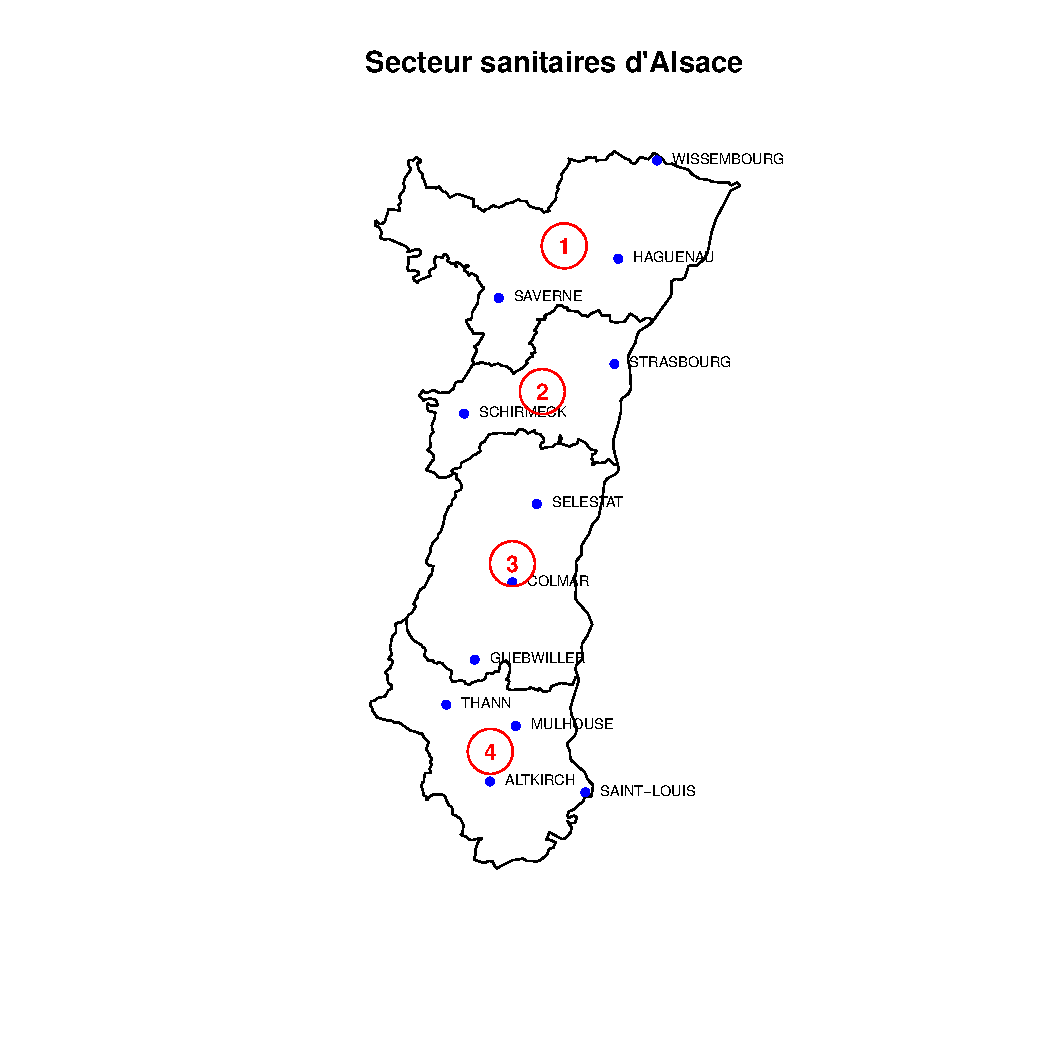
\includegraphics[width=\maxwidth]{figure/carte_secteurs_sanitaires} 

\end{knitrout}



\section{Les territoires de proximité}
\index{Alsace!territoires de proximité}
\index{Territoires de proximité}

Il existe douze territoires de proximité:
\begin{enumerate}
  \item territoire 1: Wissembourg
  \item territoire 2: Haguenau
  \item territoire 3: Saverne
  \item territoire 4: Strasbourg
  \item territoire 5: Molsheim-Schirmeck
  \item territoire 6: Sélestat-Obernai
  \item territoire 7: Colmar
  \item territoire 8: Guebwiller
  \item territoire 9: Thann
  \item territoire 10: Mulhouse
  \item territoire 11: Altkirch
  \item territoire 12: Saint-Louis
\end{enumerate}

% carte des territoires de santé
\begin{figure}[ht]
 \centering
 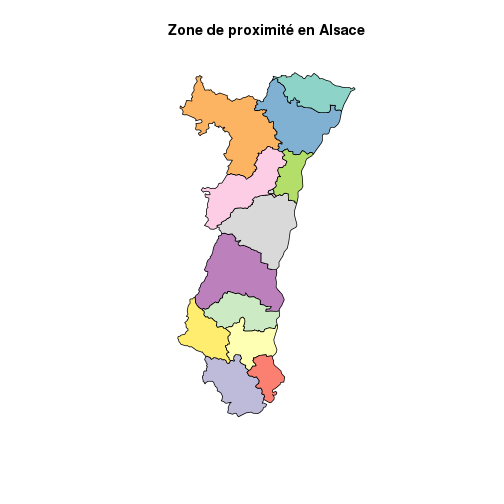
\includegraphics[height=15cm,keepaspectratio=true]{../figure/zone_proximite.png}
 % image.: 0x0 pixel, 0dpi, nanxnan cm, bb=
 \caption{L'Alsace compte 12 territoires de proximité}
 \label{fig:zp}
\end{figure}

\section{Démographie}
\subsection{Généralités}
\index{Alsace!démographie}

En France, les populations légales sont calculées par l'INSEE sur la base de définitions réglementaires à partir de recensement de la population. 
Les populations légales millésimées 2010 entrent en vigueur le 1er janvier 2013.  

\subsubsection{Le concept de population municipale}

Ce document utilise la \emph{Population municipale} \ref{Population_municipale} \index{Population@Population!municipale}  qui est la nouvelle dénomination de la population sans double comptes et qui correspond à la notion de \emph{population} utilisée usuellement en statistique.
Le chiffre est donc inférieur de celui de la \emph{Population totale} qui est égale à la somme de la population municipale et de la population comptée à part d'une commune.
Les chiffres de l'INSEE sont les suivants \footnote{http://www.insee.fr/fr/ppp/bases-de-donnees/recensement/populations-legales/france-regions.asp?annee=2010}:

\begin{table}
\begin{center}
\begin{tabular}{|c|c|}
\hline 
Région & Population\tabularnewline
\hline 
\hline 
France métropolitaine et DOM & 64 612 939\tabularnewline
\hline 
Dont France métropolitaine & 62 765 235\tabularnewline
\hline 
Alsace & 1 845 687\tabularnewline
\hline 
Bas-Rhin & 1 095 905\tabularnewline
\hline 
Haut-Rhin & 749 782\tabularnewline
\hline 
\end{tabular}
\caption[Populations légales 2010]{Populations légales 2010 des régions de France métropolitaine, Population
municipale (Source : Recensement de la population 2010 - Limites territoriales
au 1er janvier 2012) }
\label{pop2010}
\end{center}
\end{table}

\subsection{Classes d'age}
Depuis la mise en place des serveurs régionaux, on a pris l'habitude de diviser la population en trois catégories selon l'age:
\begin{enumerate}
  \item Les moins de un an
  \item de 1 an à 75 ans
  \item les plus de 75 ans
\end{enumerate}

Les calculs sont effectués à partir du fichier \texttt{BTT\_TD\_POP1B\_2010} de l'INSEE qui recense l'ensemble de la population par commune et par tranches de un an. La version utilisée est celle du 1er janvier 2010 (tab.\ref{pop}). Le secteur de proximité de Strasbourg qui est aussi le plus peuplé, compte le plus grand nombre de personnes de 75 ans et plus (figure \ref{fig:75ans} page \pageref{fig:75ans})




\begin{table}
\begin{center}
\begin{tabular}{|l|l|r|r|}
  \hline
  Tranche d'age & Abréviation & Effectif & Pourcentage \\
  \hline
  \hline
   Moins de 1 an & pop0 & \np{21655} & 1.17 \\
   De 1 à 75 ans & pop1\_75 & \np{1677958} & 90.91 \\
   Plus de 75 ans& pop75 & \np{146074} & 7.91 \\
   \hline
   Total & pop\_tot & \np{1845687} & 100.00 \\
  \hline
\end{tabular}
\caption{Classe d'age en Alsace (janvier 2010)}
\label{pop}
\end{center}
\end{table}

% carte des plus de 75 ans
\begin{figure}[ht]
 \centering
 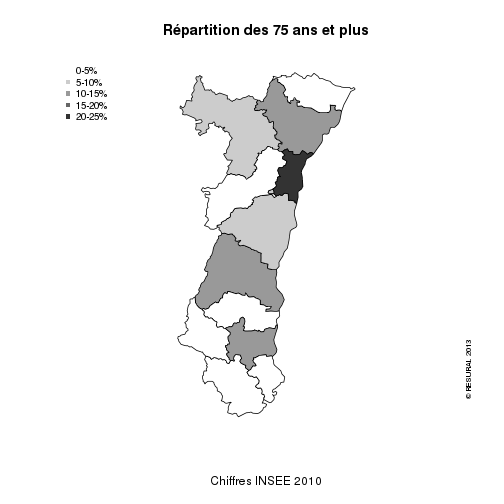
\includegraphics[height=15cm,keepaspectratio=true]{../figure/75ans.png}
 % image.: 0x0 pixel, 0dpi, nanxnan cm, bb=
 \caption[Répartition des 75 ans et plus]{Les personnes de 75 ans et plus en Alsace en fonction du territoire de proximté (en pourcentage du nombre total de 75 ans et plus).}
 \label{fig:75ans}
\end{figure}

\section{Les services d'accueil des urgences (SAU)}
\index{Services d'urgence!en Alsace}
\index{Alsace!services d'urgence}

L'autorisation de pratiquer la médecine d'urgence est délivrée par l'ARS en cohérence avec le schéma régional de l'organisation des soins (SROS) dont les dispositions pour la période 2012-2016 ont été précisées par l'arrêté du 30 janvier 2012 \cite{14} et du 23 mai 2013 \cite{15}.

Rélementairement, le CSP reconnait deux types de structures pouvant être autorisées à prendre en charge directement des patients pouvant relever d'une situation d'urgence
\begin{enumerate}
  \item les structures d'urgence (SU). Le CSP reconnait quatre types d'autorisations qui peuvent être dissociées:
    \begin{itemize}
      \item SAMU
      \item SMUR
      \item SU
      \item SU pédiatrique
    \end{itemize}

  \item les plateaux techniques spécialisés d'accès direct (PTSAD: article R 6123-32-6 CSP) qui sont de quatres types en Alsace:
    \begin{itemize}
      \item Urgences main
      \item Urgences cardiologiques
      \item Urgences neuro vasculaires
      \item Poly-traumatisés
    \end{itemize}
\end{enumerate}

On peut trouver des PTSAD avec une autorisation SU mais qui ne concerne que la spécialité du plateau technique, des PTSAD non labellisé SU, des SU non labellisés pédiatriques mais ayant une activité pédiatrique exclusive.

A la date du 23 mai 2013, l'Alsace compte 18 établissements ou structures autorisés pour l'activité de soins de médecine d'urgence (article R6123-1 du CSP) dont deux ayant une activité de PTDAD exclusive \cite{15}, 1 établissement labellisé SU pédiatrique.

En pratique, à la question qui prend en charge 24h sur 24 des problèmes aigus de santé et/ou de permanence des soins, on se ramène a une listede 14 établissements pratiquant la médecine d'urgence au sens où on l'entend communément. Trois établissements ont une activité multisite. Au final cela représente 18 sites Les trois villes les plus importantes de la région concentrent la totalité des PTSAD.

Celle-ci se pratique au sein de ce qu'il est communément appelé services d'urgence (SU). Le SROS 2 avait introduit une distinction entre les services accueillant les urgences en fonction de leurs capacités et plateau technique. On distinguait alors les UPATOU, les POSU et les SAU. Cette nomenclature qui reposait sur une réalité avait été bien assimilée par les professionnels de santé et beaucoup continuent de l'utiliser,même si elle n'a plus cours officiellement. 

La clinique du Diaconat de Strasbourg,bien que disposant de cette autorisation, ne prend en charge que les urgences mains pour lequelles elle dispose d'une labellisation FESUM \footnote{Federation Européenne des Services d'Urgence de la Main}

On prend également en compte la clinique Saint-Luc de Schirmeck qui fait fonctionner une policlinique recevant plus de \np{8000} passages par an. Officiellement, cet établissement de santé ne dispose pas de cette autorisation bien qu'elle en effectue la mission et est le seul établissement de proximité de la zone Molsheim-Schirmeck.

Les HUS sont le seul établissement d'Alsace a posséder un SU pédiatrique labellisé. Les HUS ont également un service labellisé urgences main (FESUM) situé au CCOM d'Illkirch mais ce dernier n'est pas inclu dans les implantations de services d'urgence.

Sont officiellement labellisés 18 sites (en y incluant SOS main Diaconnat mais pas la clinique St Luc). Ces données sont résumées dans le tableau \ref{tab:sualsace} page \pageref{tab:sualsace}

\begin{landscape}
\begin{table}
\begin{center}
\begin{tabular}{|c|c|c|c|c|c|c|c|c|c|}
\hline 
Territoire & ZProximité & Etablissement & FINESS J & Site & FINESS G & SU & SU Ped & SMUR & SAMU\tabularnewline
\hline 
\hline 
 \multirow{3}{*}{1} & Wissembourg & CH Wissembourg &  & id &  & oui &  & oui & \tabularnewline
\cline{2-10} 
 & Haguenau & CH Haguenau &  & id &  & oui &  & oui & \tabularnewline
\cline{2-10} 
 & Saverne & CH Saverne &  & id &  & oui &  & oui & \tabularnewline
\hline 
\multirow{7}{*}{2} & \multirow{6}{*}{Strasbourg} & \multirow{3}{*}{HUS} &  & NHC &  & oui &  &  & \tabularnewline
\cline{4-10} 
 &  &  &  & HTP &  & oui & oui & oui%
\footnote{SMUR Néonatal%
} & \tabularnewline
\cline{4-10} 
 &  &  &  & PL &  &  &  & oui & oui\tabularnewline
\cline{3-10} 
 &  & Ste Anne &  & id &  & oui &  &  & \tabularnewline
\cline{3-10} 
 &  & Ste Odile &  & id &  & oui &  &  & \tabularnewline
\cline{3-10} 
 &  & Diaconnat &  & id &  & oui%
\footnote{SOS Mains%
} &  &  & \tabularnewline
\cline{2-10} 
 & Schirmeck & St Luc &  & id &  &  &  &  & \tabularnewline
\hline 
\multirow{4}{*}{3} & Sélestat & CH Sélestat &  & id &  & oui &  & oui & \tabularnewline
\cline{2-10} 
 & \multirow{2}{*}{Colmar} & \multirow{2}{*}{CH Colmar} &  & HC &  & oui &  & oui & \tabularnewline
\cline{4-10} 
 &  &  &  & Parc &  &  & oui &  & \tabularnewline
\cline{2-10} 
 & Guebwiller & CH Guebwiller &  & id &  & oui &  &  & \tabularnewline
\hline 
\multirow{5}{*}{4} & \multirow{3}{*}{Mulhouse} & \multirow{2}{*}{CH Mulhouse} &  & EM &  & oui & oui & oui & oui\tabularnewline
\cline{4-10} 
 &  &  &  & St Louis &  & oui &  & oui%
\footnote{antenne SMUR%
} & \tabularnewline
\cline{3-10} 
 &  & Diaconnat-F &  & id &  & oui &  &  & \tabularnewline
\cline{2-10} 
 & Thann & CH Thann &  & id &  & oui &  &  & \tabularnewline
\cline{2-10} 
 & Altkirch & CH Altkirch &  & id &  & oui &  &  & \tabularnewline
\hline
\end{tabular}
 \caption[Structures d'urgence]{Services d'urgence d'Alsace}

\label{tab:sualsace}
\end{center}
\end{table}
\end{landscape}

\begin{figure}[ht]
 \centering
\begin{knitrout}
\definecolor{shadecolor}{rgb}{0.969, 0.969, 0.969}\color{fgcolor}\begin{kframe}


{\ttfamily\noindent\color{warningcolor}{\#\# Warning: impossible d'ouvrir le fichier compressé '../als\_ts.Rda', cause probable : 'Aucun fichier ou dossier de ce type'}}

{\ttfamily\noindent\bfseries\color{errorcolor}{\#\# Error: impossible d'ouvrir la connexion}}\end{kframe}
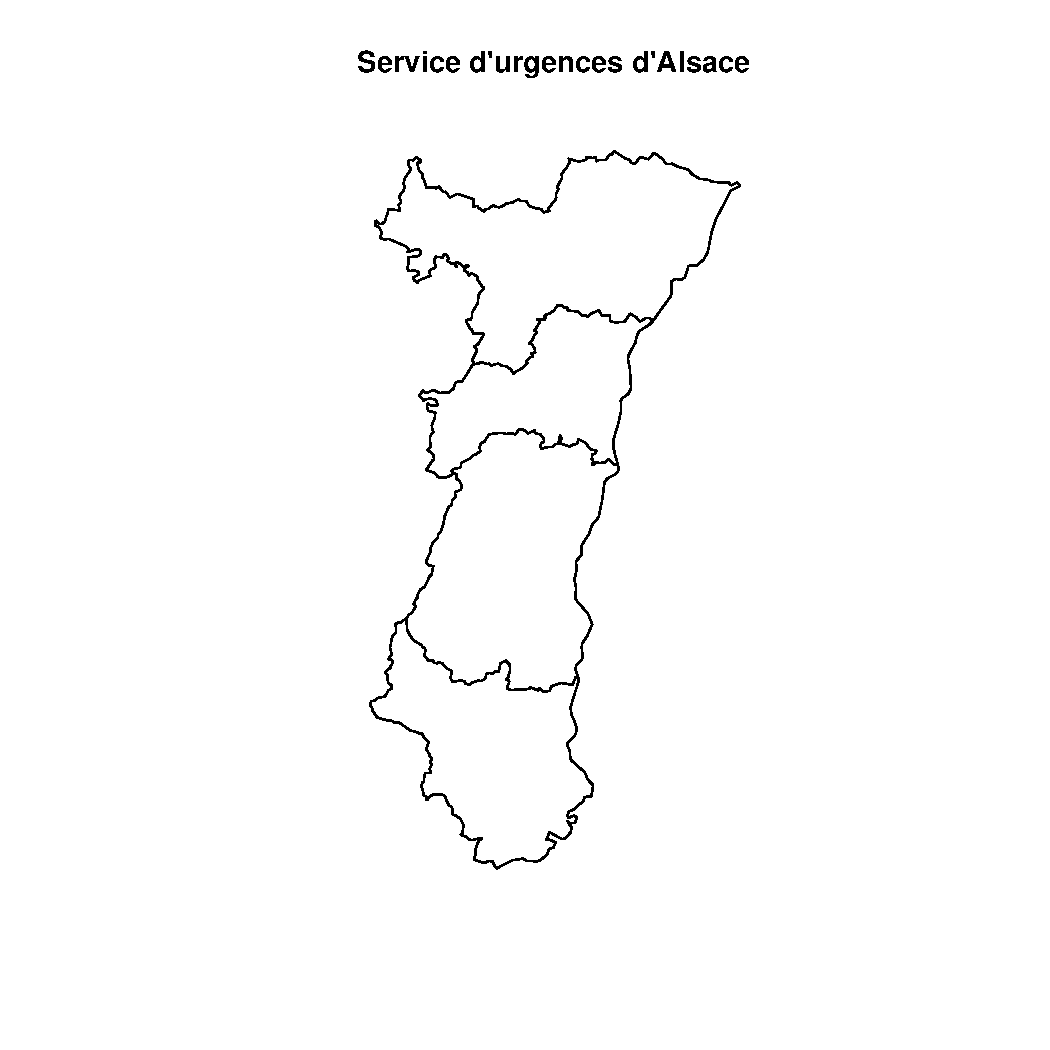
\includegraphics[width=\maxwidth]{figure/carte_sau_2} 
\begin{kframe}

{\ttfamily\noindent\color{warningcolor}{\#\# Warning: impossible d'ouvrir le fichier '../Fichiers source/Hopitaux2lambert/hopitaux\_alsace.csv' : Aucun fichier ou dossier de ce type}}

{\ttfamily\noindent\bfseries\color{errorcolor}{\#\# Error: impossible d'ouvrir la connexion}}

{\ttfamily\noindent\bfseries\color{errorcolor}{\#\# Error: objet 'h' introuvable}}\end{kframe}
\end{knitrout}

 \caption[Services d'urgenced'Alsace]{L'Alsace compte 14 services d'urgence labellisés sur 15 sites.}
 \label{fig:su_alsace}
\end{figure}



\begin{table}
\begin{center}
\begin{tabular}{|c|c|c|c|l|}
  \hline
& Finess utilisé & Finess géographique & Finess Juridique & Structure \\
  \hline
  \hline
1 & 670780055 &   & 670780055 & HUS \\
2 & 670780543 & 670000272 & 670780543 & CH Wissembourg \\
3 & 670000397 & 670000397  & 670780691 & CH Selestat \\
4 & 670780337 & 670000157 & 670780337 & CH Haguenau \\
5 &   & 670000165 & 670780345 & CH Saverne \\
6 & 670016237  & 670016237  & 670016211 & Clinique ste Odile \\
7 &   & 670780212 & 670014604 & Clinique Ste Anne \\
8 & 680000973 & 680000684 & 680000973 & CH Colmar \\
9 & 680000197  & 680000197  & 680000049 & Clinique des trois frontières \\
10 & 680000486 & 680000544  & 680000395 & CH Altkirch \\
11 & 680000700 & 680000700 & 680001005 & CH Guebwiller \\
12 & 680000627 & 680000627 & 680000486 & CH Mulhouse FG \\
13 &   & 680000601 & 680000437 & CH Thann \\
14 &   & 680000320  & 680000643 & Diaconat-Fonderie (St Sauveur) \\
\hline
\end{tabular}
\caption{Service d'accueil des urgences d'Alsace}
\label{summary}
\end{center}
\end{table}


\newpage
\chapter{Les acteurs}

% acteurs.Rnw

% penser au secteur libéral

\section{Exhaustivité quantitative}



On dédinit l'exhaustivité quantitative comme le nombre de RPU transmis par rapport au nombre de passages réels.
Les données proviennent des RPU produits par les hôpitaux d'Alsace ayant l'autorisation de faire fonctionner un service d'urgence (SU). La liste des structures hospitalières ayant fournit des informations alimentant le présent rapport est fournie par la table \ref{tab1}, page \pageref{tab1}.

Tous ces hôpitaux fournissent des données depuis le premier janvier 2013 sauf le CH Saverne qui a commencé en Juillet 2013.

Deux structures ne fournissent pas encore de RPU. Il s'agit de la clinique Sainte-Anne à Strasbourg (Groupe hospitalier Saint-Vincent) et du Centre Hospitalier de Thann.

Certaines données peuvent être recoupées avec celles du serveur régional mis en place en 2006 par l'ARS: 

\fbox{Voir SAU2013}

% latex table generated in R 3.0.2 by xtable 1.7-1 package
% Sat Dec 21 11:32:13 2013
\begin{table}[ht]
\centering
\begin{tabular}{|l|r|r|l|r|}
  \hline
 & n & \% & Hôpitaux & Date d'inclusion \\ 
  \hline
3Fr & 14431 & 4.78 & Clinique des 3 frontières & 01/01/2013 \\ 
  Alk & 6457 & 2.14 & CH Altkirch & 01/04/2013 \\ 
  Col & 59503 & 19.72 & CH Colmar & 01/01/2013 \\ 
  Dia & 26976 & 8.94 & Diaconat Fonderie & 01/01/2013 \\ 
  Geb & 13900 & 4.61 & CH Guebwiller & 01/01/2013 \\ 
  Hag & 31834 & 10.55 & CH Haguenau & 01/01/2013 \\ 
  Hus & 33907 & 11.24 & Hôpitaux Universitaires de Strasbourg & 01/01/2013 \\ 
  Mul & 50982 & 16.89 & CH Mulhouse & 07/01/2013 \\ 
  Odi & 23747 & 7.87 & Clinique Ste Odile & 01/01/2013 \\ 
  Sel & 18502 & 6.13 & CH Sélestat & 01/01/2013 \\ 
  Wis & 11613 & 3.85 & CH Wissembourg & 01/01/2013 \\ 
  Sav & 9915 & 3.29 & CH Saverne & 23/07/2013 \\ 
   \hline
\end{tabular}
\caption{Structures hospitalières participantes en 2013} 
\label{tab1}
\end{table}



\section{Exhaustivité qualitative}

L'exhaustivité qualitative correspond à la fois à la complétude des items et à la cohérence de réponses.

Les informations de nature administrative (code postal, commune d'origine, sexe, date de naissance,\dots ) sont correctement renseignées avec une exhaustivité de $100\%$.

Les données à caractère plus médical comme le motif de consultation ou le diagnostic principal ont une exhaustivité moins bonne, de l'ordre de $70\%$.

% latex table generated in R 3.0.2 by xtable 1.7-1 package
% Sat Dec 21 11:32:13 2013
\begin{table}[ht]
\centering
\begin{tabular}{|l|r|}
  \hline
 & \% \\ 
  \hline
id & 0.00 \\ 
  CODE\_POSTAL & 0.00 \\ 
  COMMUNE & 0.00 \\ 
  ENTREE & 0.00 \\ 
  EXTRACT & 0.00 \\ 
  FINESS & 0.00 \\ 
  NAISSANCE & 0.00 \\ 
  SEXE & 0.00 \\ 
  AGE & 0.00 \\ 
  secteur & 0.00 \\ 
  SORTIE & 9.15 \\ 
  MODE\_ENTREE & 10.01 \\ 
  GRAVITE & 14.50 \\ 
  MODE\_SORTIE & 14.53 \\ 
  TRANSPORT & 23.43 \\ 
  TRANSPORT\_PEC & 26.05 \\ 
  DP & 34.17 \\ 
  PROVENANCE & 35.81 \\ 
  MOTIF & 36.72 \\ 
  DESTINATION & 78.81 \\ 
  ORIENTATION & 80.04 \\ 
   \hline
\end{tabular}
\caption{Données manquantes en 2013} 
\label{tab2}
\end{table}



Les informations sont résumées dans la table \ref{tab2}, page \pageref{tab2}.

\section{Diagramme de complétude}

On peut représenter sous forme d'un diagramme en radar (ou toile d'araignée) l'exhaustivité qualitative des données. Chaque item du RPU est représenté par le rayon d'une roue, gradué de 0 à 100\%. Sur chaque rayon, les points obtenus sont reliés entre eux pour dessiner un polygone qui figue la physionomie de l'ensemble des données.

\begin{knitrout}
\definecolor{shadecolor}{rgb}{0.969, 0.969, 0.969}\color{fgcolor}\begin{kframe}
\begin{verbatim}
##            id   CODE_POSTAL       COMMUNE   DESTINATION            DP 
##          0.00          0.00          0.00         78.81         34.17 
##        ENTREE       EXTRACT        FINESS       GRAVITE   MODE_ENTREE 
##          0.00          0.00          0.00         14.50         10.01 
##   MODE_SORTIE         MOTIF     NAISSANCE   ORIENTATION    PROVENANCE 
##         14.53         36.72          0.00         80.04         35.81 
##          SEXE        SORTIE     TRANSPORT TRANSPORT_PEC           AGE 
##          0.00          9.15         23.43         26.05          0.00 
##       secteur 
##          0.00
\end{verbatim}


{\ttfamily\noindent\color{warningcolor}{\#\# Warning: 'x' is NULL so the result will be NULL\\\#\# Warning: 'x' is NULL so the result will be NULL}}\end{kframe}
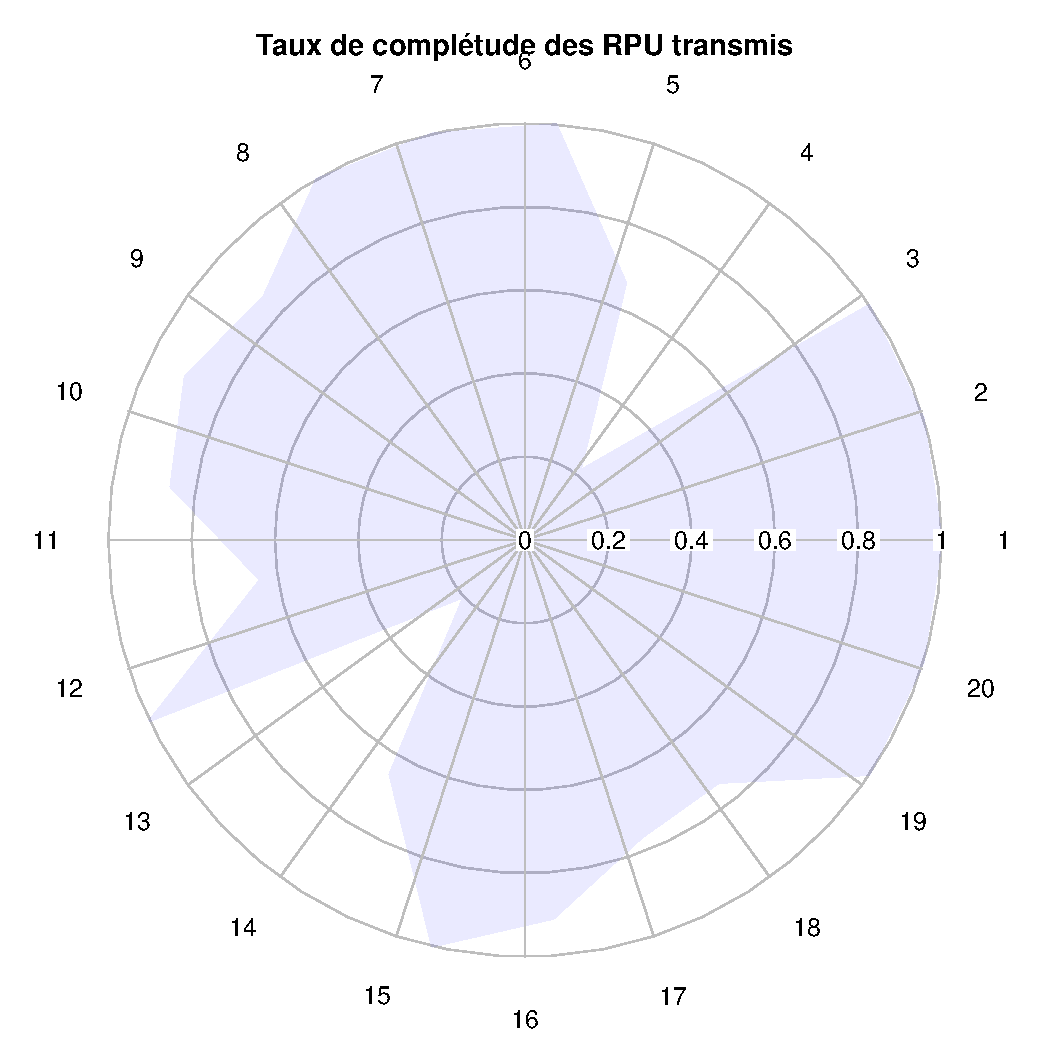
\includegraphics[width=\maxwidth]{figure/radar} 

\end{knitrout}


Le renseignement des items varie entre $20\%$ et $100\%$. Cependant ces données sont à interpréter avec prudence. Ainsi l'item 4 qui correspond au mode de sortie ne distingue pas les non réponses des vrais retours à domicile (se reporter à la discussion page \pageref{ref:sortie})


\newpage
\chapter{RESURAL}

% resural.Rnw
\index{RESURAL}

Le réseau des urgences en Alsace (RESURAL) est une association à but non lucratif, de droit local Alsace-Moselle, dont les statuts sont déposés au tribunal de Strasbourg. Le réseau a été fondé en août 2008. En son membre de droit les services d'urgence intra et extra-hospitaliers, adultes et pédiatriques, possédant une autorisation d'exercer cette spécialité, délivrée par l'agence régionale de santé (ARS). \index{ARS}

Elle est domiciliée aux Hôpitaux Universitaires de Strasbourg.

Elle est dirigée par un conseil d'administration et représentée par son preésident, le Docteur Bruno Goulesque.

Son fonctionnement est assuré par une équipe de coordination, composée d'un médecin coordinateur à mi-temps et d'une assistante à mi-temps. Cette équipe est opérationnelle depuis le 1er février 2013.


\newpage
\chapter{L'observatoire des urgences en Alsace (ORUDAL)}

% orudal.Rnw

L'observatoire des urgences en Alsace (ORUDAL) est une structure informelle animée par le réseau des urgences en Alsace.
\index{ORUDAL}
\index{Observatoire des urgences en Alsace}

Il est composé des organismes suivants:
\begin{enumerate}
  \item RESURAL \index{RESURAL}
  \item ARS Alsace
  \item CIRE-InVS
  \item Alsace e-santé
  \item CMUNE
\end{enumerate}


\section*{Les partenaires}

  \subsection*{Agence Régionale de Santé}
    \index{ARS}
    
  \subsection*{Alsace e-santé}
    \index{Alsace e-santé}
    
  \subsection*{CIRE-INVS}
    \index{CIRE-INVS}
    
  \subsection*{Collège de médecine d'urgence (CMUNE)}
    \index{CMUNE}

\section*{FEDORU}
  \index{FEDORU}
  
La fédération des observatoires des urgences et structures apparentés a été crée en octobre 2013 à l'initiative de quelques organisme régionaux dont Résural sur une proposition de l'ORUPACA \index{ORUPACA}


\newpage
\chapter{Le Résumé du passage aux urgences}

% rpu.Rnw

\index{RPU}
\index{Résumé du passage aux urgences}

La création du résumé des passages aux urgences (RPU) remonte à 2002 \cite{11}. Sur la base d'un projet pilote mené par l'ORUMIP, la DHOS, à l'initiative de son directeur Edouard Couty, lance sur la base du volontariat, la collecte des RPU.

\section*{RPU}

% Les Résumés de Passage aux Urgences (RPU) ont été transmis par le Centre Hospitalier de Sélestat à partir de 2008. 
% La table \emph{rpu} du serveur de test comporte nrow(d2) lignes et ncol(d2) colonnes. La période érudiée couvre toute l'année 2009 s'étend (du d2$date_entree[1] au d2$date_entree[nrow(d2)]), ce qui correspond à toutes les entrées de cette année. Les RPU sont saisis selon la version 5 du cahier des charges transmis par l'INVS (version du 31 janvier 2007).
% \\
Chaque passage aux urgences donne lieu à la création d'un RPU qui collecte les informations suivantes:
\begin{enumerate}
  \item l'établissement de santé, siège du SAU (FINESS géographique)
  \item code postal de résidence
  \item commune de résidence
  \item date de naissance
  \item sexe
  \item date et heure d'entrée
  \item mode d'entrée
  \item provenance du patient
  \item mode de transport
  \item mode de prise en charge
  \item le motif de recours aux urgences
  \item la gravité
  \item le diagnostic principal
  \item le(s) diagnostic(s) associé(s)
  \item les actes médicaux
  \item le mode de sortie
  \item l'orientation du patient
  \item date et heure de sortie
\end{enumerate}

%%%%%%%%%%%%%%
\subsubsection{L'identifiant (ID)}
%%%%%%%%%%%%%%

Ils'agit d'un code unique caractérisant le RPU. Il ne fait pas partie de la définition de l'INVS.Il a été rajouté par SAGEC à l'origine du serveur régional pour retrouver l'enregistrement en cas de problème et faciliter laliaison avec d'autres rubriques comme les diagnostiques associés.

%%%%%%%%%%%%%%
\subsubsection{L'établissement de santé}
%%%%%%%%%%%%%%

\index{FINESS}
Il est identifié par son numéro FINESS. Le schéma de l'INVS ne précise pas quel FINESS utiliser et on trouve des FINESS juridiques et géographiques. Nous recommandons d'utiliser le FINESS géographique qi permet d'identifier la structure d'origine quand il s'agit d'établissements multisites.

%%%%%%%%%%%%%%
\subsubsection{Le code postal de résidence}
%%%%%%%%%%%%%%

\index{code postal}
Lorsque le lieu de résidence se situe hors des limites du territoire national, il faut indiquer par convention $99999$.
Si le code postal précis est inconnu : le numéro du département suivi de 999
Pour les malades résidant hors de France : 99 suivi du code INSEE du pays \footnote{http://www.insee.fr/fr/methodes/nomenclatures/cog/pays.asp}
Si le département ou le pays de résidence est inconnu : 99999

%%%%%%%%%%%%%%
\subsubsection{le motif de recours aux urgences}
%%%%%%%%%%%%%%

\index{motif de recours}
Il faut utiliser l'un des motifs de recours préconisé par le ministère de la santé \cite{13} et codifiés par la SFMU. La dernière version est la version de juin 2013 du thésaurus de la SFMU accessible sur le site internet de cette dernière. Il comporte une liste d'environ $150$ recours avec leur équivalence CIM10.

%%%%%%%%%%%%%%
\subsubsection{Le mode de sortie}
%%%%%%%%%%%%%%

\index{mode de sortie}
\index{retour à domicile}
\label{ref:sortie}
Les patients quittent les urgences soit parcequ'ils ne nécessitent pas d'hospitalisation (c'est un \emph{retour à domicile}), soit parcequ'ils sont hospitalisé dans la structure hospitalière (c'est une \emph{mutation}\index{mutation}) ou dans un autre établissement (on parle alors de \emph{transfert}\index{transfert}). Enfin il peut s'agir d'un \emph{décès}\index{décès} dans le service d'urgence.

\begin{itemize}
  \item « 6 » Mutation : le malade est hospitalisé vers une autre unité médicale de la même
entité juridique \footnote{Dans les établissements privés visés aux alinéas d et e de l'article L162-22-6 du code de la sécurité sociale (CSS), si le patient provient d’un autre établissement de la même entité juridique, le mode desortie à utiliser est le 7}
  \item « 7 » Transfert : le malade est hospitalisé dans une autre entité juridique
  \item « 8 » Domicile : le malade retourne au domicile ou son substitut, tel une
structure d'hébergement médico-social.
  \item « 9 » Décès : le malade décède aux urgences
\end{itemize}

Cette rubrique est détaillée par les items \emph{destination} et \emph{orientation}

%%%%%%%%%%%%%%
\subsubsection{Destination}
%%%%%%%%%%%%%%

En cas de sortie par mutation ou transfert, il peut s'agir:
\begin{itemize}
  \item « 1 » Hospitalisation dans une unité de soins de courte durée (MCO)\index{MCO}
  \item « 2 » Hospitalisation dans une unité de soins de suite ou de réadaptation (SSR)\index{SSR}
  \item « 3 » Hospitalisation dans une unité de soins de longue durée (SLD)\index{SLD}
  \item « 4 » Hospitalisation dans une unité de psychiatrie (PSY)\index{PSY}
\end{itemize}

En cas de sortie au domicile
\begin{itemize}
  \item « 6 » Retour au domicile dans le cadre d’une hospitalisation à domicile (HAD)\index{HAD}
  \item « 7 » Retour vers une structure d'hébergement médico-social (HMS)\index{HMS}
\end{itemize}

On notera que dans cette formulation, le retour à domicile "normal" est implicite et celà génère une ambiguité car si la rubrique est laissée libre, on ne saitpas s'il s'agit d'une non réponse ou d'un retour simple à domicile.

%%%%%%%%%%%%%%
\subsubsection{Orientation}
%%%%%%%%%%%%%%

\index{orientation}
L'orientation précise le devenir ou les circonstances associées. Cette rubrique est complémentaire du \emph{mode de sortie}. Malheureusement, elle souffre de la mêmelimitation:le retour à domicile simple est implicite.

\begin{enumerate}
  \item En cas de sortie par mutation ou transfert
    \begin{itemize}
      \item « HDT » hospitalisation sur la demande d’un tiers
      \item « HO » hospitalisation d’office
      \item « SC » hospitalisation dans une unité de Surveillance Continue
      \item « SI » hospitalisation dans une unité de Soins Intensifs
      \item « REA » hospitalisation dans une unité de Réanimation
      \item « UHCD » hospitalisation dans une unité d’hospitalisation de courte durée
      \item « MED » hospitalisation dans une unité de Médecine hors SC, SI, REA
      \item « CHIR» hospitalisation dans une unité de Chirurgie hors SC, SI, REA
      \item « OBST» hospitalisation dans une unité d’Obstétrique hors SC, SI, REA
    \end{itemize}

  \item En cas de sortie au domicile
    \begin{itemize}
      \item « FUGUE » sortie du service à l’insu du personnel soignant
      \item « SCAM » sortie contre avis médical
      \item « PSA » partie sans attendre prise en charge
      \item « REO » réorientation directe sans soins (ex vers consultation spécialisée ou   lorsque le service d’accueil administratif est fermée)
    \end{itemize}

\end{enumerate}





%========================================================== PARTIE 2
\part{Activité des services d'urgence d'Alsace}

\newpage
\chapter{Activité régionale totale}
\section{Nombre total de passages}

% activite_regionale.Rnw

%on fabrique un objet **a** qui fait la somme par date des passages aux urgences:



% vérification:
%   a[1:10]
% 2013-01-01 2013-01-02 2013-01-03 2013-01-04 2013-01-05 2013-01-06 2013-01-07 2013-01-08 2013-01-09 2013-01-10 
%        884        801        686        704        722        691        876        694        683        673 
% On supprime l'enregistrement 211 correspondant au 31 juillet et qui ne contient que 2 éléments:
%a[211]  2013-07-31 2 


% Min. 1 st Qu.  Median    Mean 3rd Qu.    Max. 
%   642.0   848.0   895.5   883.2   957.0  1050.0 

L'ensemble des SU ont déclaré \np{301767} passages au 30 novembre 2013, 
soit une moyenne de \np{906} passages par jour (extrèmes 642 et \np{1160})

Passages par secteur sanitaire:


\begin{table}[ht]
\centering
\begin{tabular}{rr}
  \hline
 Territoire & RPU déclarés \\ 
  \hline
  1 & \np{53362} \\ 
  2 & \np{57654} \\ 
  3 & \np{91905} \\ 
  4 & \np{98846} \\ 
   \hline
\end{tabular}
\end{table}

Les données du secteur 2 sont très sous-estimées car il manque celles de la Clinique Sainte-Anne, des urgences pédiatriques de Hautepierre ainsi q'une part importante des RPU des urgences adulte des HUS.


%affichage du graphique
\begin{knitrout}
\definecolor{shadecolor}{rgb}{0.969, 0.969, 0.969}\color{fgcolor}
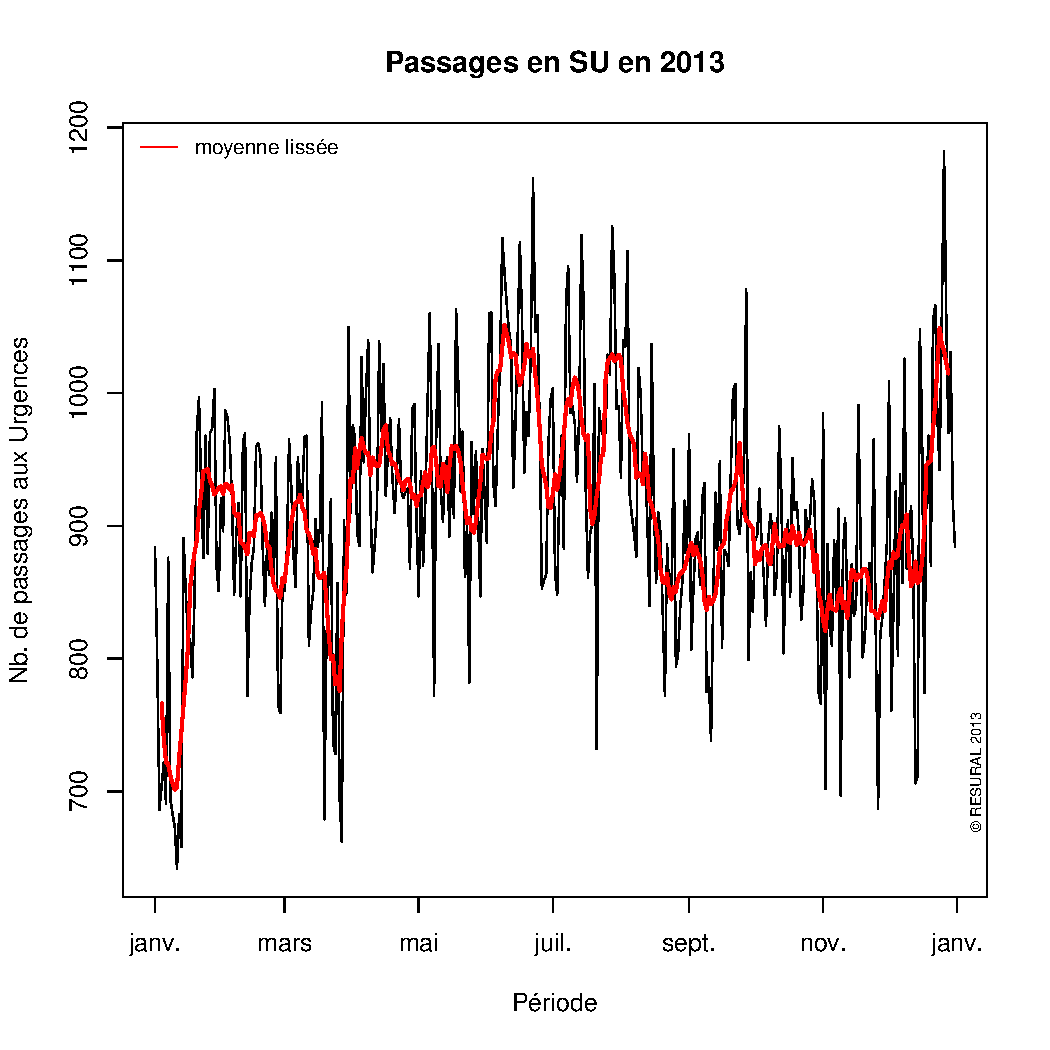
\includegraphics[width=\maxwidth]{figure/activite_plot} 

\end{knitrout}

% Variante avec *xts*
\begin{knitrout}
\definecolor{shadecolor}{rgb}{0.969, 0.969, 0.969}\color{fgcolor}
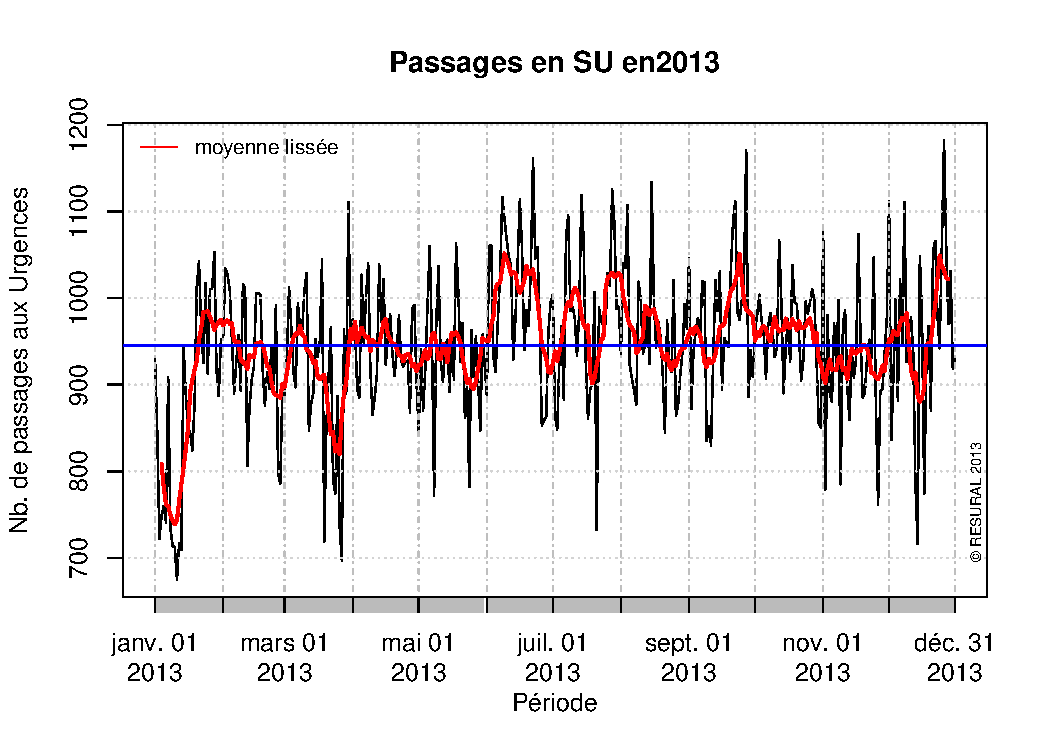
\includegraphics[width=\maxwidth]{figure/activite_plot2} 

\end{knitrout}


\subsection*{En valeur absolue}
% latex table generated in R 3.0.2 by xtable 1.7-1 package
% Sat Dec 21 11:32:18 2013
\begin{table}[ht]
\centering
\begin{tabular}{llr}
  \hline
 & Hôpital & RPU \\ 
  \hline
1 & 3Fr & 14431 \\ 
  2 & Alk & 6457 \\ 
  3 & Col & 59503 \\ 
  4 & Dia & 26976 \\ 
  5 & Geb & 13900 \\ 
  6 & Hag & 31834 \\ 
  7 & Hus & 33907 \\ 
  8 & Mul & 50982 \\ 
  9 & Odi & 23747 \\ 
  10 & Sel & 18502 \\ 
  11 & Wis & 11613 \\ 
  12 & Sav & 9915 \\ 
   \hline
\end{tabular}
\caption[Nombre de passages par service d'urgence]{Passages par service d'urgence} 
\label{fig:passage_su}
\end{table}

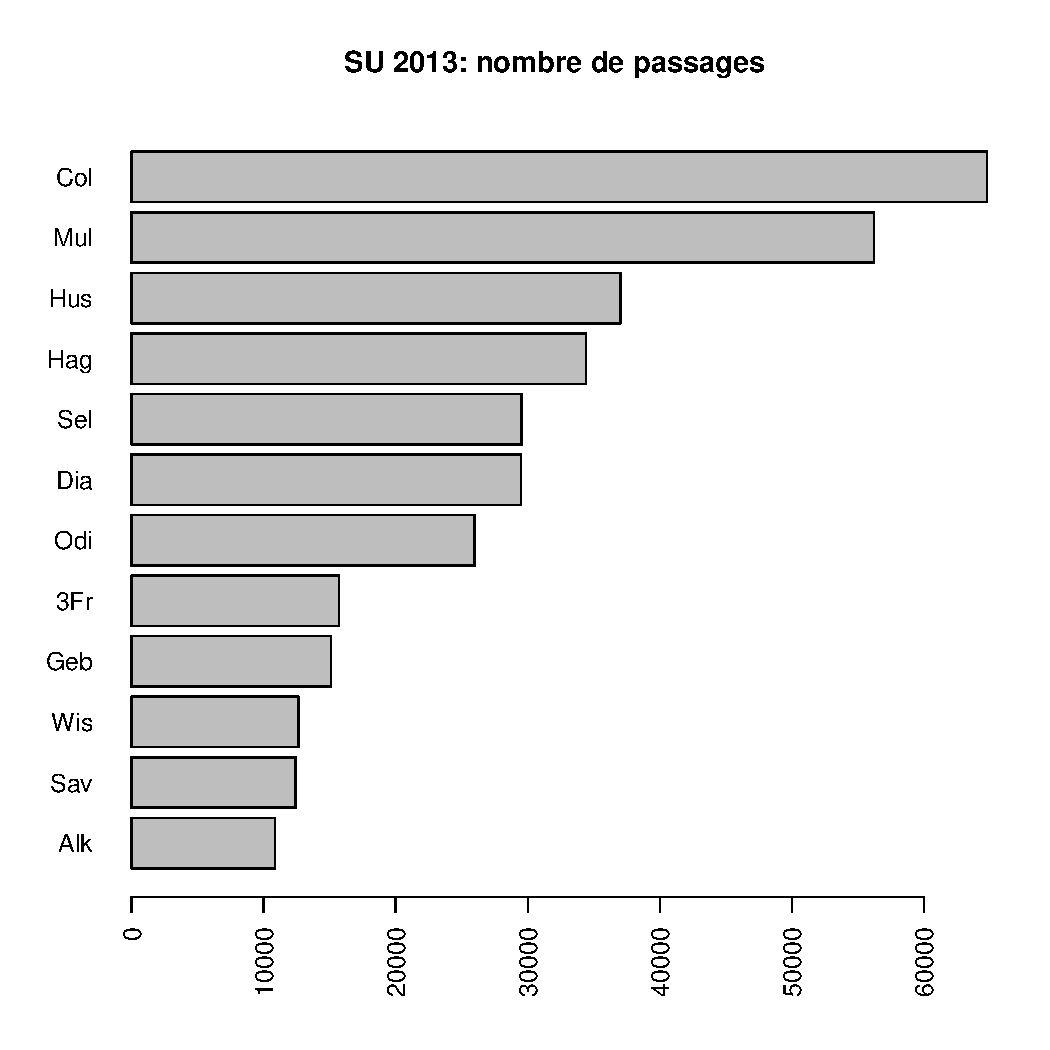
\includegraphics[width=\maxwidth]{figure/val_abs} 



\subsection*{En pourcentage}
\begin{knitrout}
\definecolor{shadecolor}{rgb}{0.969, 0.969, 0.969}\color{fgcolor}
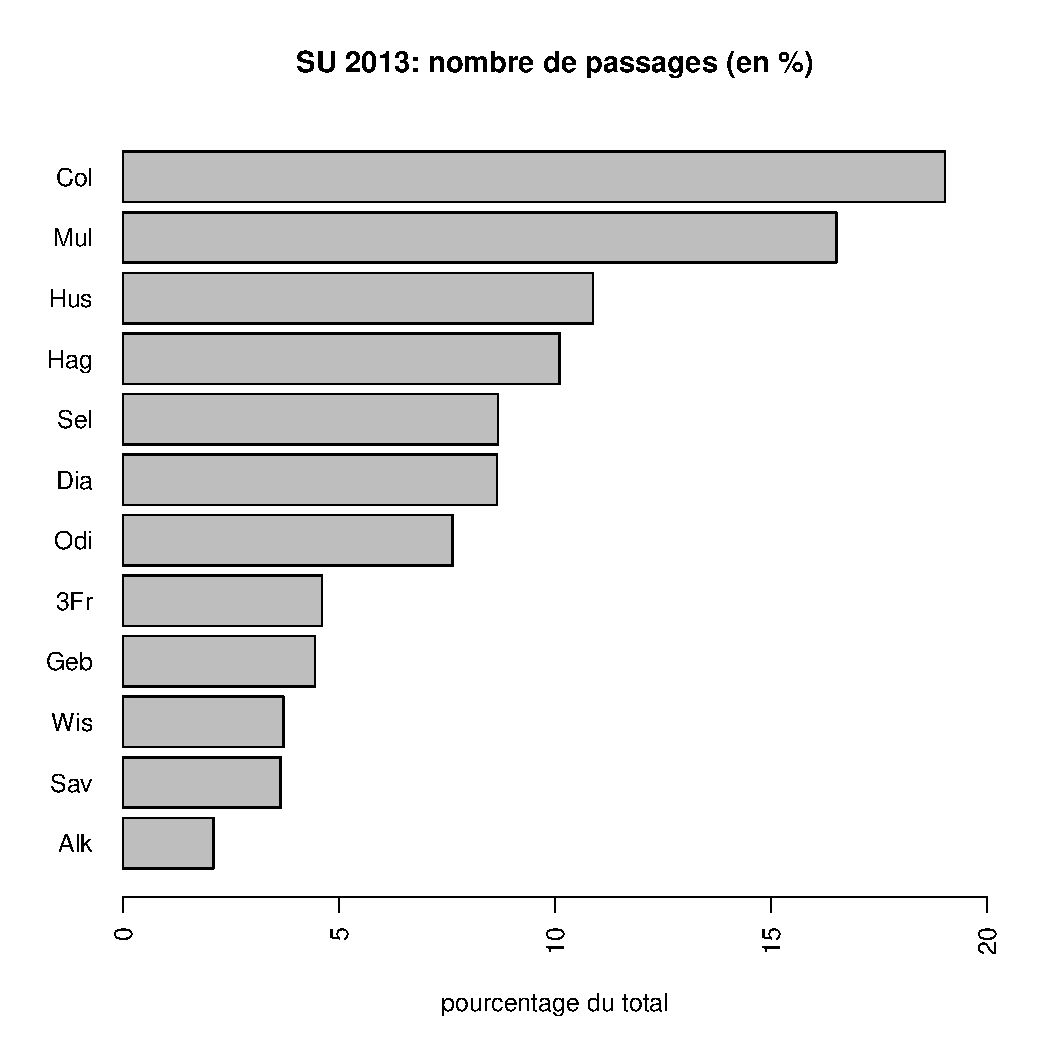
\includegraphics[width=\maxwidth]{figure/en_pourcentage} 

\end{knitrout}


\subsection*{Taux de recours aux urgences}
\begin{knitrout}
\definecolor{shadecolor}{rgb}{0.969, 0.969, 0.969}\color{fgcolor}\begin{kframe}
\begin{verbatim}
## [1] 441062
\end{verbatim}
\end{kframe}
\end{knitrout}

Le taux de recours aux urgences \index{taux de recours aux urgences} (TRU) \index{TRU} est défini comme le nombre total de passages aux urgences, rapporté à la population de la région (INSEE 1er janvier 2010). En Lorraine, ce taux est estimé à 23,45\% en 2010 (\cite{2,3}). En supposant que la population alsacienne se comprte comme la population lorraine, le nombre de passages aux urgences devrait s'établir à \ensuremath{4.4106\times 10^{5}}.

Le TRU 2013 estimé en Alsace à partir des RPU transmis est de 16.04\%.

\subsection*{Activité par mois}
%------------------------------
\begin{knitrout}
\definecolor{shadecolor}{rgb}{0.969, 0.969, 0.969}\color{fgcolor}\begin{kframe}
\begin{alltt}
\hlstd{m} \hlkwb{<-} \hlkwd{month}\hlstd{(d1}\hlopt{$}\hlstd{ENTREE,} \hlkwc{label} \hlstd{=} \hlnum{TRUE}\hlstd{)}
\hlkwd{table}\hlstd{(m)}
\end{alltt}
\begin{verbatim}
## m
##   Jan   Feb   Mar   Apr   May   Jun   Jul   Aug   Sep   Oct   Nov   Dec 
## 25609 25004 26937 28428 27899 30038 30103 28333 26688 27413 25315     0
\end{verbatim}
\begin{alltt}
\hlkwd{barplot}\hlstd{(}\hlkwd{table}\hlstd{(m),} \hlkwc{ylab} \hlstd{=} \hlstr{"nombre"}\hlstd{,} \hlkwc{xlab} \hlstd{=} \hlstr{"mois"}\hlstd{,} \hlkwc{main} \hlstd{=} \hlstr{"2013 - Nombre de RPU par mois"}\hlstd{,}
    \hlkwc{names.arg} \hlstd{=} \hlkwd{c}\hlstd{(}\hlstr{"Jan"}\hlstd{,} \hlstr{"Fev"}\hlstd{,} \hlstr{"Mar"}\hlstd{,} \hlstr{"Avr"}\hlstd{,} \hlstr{"Mai"}\hlstd{,} \hlstr{"Jui"}\hlstd{,} \hlstr{"Jul"}\hlstd{,} \hlstr{"Aou"}\hlstd{,} \hlstr{"Sep"}\hlstd{,}
        \hlstr{"Oct"}\hlstd{,} \hlstr{"Nov"}\hlstd{,} \hlstr{"Dec"}\hlstd{),} \hlkwc{las} \hlstd{=} \hlnum{2}\hlstd{)}
\end{alltt}
\end{kframe}
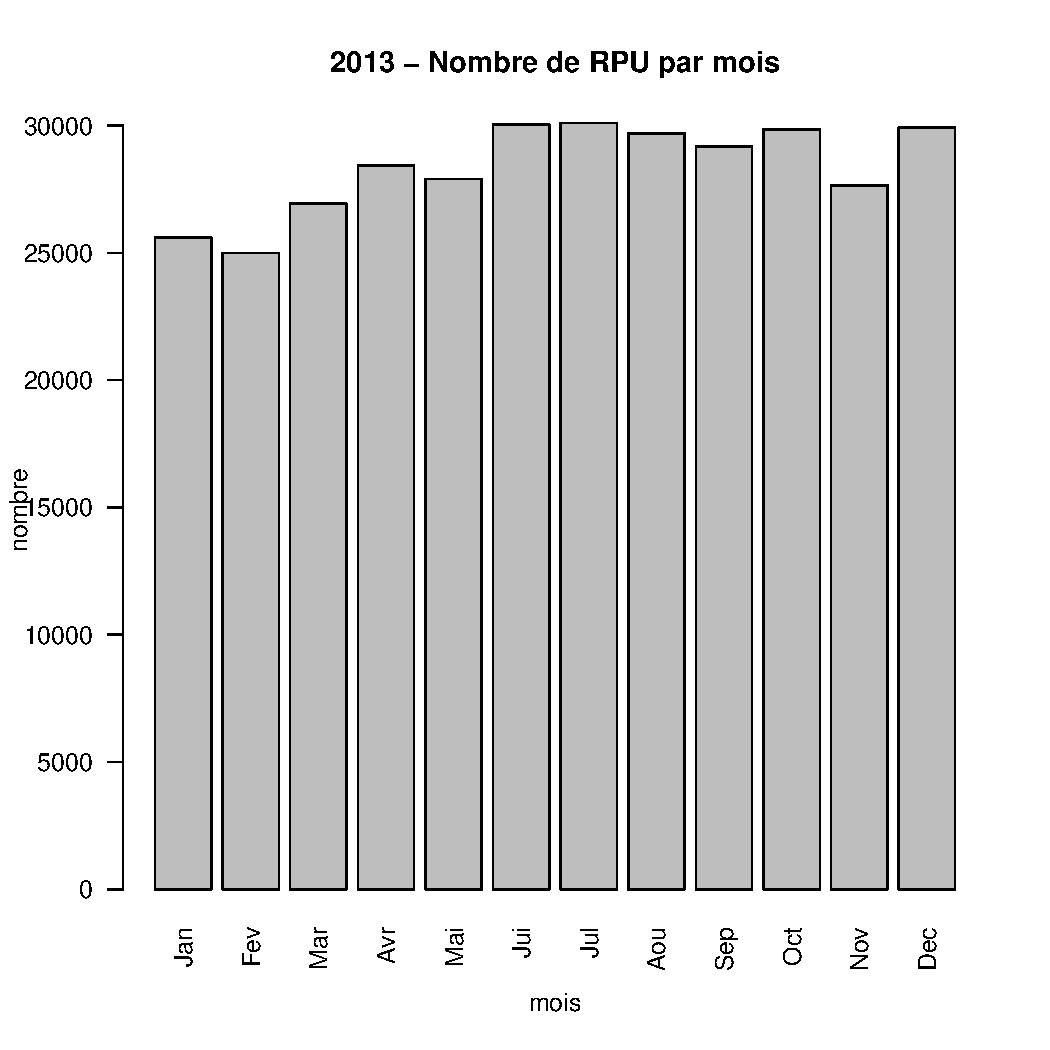
\includegraphics[width=\maxwidth]{figure/parmois} 

\end{knitrout}


\subsection*{Activité par semaine}

% latex table generated in R 3.0.2 by xtable 1.7-1 package
% Sat Dec 21 11:32:20 2013
\begin{table}[ht]
\centering
\begin{tabular}{rr}
  \hline
 & m \\ 
  \hline
1 & 4488 \\ 
  2 & 4909 \\ 
  3 & 5975 \\ 
  4 & 6593 \\ 
  5 & 6509 \\ 
  6 & 6354 \\ 
  7 & 6262 \\ 
  8 & 6193 \\ 
  9 & 6028 \\ 
  10 & 6426 \\ 
  11 & 6152 \\ 
  12 & 5735 \\ 
  13 & 5926 \\ 
  14 & 6698 \\ 
  15 & 6632 \\ 
  16 & 6667 \\ 
  17 & 6538 \\ 
  18 & 6462 \\ 
  19 & 6628 \\ 
  20 & 6720 \\ 
  21 & 6314 \\ 
  22 & 5615 \\ 
  23 & 7116 \\ 
  24 & 7213 \\ 
  25 & 7193 \\ 
  26 & 6569 \\ 
  27 & 6566 \\ 
  28 & 7083 \\ 
  29 & 6391 \\ 
  30 & 7069 \\ 
  31 & 6995 \\ 
  32 & 6726 \\ 
  33 & 6436 \\ 
  34 & 5998 \\ 
  35 & 6049 \\ 
  36 & 6191 \\ 
  37 & 5888 \\ 
  38 & 6331 \\ 
  39 & 6536 \\ 
  40 & 6160 \\ 
  41 & 6210 \\ 
  42 & 6217 \\ 
  43 & 6200 \\ 
  44 & 5944 \\ 
  45 & 5860 \\ 
  46 & 5957 \\ 
  47 & 6074 \\ 
  48 & 4971 \\ 
   \hline
\end{tabular}
\caption[Activité par semaine]{Activité des SU par semaine en 2013} 
\label{act_sem}
\end{table}
% latex table generated in R 3.0.2 by xtable 1.7-1 package
% Sat Dec 21 11:32:20 2013
\begin{table}[ht]
\centering
\begin{tabular}{rrrrrrrrrrrrrrrrrrrrrrrrrrrrrrrrrrrrrrrrrrrrrrrrr}
  \hline
 & 1 & 2 & 3 & 4 & 5 & 6 & 7 & 8 & 9 & 10 & 11 & 12 & 13 & 14 & 15 & 16 & 17 & 18 & 19 & 20 & 21 & 22 & 23 & 24 & 25 & 26 & 27 & 28 & 29 & 30 & 31 & 32 & 33 & 34 & 35 & 36 & 37 & 38 & 39 & 40 & 41 & 42 & 43 & 44 & 45 & 46 & 47 & 48 \\ 
  \hline
1 & 4488 & 4909 & 5975 & 6593 & 6509 & 6354 & 6262 & 6193 & 6028 & 6426 & 6152 & 5735 & 5926 & 6698 & 6632 & 6667 & 6538 & 6462 & 6628 & 6720 & 6314 & 5615 & 7116 & 7213 & 7193 & 6569 & 6566 & 7083 & 6391 & 7069 & 6995 & 6726 & 6436 & 5998 & 6049 & 6191 & 5888 & 6331 & 6536 & 6160 & 6210 & 6217 & 6200 & 5944 & 5860 & 5957 & 6074 & 4971 \\ 
   \hline
\end{tabular}
\caption[Activité par semaine]{Activité des SU par semaine en 2013} 
\label{act_sem2}
\end{table}

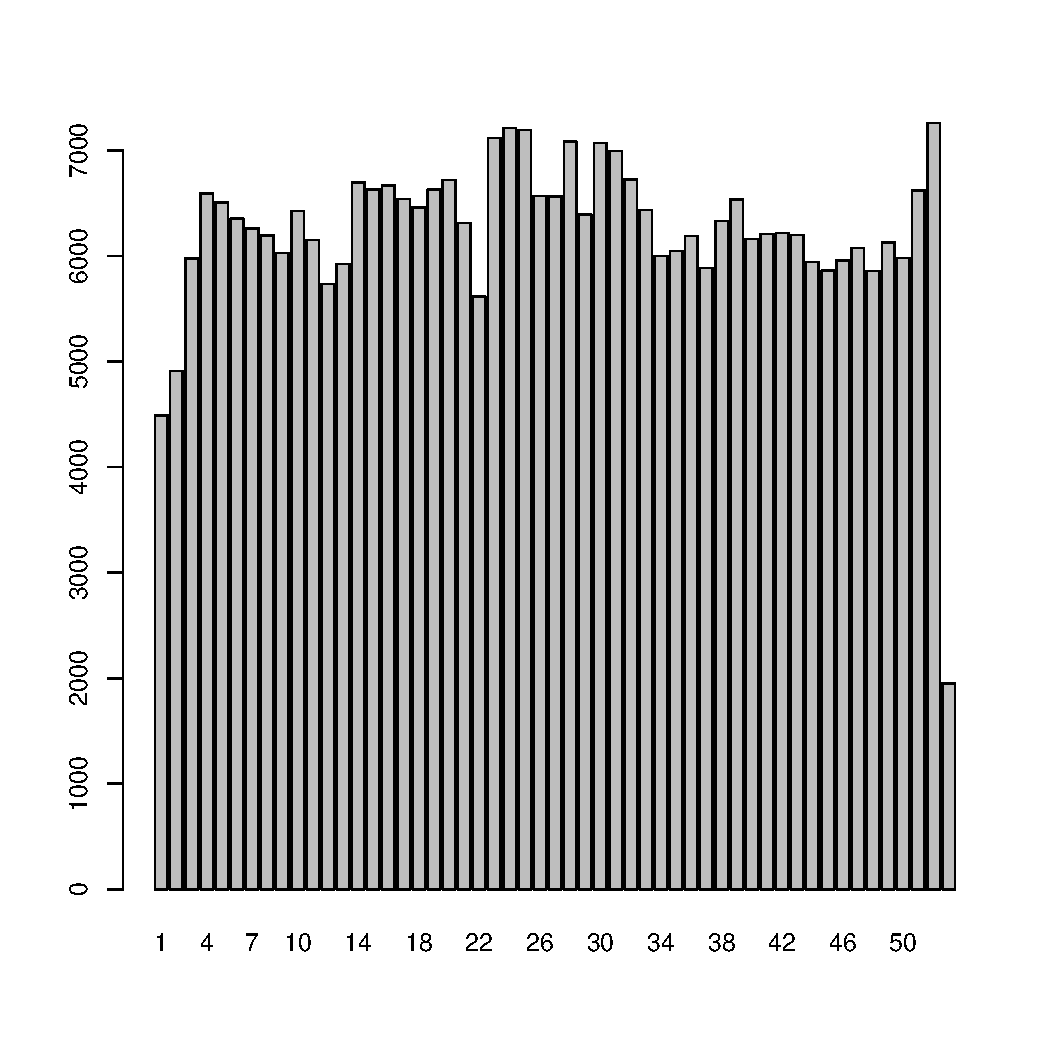
\includegraphics[width=\maxwidth]{figure/act_sem} 



\subsection*{Activité par jour de la semaine}
\begin{knitrout}
\definecolor{shadecolor}{rgb}{0.969, 0.969, 0.969}\color{fgcolor}\begin{kframe}
\begin{alltt}
\hlstd{m} \hlkwb{<-} \hlkwd{wday}\hlstd{(d1}\hlopt{$}\hlstd{ENTREE,} \hlkwc{label} \hlstd{= T)}
\hlkwd{table}\hlstd{(m)}
\end{alltt}
\begin{verbatim}
## m
##   Sun   Mon  Tues   Wed Thurs   Fri   Sat 
## 43549 45693 42301 41089 42434 42004 44697
\end{verbatim}
\begin{alltt}
\hlkwd{barplot}\hlstd{(}\hlkwd{table}\hlstd{(m),} \hlkwc{names.arg} \hlstd{=} \hlkwd{c}\hlstd{(}\hlstr{"Dim"}\hlstd{,} \hlstr{"Lun"}\hlstd{,} \hlstr{"Mar"}\hlstd{,} \hlstr{"Mer"}\hlstd{,} \hlstr{"Jeu"}\hlstd{,} \hlstr{"Ven"}\hlstd{,} \hlstr{"Sam"}\hlstd{))}
\end{alltt}
\end{kframe}
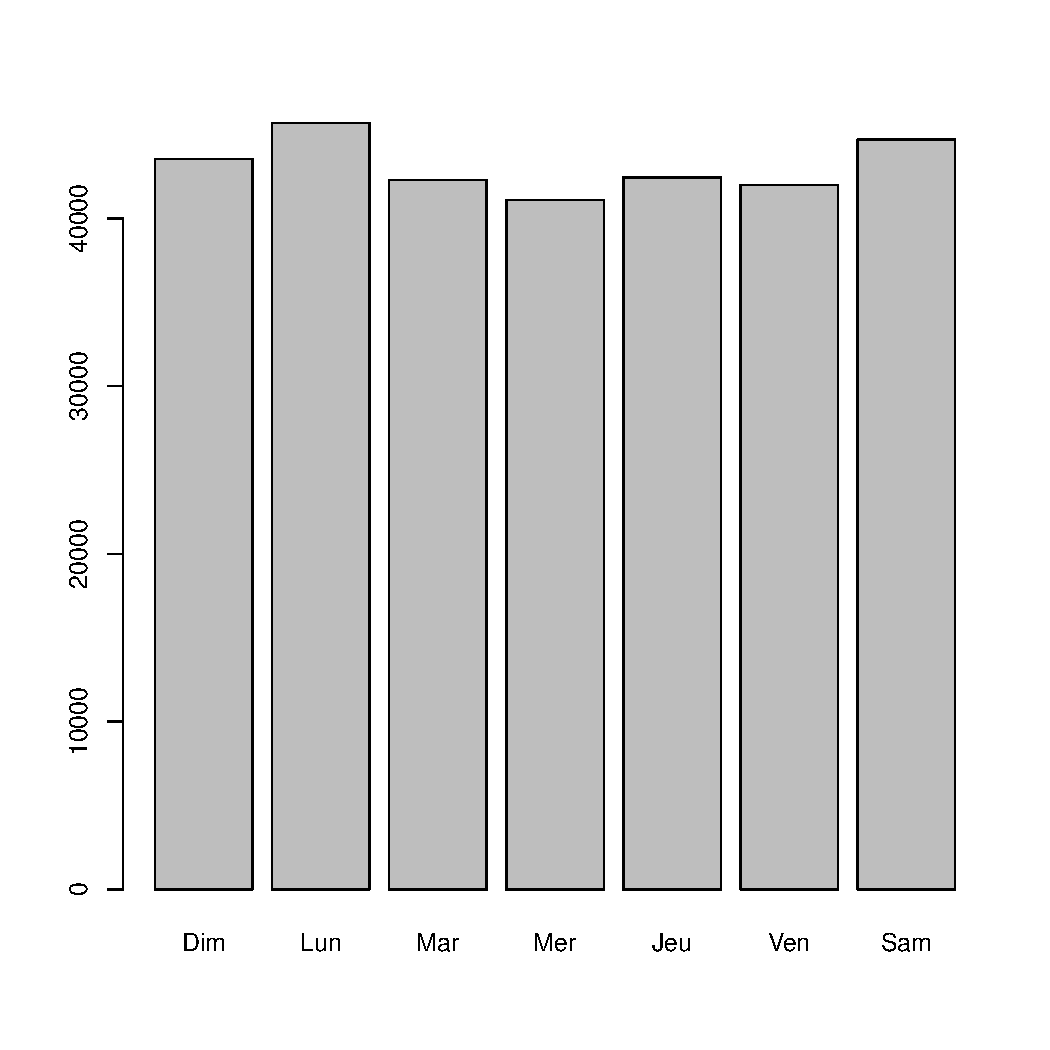
\includegraphics[width=\maxwidth]{figure/activite_semaine} 

\end{knitrout}


\subsection*{Activité horaire}
\begin{knitrout}
\definecolor{shadecolor}{rgb}{0.969, 0.969, 0.969}\color{fgcolor}
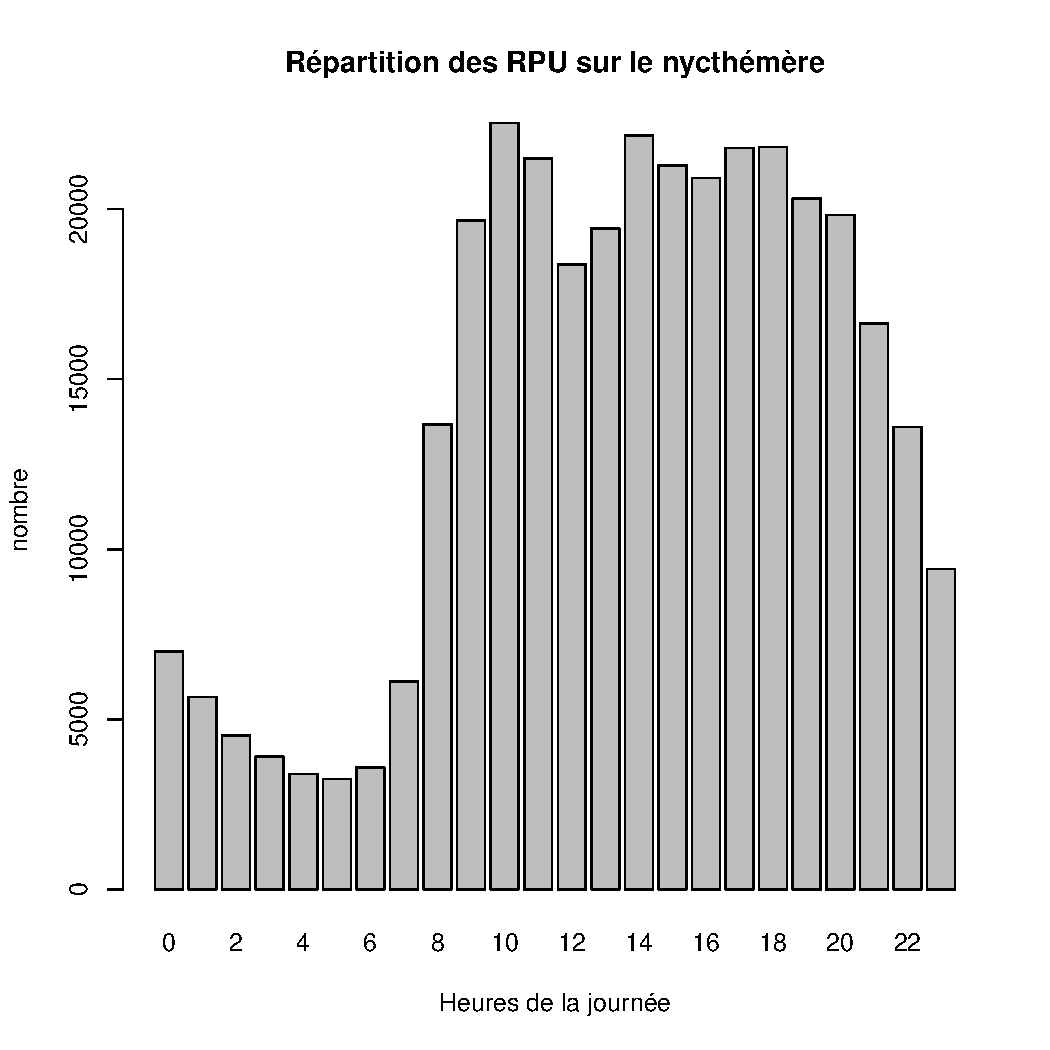
\includegraphics[width=\maxwidth]{figure/activite_heure} 

\end{knitrout}


  


\section{Passages aux urgences}

% test2.Rnw

L'activité horaire des services d'urgence en Alsace est totalement superposable à celui de l'ensemble des SU (figure \ref{passage:als} page \pageref{passage:als}). L'activité diminue fortement en nuit profonde à partir de une heure du matin pour redémarrer vers 9 heures et s'intensifier progressivement en matinée. Après un premier pic en fin de matinée, la croissance reprend pour culminer vers 19 heures, puis décroître lentement jusqu'en fin de soirée.

Ce phénomène cyclique se répète tous les jours selon un profil immuable. La projection de ces données sur un graphique en radar représentant les 24 tranches horaires (figure \ref{radar:als} page \pageref{radar:als}) montre qu'il existe trois pics d'égale amplitude à 11, 15 et 19 heures. Ce point mérite d'être analysé car s'il se confirme, cela pourrait indiquer que le pointage de 11 heures permet d'avoir une prévision sur l'intensité de la fréquentation avant la garde du soir. On peut en rapprocher le fait que la médiane des passages se situe vers 14h, c'est à dire qu'au ointage de 15 heures on peut évaluer la quantité totale de patients qui vont se présenter dans les heures qui viennent.

%----------------------------------------------------------------------------- Summary
Résumé des horaires de passage aux urgences: les données figurent dans le tableau \ref{tab:24} page \pageref{tab:24}.
\begin{kframe}


{\ttfamily\noindent\bfseries\color{errorcolor}{Error: impossible de trouver la fonction "{}xsummary"{}}}\end{kframe}


% \input{../blah.gen}
%---------------------------------------------------------------------- HISTOGRAMME

\begin{figure}
\begin{center}
\begin{knitrout}
\definecolor{shadecolor}{rgb}{0.969, 0.969, 0.969}\color{fgcolor}
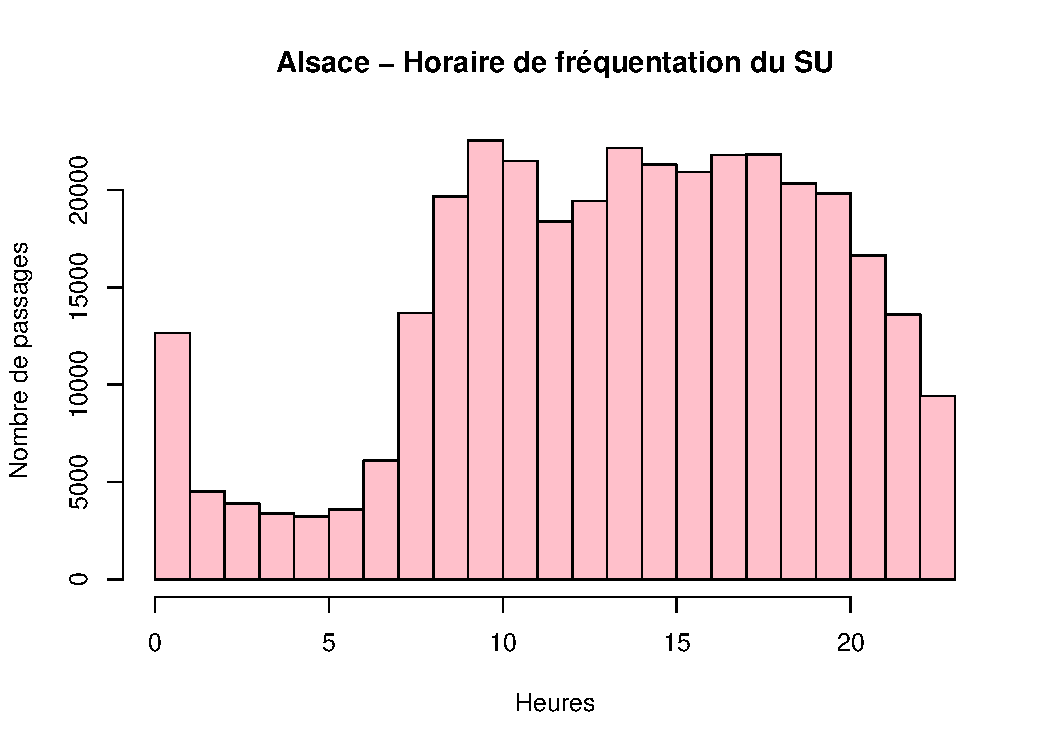
\includegraphics[width=\maxwidth]{figure/test23} 

\end{knitrout}

\end{center}
\caption{Horaires d'arrivée aux urgences en Alsace 2013}
\label{passage:als}
\end{figure}
%---------------------------------------------------------------------------- RADAR 1

\begin{figure}
\begin{center}
\begin{knitrout}
\definecolor{shadecolor}{rgb}{0.969, 0.969, 0.969}\color{fgcolor}
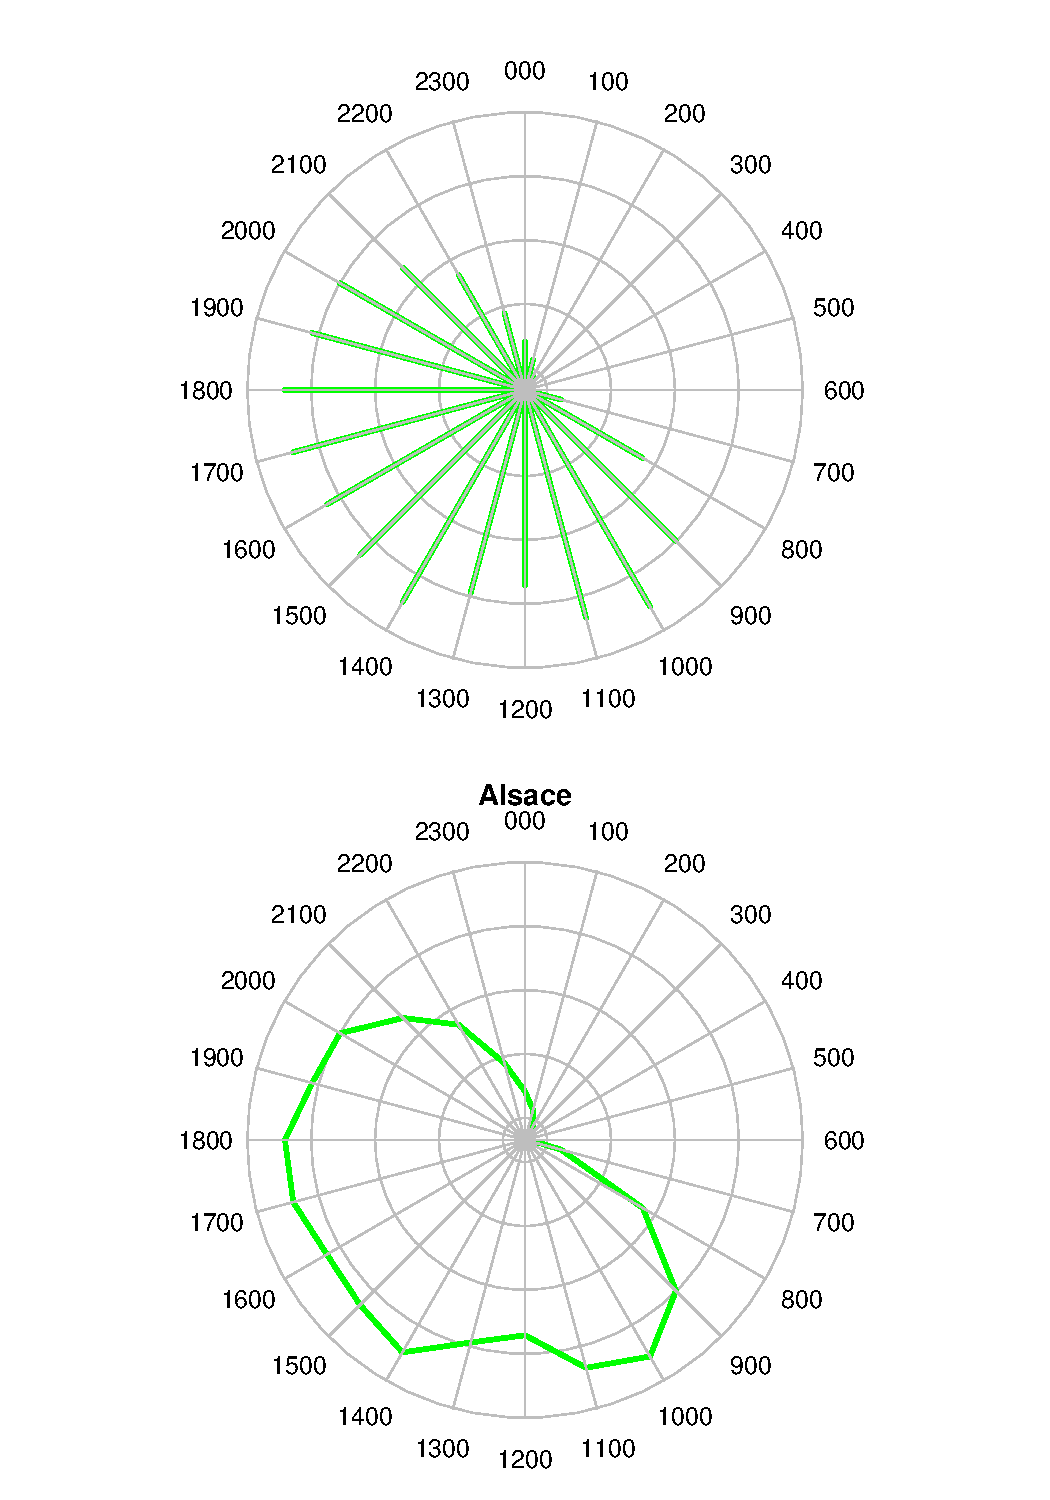
\includegraphics[width=\maxwidth]{figure/test25} 

\end{knitrout}

\end{center}
\caption{Horaires d'arrivée aux urgences en Alsace 2013}
\label{radar:als}
\end{figure}

%---------------------------------------------------------Radar HUS
\begin{figure}
\begin{center}
\begin{knitrout}
\definecolor{shadecolor}{rgb}{0.969, 0.969, 0.969}\color{fgcolor}
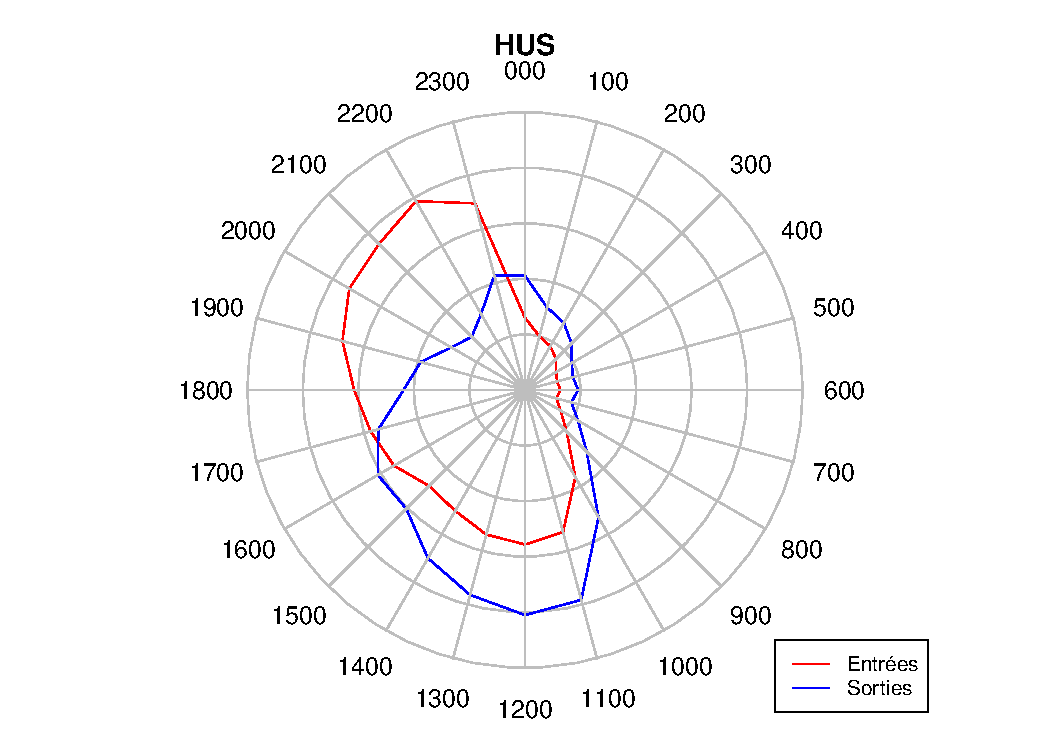
\includegraphics[width=\maxwidth]{figure/test2} 

\end{knitrout}

\end{center}
\caption{HUS: répartition des arrivées et départs aux urgences}
\label{passage:hus}
\end{figure}

%---------------------------------------------------------Radar Colmar
\begin{figure}
\begin{center}
\begin{knitrout}
\definecolor{shadecolor}{rgb}{0.969, 0.969, 0.969}\color{fgcolor}
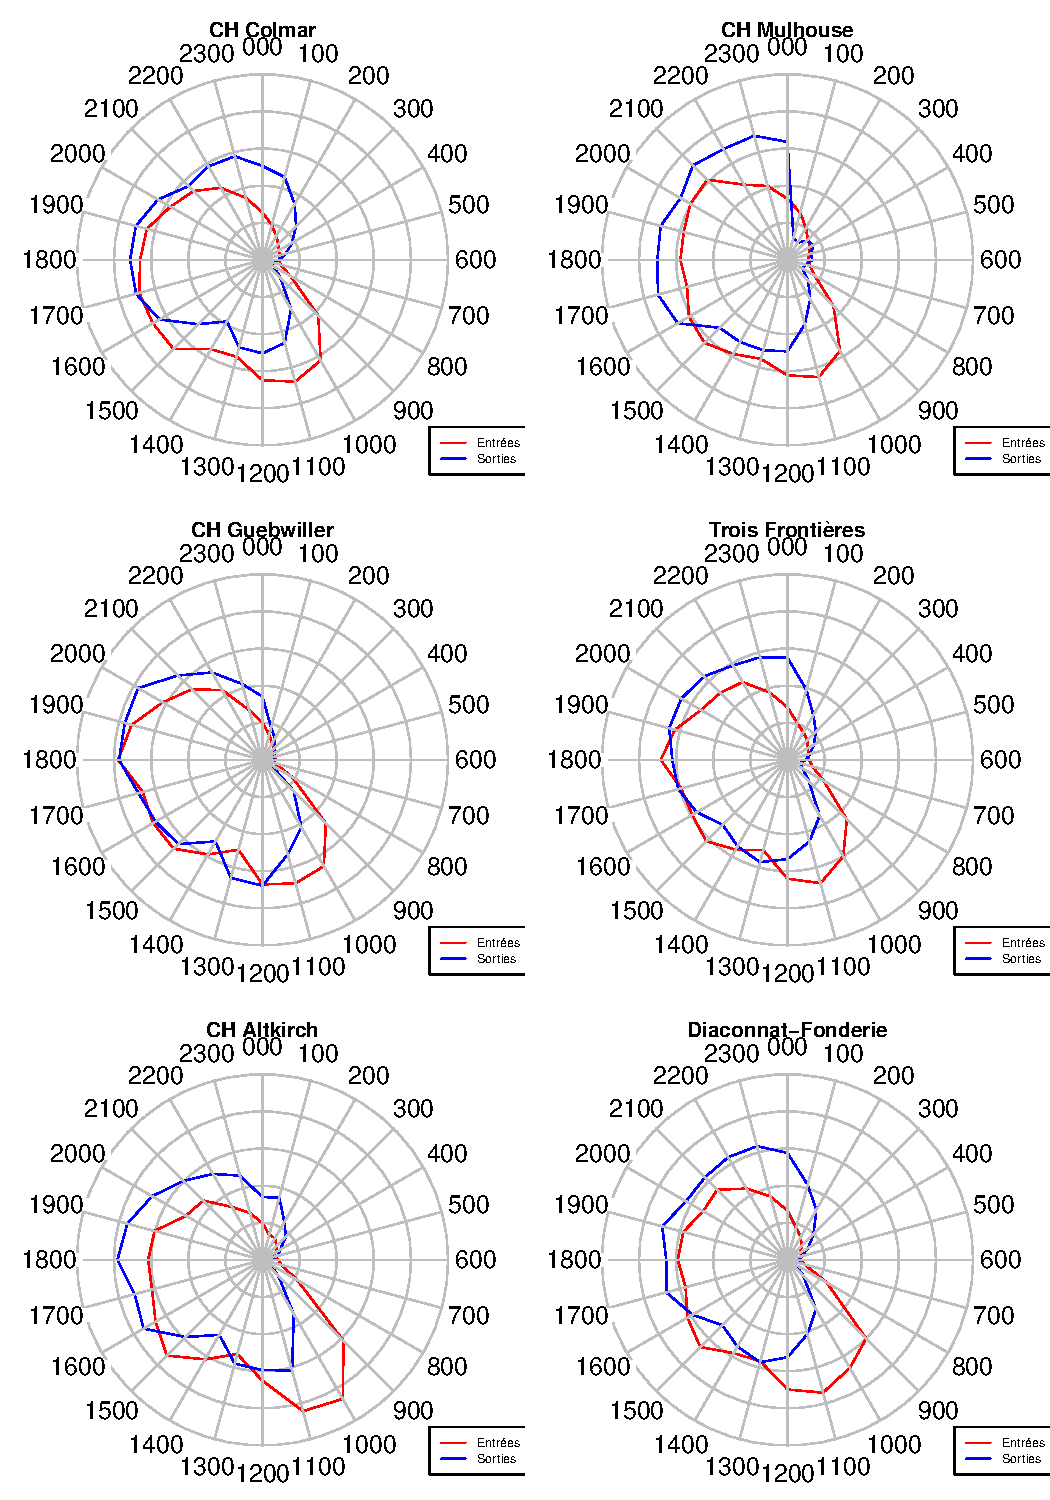
\includegraphics[width=\maxwidth]{figure/test26} 

\end{knitrout}

\end{center}
\caption{Secteurs 3 et 4: répartition des arrivées et départs aux urgences}
\label{passage:col}
\end{figure}

\begin{figure}
\begin{center}
\begin{knitrout}
\definecolor{shadecolor}{rgb}{0.969, 0.969, 0.969}\color{fgcolor}
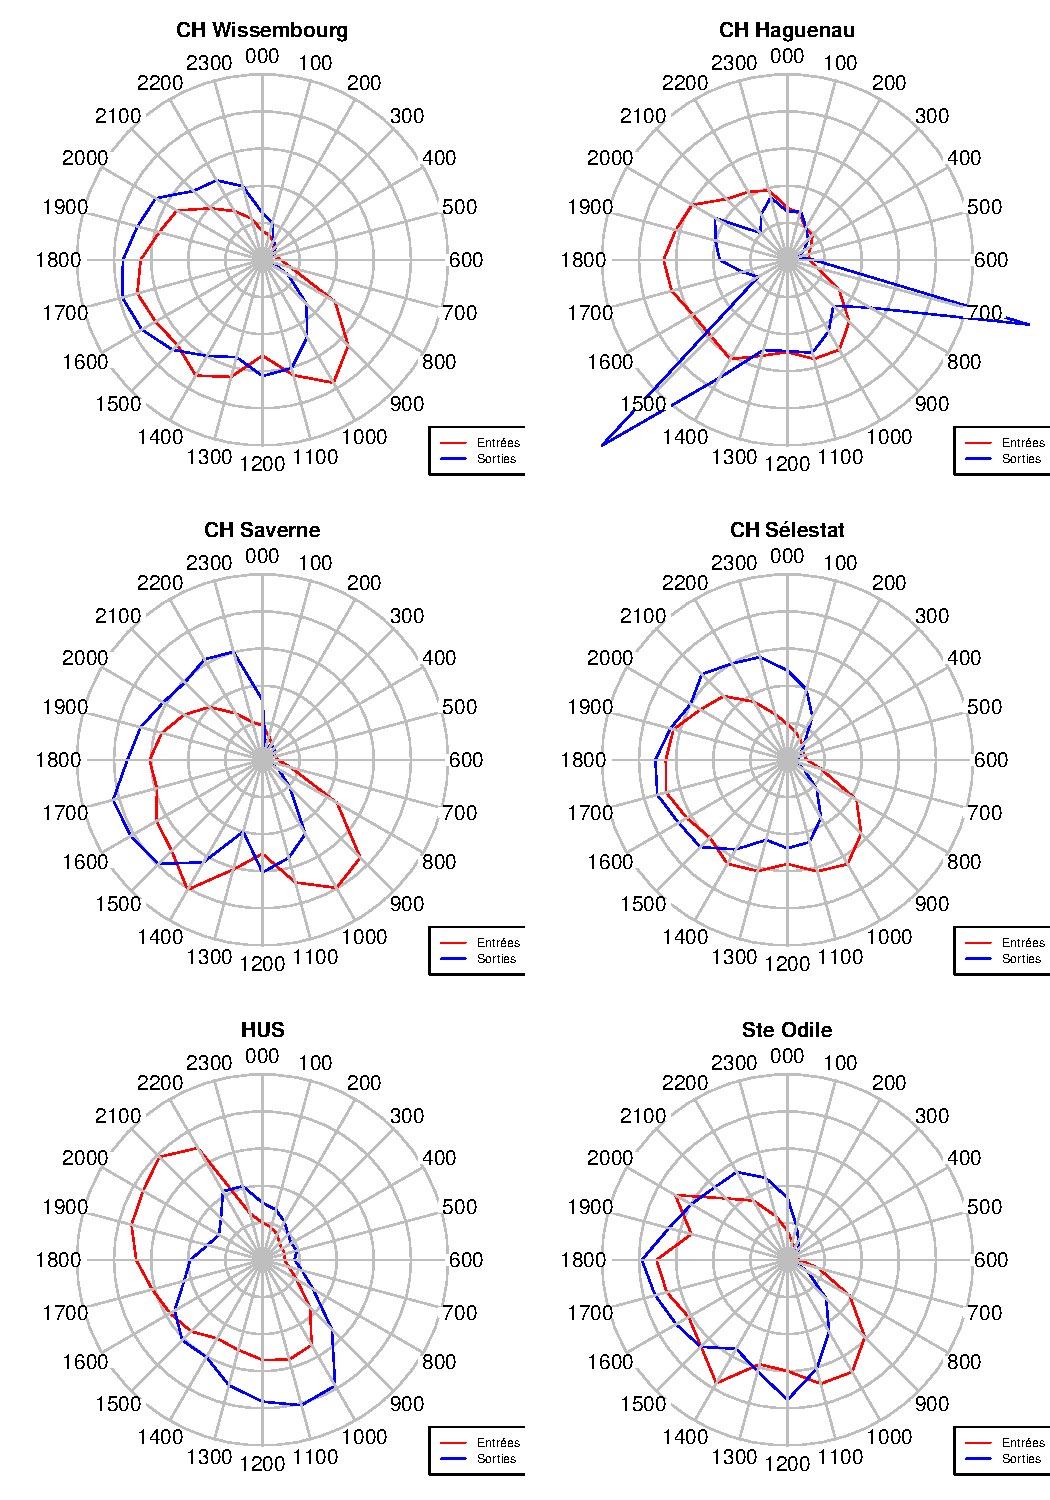
\includegraphics[width=\maxwidth]{figure/test27} 

\end{knitrout}

\end{center}
\caption{Secteurs 1 et 2: répartition des arrivées et départs aux urgences}
\label{passage:secteur12}
\end{figure}



\subsection{Passages par tranches d'âge}

% tranche-age.Rnw

% latex table generated in R 3.0.2 by xtable 1.7-1 package
% Sat Dec 21 11:32:28 2013
\begin{table}[ht]
\centering
\begin{tabular}{rr}
  \hline
 & a \\ 
  \hline
Moins de 1 an & 7865 \\ 
  De 1 à 15 ans & 54374 \\ 
  De 15 à 75 ans & 192994 \\ 
  de 75 à 85 ans & 27253 \\ 
  Plus de 85 ans & 19241 \\ 
   \hline
\end{tabular}
\caption[Répartition des RPU par tranches d'age]{Répartition des RPU par tranches d'age} 
\label{tab:tranche}
\end{table}

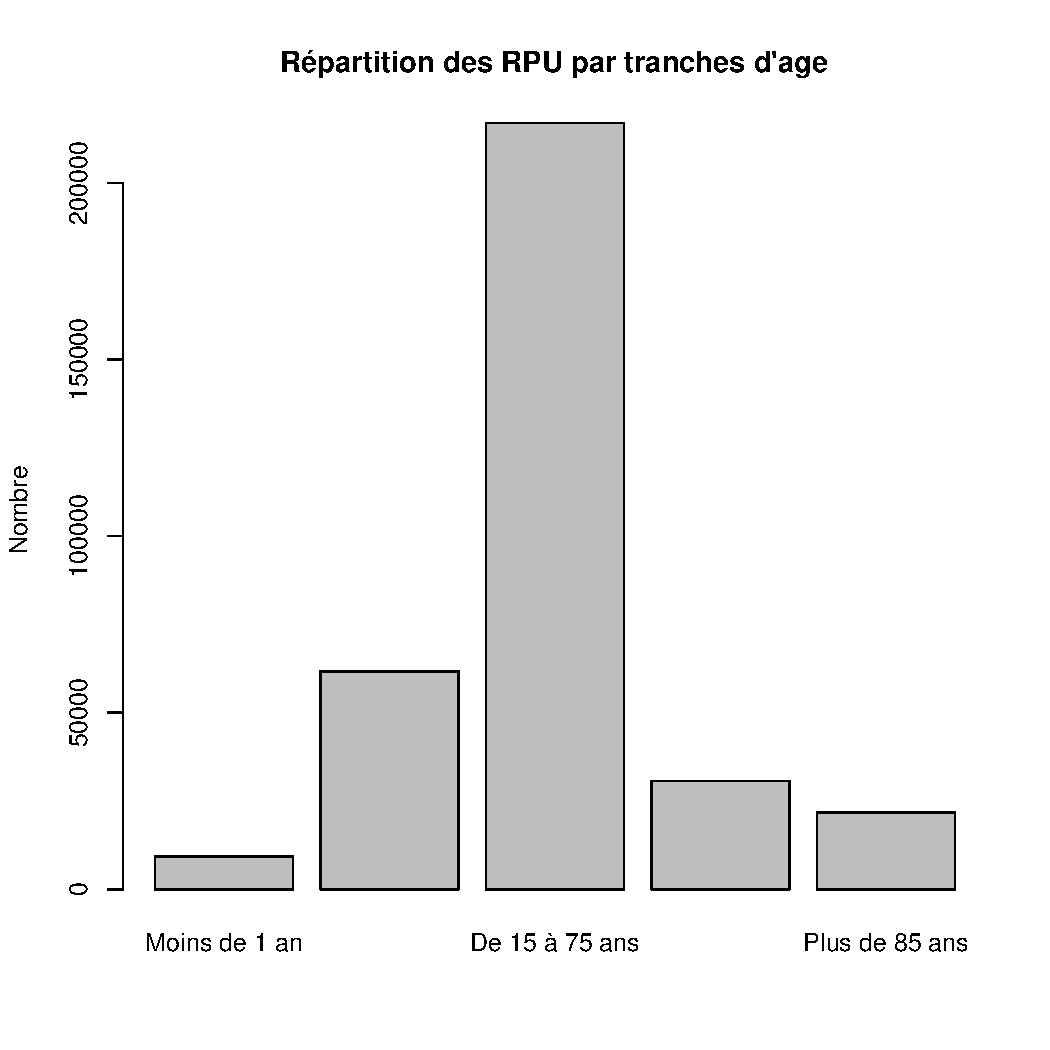
\includegraphics[width=\maxwidth]{figure/tranche} 




\newpage
\chapter{Motif de consultation}

% motif.Rnw

\index{motif de consultation}

Le motif de consultation est l'un des items les plus mal renseigné. Cela est du en partie à l'absence de règles formelles concernant la saisie de cet élément. Une recommandation du ministère de la santé (juin 2013 \cite{12,13}) demande que le thésaurus 2013 de la SFMU \cite{9} soit utilisé.

Le thésaurus est présenté sous la formed'un fichier Excel. L'onglet \emph{recours} liste environ \emph{150} motifs de recours aux urgences avec leur correspondance CIM10, répartis en 17 groupes. Aucune méthode n'est parfaite mais cette page constitue une bonne base d'harmonisation des données.


% latex table generated in R 3.0.2 by xtable 1.7-1 package
% Sat Dec 21 11:32:28 2013
\begin{table}[ht]
\centering
\begin{tabular}{rrrrrrrrrrrrr}
  \hline
 & X3Fr & Alk & Col & Dia & Geb & Hag & Hus & Mul & Odi & Sel & Wis & Sav \\ 
  \hline
1 & 7.47 & 22.92 & 100.00 & 95.54 & 0.04 & 13.53 & 0.00 & 83.22 & 94.81 & 98.05 & 99.70 & 41.87 \\ 
   \hline
\end{tabular}
\caption[motif de consultation]{Taux de réponse à l'item motif de consultation selon le services d'urgence} 
\label{lab:motif}
\end{table}

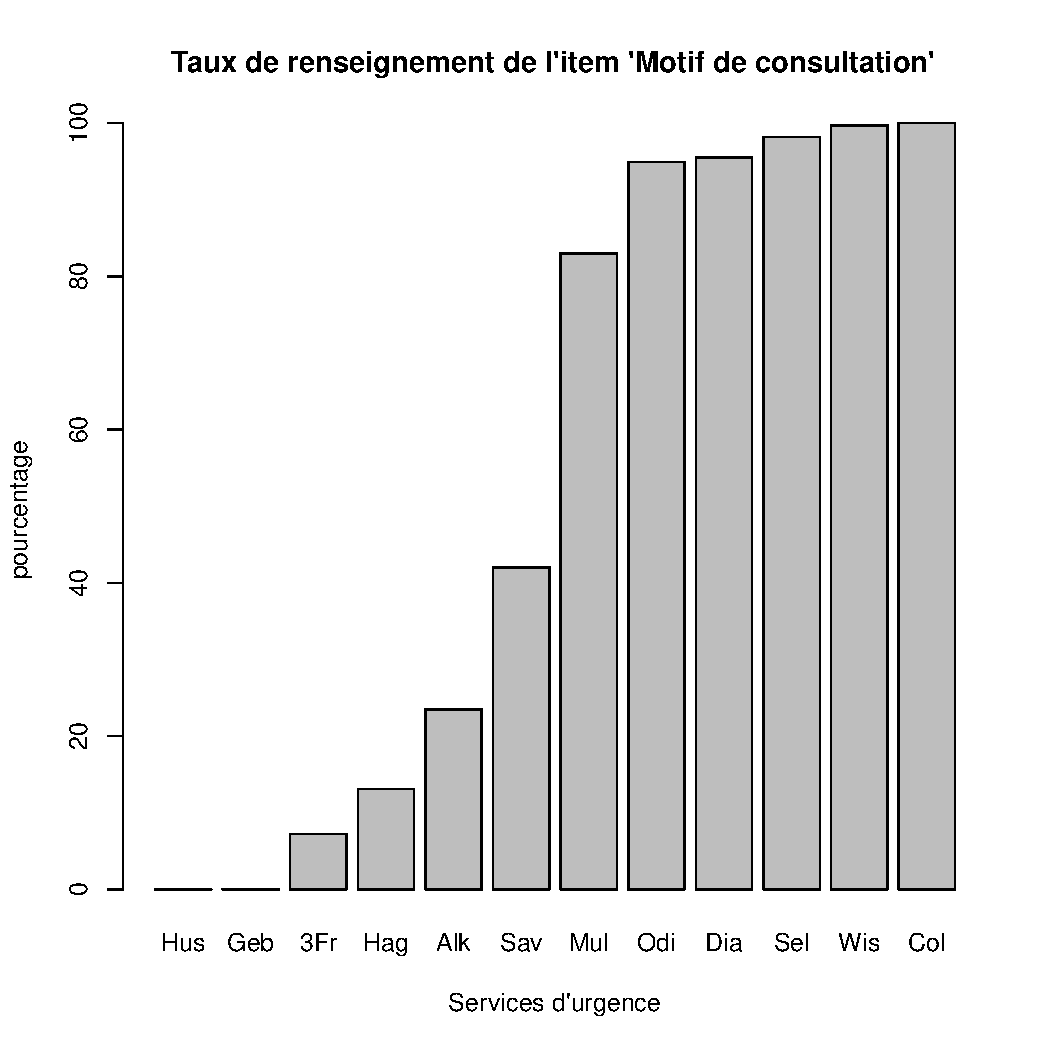
\includegraphics[width=\maxwidth]{figure/motifss1} 

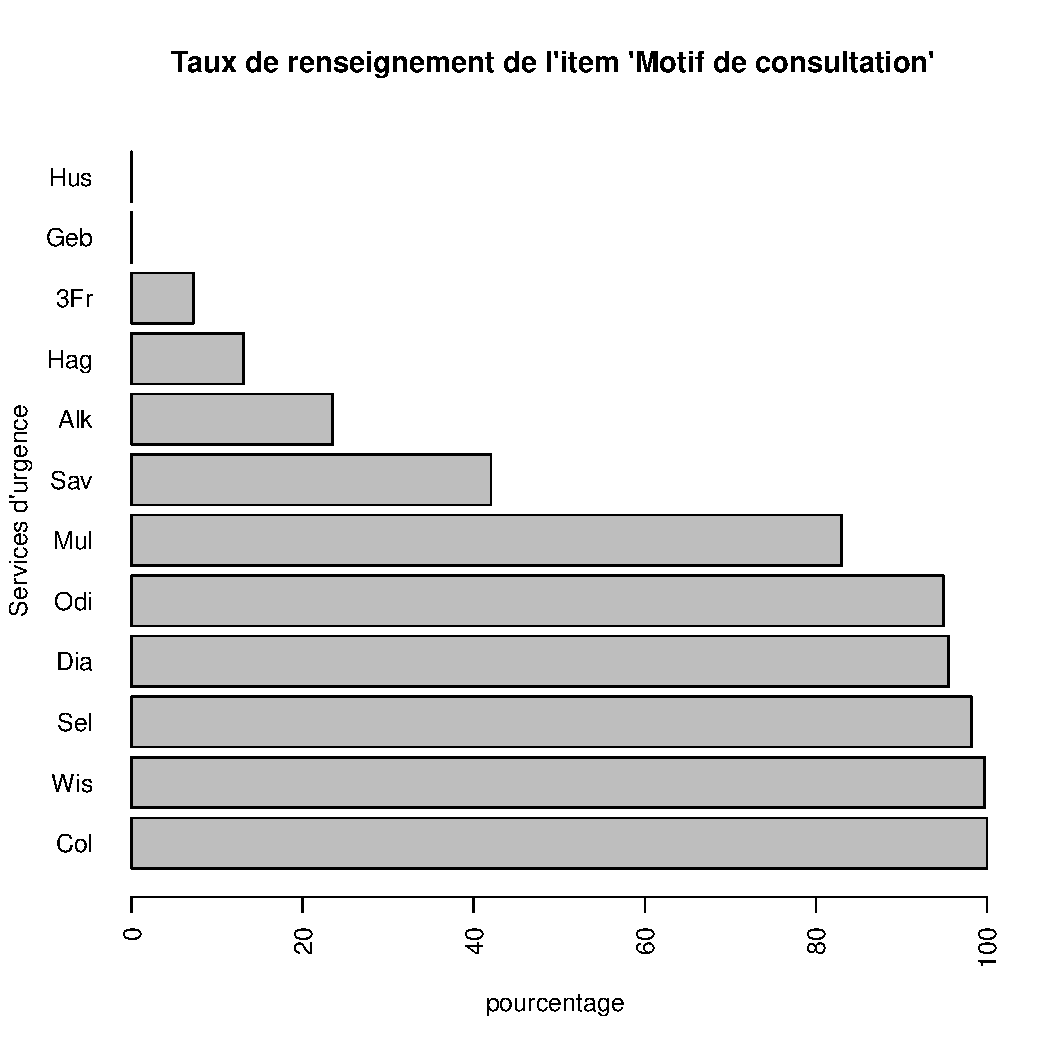
\includegraphics[width=\maxwidth]{figure/motifss2} 



\index{exhaustivité@motif}
Le motif de consultation nest pas renseigné dans 54.76 \% des cas (table \ref{lab:motif}).

Seuls six établissements ont un taux d'exhaustivité supérieur à 80\% pour cette rubrique.

Cependant seuls quelques établissements saisissent cette information sous forme normalisée qui permet de l'exploiter. Dans les autres cas il s'agit de codes propre à l'établissement ou de texte libre inexploitable.

Données non renseignées:
\begin{itemize}
  \item Guebwiller
  \item HUS
  \item Ste Anne
  \item Tann
\end{itemize}

Données renseignées mais inexploitables:
\begin{itemize}
  \item Colmar
  \item Sélestat
  \item Haguenau
\end{itemize}

Données renseignées, exploitables mais à mettre en conformité avec le thésaurus:
\begin{itemize}
  \item Mulhouse
  \item Wissembourg
  \item Altkirch (exhaustivité)
  \item Saverne
  \item Ste Odile
  \item Diaconnat Fonderie
  \item Trois Frontières
\end{itemize}


\newpage
\chapter{Modalité d'admission}

% modalites.Rnw
% modalités d'admission MODE_ENTREE

\index{Mode d'entrée}

\section*{Origine des patients}
% REMARQUE dans environ 300 dossiers du mois de juin, l'item transfert est écrit "transfe  rt" ce qui nécessite un recodage.

L'immense majorité des patients provient du domicile ou son équivalent. Une très faible part des passages aux urgences sont le fait de transferts d'autres établissements ou de mutations en provenance d'autres services du même établissement.


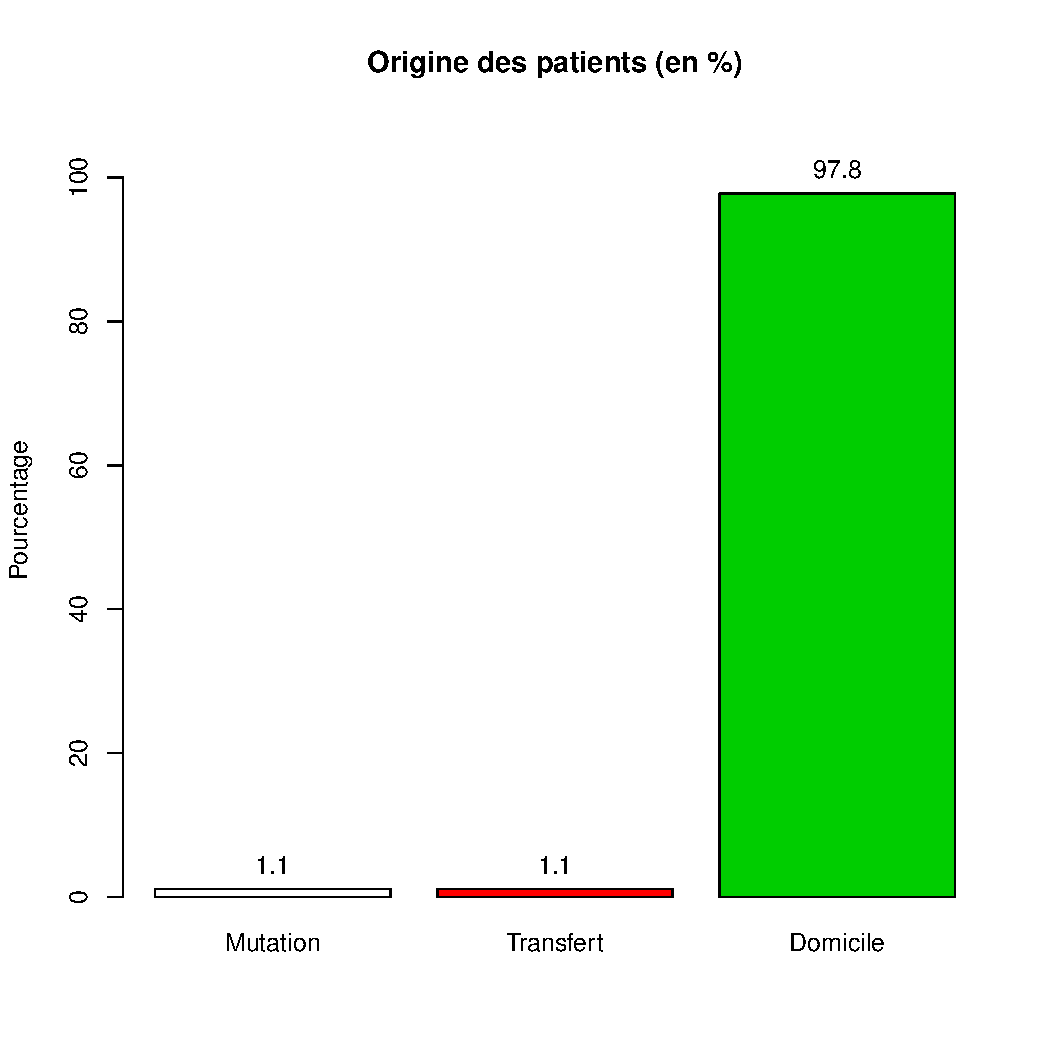
\includegraphics[width=\maxwidth]{figure/mode_entree} 
% latex table generated in R 3.0.2 by xtable 1.7-1 package
% Sat Dec 21 11:32:29 2013
\begin{table}[ht]
\centering
\begin{tabular}{rrrr}
  \hline
 & Frequency &   \%(NA+) &   \%(NA-) \\ 
  \hline
Mutation & 3277.00 & 1.10 & 1.20 \\ 
  Transfert & 2908.00 & 1.00 & 1.10 \\ 
  Domicile & 265384.00 & 87.90 & 97.70 \\ 
  NA's & 30198.00 & 10.00 & 0.00 \\ 
    Total & 301767.00 & 100.00 & 100.00 \\ 
   \hline
\end{tabular}
\caption[Origine des patients]{Origine des patients. Les deux colonnes de droite mesurent l'origine (en pourcentage) selon que l'on prenne en compte ou non les valeurs manquantes. } 
\label{origine}
\end{table}



Dans 10 \% des cas, l'origine du patient n'est pas précisée.

\section*{Mode de transport}
\index{Mode de transport}

La grande majorité des patients arrivent aux urgences par leurs propres moyens (PERSO). Lorsqu'ils font appel à un tiers, il s'agit le plus souvent d'une ambulance privée (AMBU), puis du SDIS (AMBU). Les transports par un vecteur médicalisé (SMUR) ou héliporté (HELI) sont rares. Enfin l'utilisation des forces de l'ordre (FO) comme moyen de transport reste marginale.


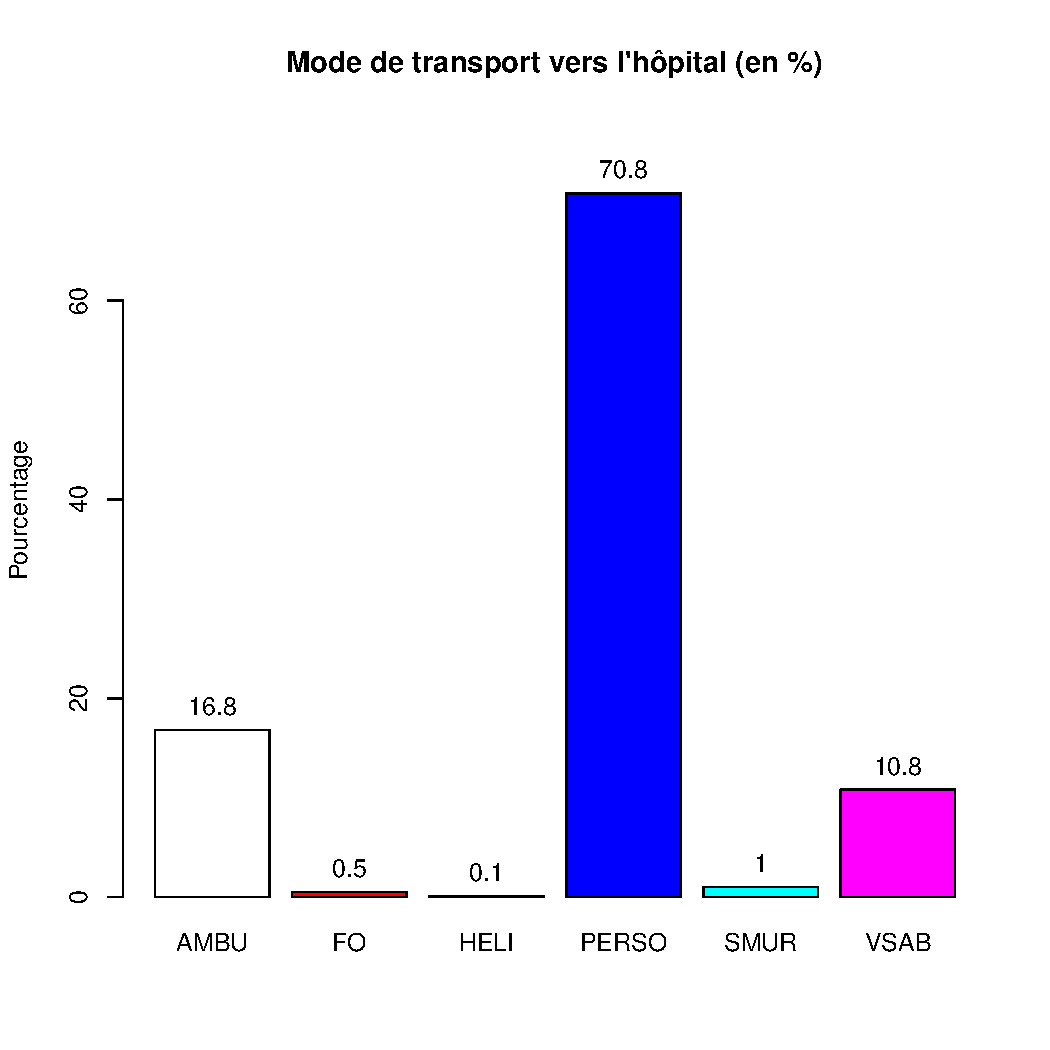
\includegraphics[width=\maxwidth]{figure/transport} 
% latex table generated in R 3.0.2 by xtable 1.7-1 package
% Sat Dec 21 11:32:29 2013
\begin{table}[ht]
\centering
\begin{tabular}{rrrr}
  \hline
 & Frequency &   \%(NA+) &   \%(NA-) \\ 
  \hline
AMBU & 39501.00 & 13.10 & 17.10 \\ 
  FO & 1269.00 & 0.40 & 0.50 \\ 
  HELI & 186.00 & 0.10 & 0.10 \\ 
  PERSO & 162761.00 & 53.90 & 70.40 \\ 
  SMUR & 2378.00 & 0.80 & 1.00 \\ 
  VSAB & 24962.00 & 8.30 & 10.80 \\ 
  NA's & 70710.00 & 23.40 & 0.00 \\ 
    Total & 301767.00 & 100.00 & 100.00 \\ 
   \hline
\end{tabular}
\caption[Moyens de transport]{Moyens de transport utilisés pour se rendre à l'hôpital. Les deux colonnes de droite mesurent la fréquence du moyen utilise (en pourcentage) selon que l'on prenne en compte ou non les valeurs manquantes. } 
\label{transport}
\end{table}



Dans 23.4 \% des cas, le moyen de transport utilisé par le patient pour rejoindre l'hôpial n'est pas précisé.

\section*{Origine géographique}



Les patients consultant aux urgences sont majoritairement issus de la région Alsace. Mais l'origine est très diverse, aussi bien en provenance des autres départements français qu'hors de France:
% \begin{itemize}
%   \item Alsace: cp_als (\Sexpr(round(cp_als*100/n,2) \%))
%   \item hors Alsace: cp_hals
%   \item dont hors de France: cp_monde
% \end{itemize}



\newpage
\chapter{Durée de passage}

% duree_passage.Rnw

La durée de passage est le temps compris entre la date d'entrée et celle de sortie. Il s'agit d'une durée de transit total. Les données transmises par les RPU ne permettent pas de calculer les temps d'attente.

\subsection{Cas général}




La dispersion des durées de passage est très importante, variant de -247 à \np{9870} minutes. Les valeurs négatives sont considérées comme des valeurs manquantes. 
Finalement \ensuremath{2.7627\times 10^{4}} ne sont pas renseignées (exhaustivité de -8.16 \% des RPU). 
La durée de passage moyenne est de 163 minutes (ecart-type 197.97 minutes)
Une transformation logarithmique des données permet de mieux représenter l'histogramme des durées de passage. 

\begin{figure}[ht!]
 \centering
\begin{knitrout}
\definecolor{shadecolor}{rgb}{0.969, 0.969, 0.969}\color{fgcolor}
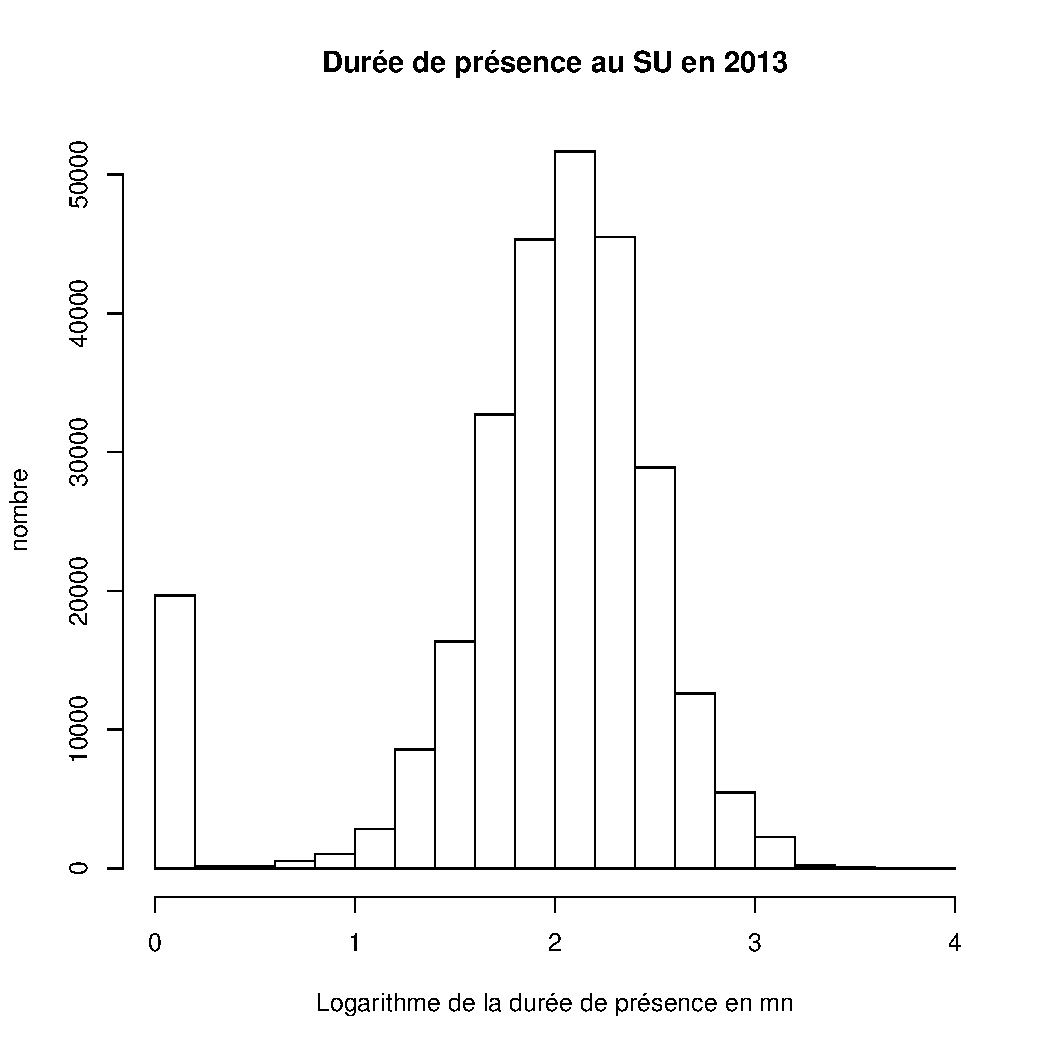
\includegraphics[width=\maxwidth]{figure/log_passages} 

\end{knitrout}

 \caption{Durée de passage (log 10)}
\end{figure}

la transformation log produit une courbe normale où lamajorité des consultants ont une durée de présence comprise entre 10 et 1000 minutes (environ 17 heures). On nettoie les données en supprimant les enregistrements où presence = NA, puis on forme 3 sous-groupes:
\begin{itemize}
  \item a moins de 10 mn
  \item b de 10 à 1000 mn
  \item c plus de 1000 mn
\end{itemize}

\begin{knitrout}
\definecolor{shadecolor}{rgb}{0.969, 0.969, 0.969}\color{fgcolor}\begin{kframe}
\begin{verbatim}
##    Min. 1st Qu.  Median    Mean 3rd Qu.    Max. 
##      10      65     119     164     211    1000
\end{verbatim}
\end{kframe}
\end{knitrout}


Les durées de présences inférieures à 10 minutes proviennent à plus de 90\% des HUS (Erreur logicielle signalée au CRIH):
\begin{knitrout}
\definecolor{shadecolor}{rgb}{0.969, 0.969, 0.969}\color{fgcolor}\begin{kframe}
\begin{alltt}
\hlcom{# Origine despatients restants moins de 10 mn: ils proviennent}
\hlcom{# majoritairement des HUS:}
\hlstd{a} \hlkwb{<-} \hlstd{d2[d2}\hlopt{$}\hlstd{presence} \hlopt{<} \hlnum{10}\hlstd{,} \hlstr{"FINESS"}\hlstd{]}
\hlkwd{rbind}\hlstd{(}\hlkwd{table}\hlstd{(a),} \hlkwd{round}\hlstd{(}\hlkwd{prop.table}\hlstd{(}\hlkwd{table}\hlstd{(a))} \hlopt{*} \hlnum{100}\hlstd{,} \hlnum{2}\hlstd{))}
\end{alltt}
\begin{verbatim}
##         3Fr   Alk   Col Dia   Geb    Hag      Hus    Mul   Odi   Sel
## [1,] 164.00 62.00 257.0 213 99.00 140.00 19576.00 408.00 95.00 27.00
## [2,]   0.77  0.29   1.2   1  0.46   0.66    91.78   1.91  0.45  0.13
##         Wis    Sav
## [1,] 142.00 147.00
## [2,]   0.67   0.69
\end{verbatim}
\begin{alltt}
\hlcom{# Plus de 90% proviennent des HUS}
\end{alltt}
\end{kframe}
\end{knitrout}


Finalement, on conserve le groupe $b$ qui regroupe la majorité (91.29\%) des patients. On trouve dans ce groupe une durée de présence de 164 minutes (écart-type 148.331 minutes, médiane 119).

\begin{figure}[ht!]
 \centering
\begin{knitrout}
\definecolor{shadecolor}{rgb}{0.969, 0.969, 0.969}\color{fgcolor}
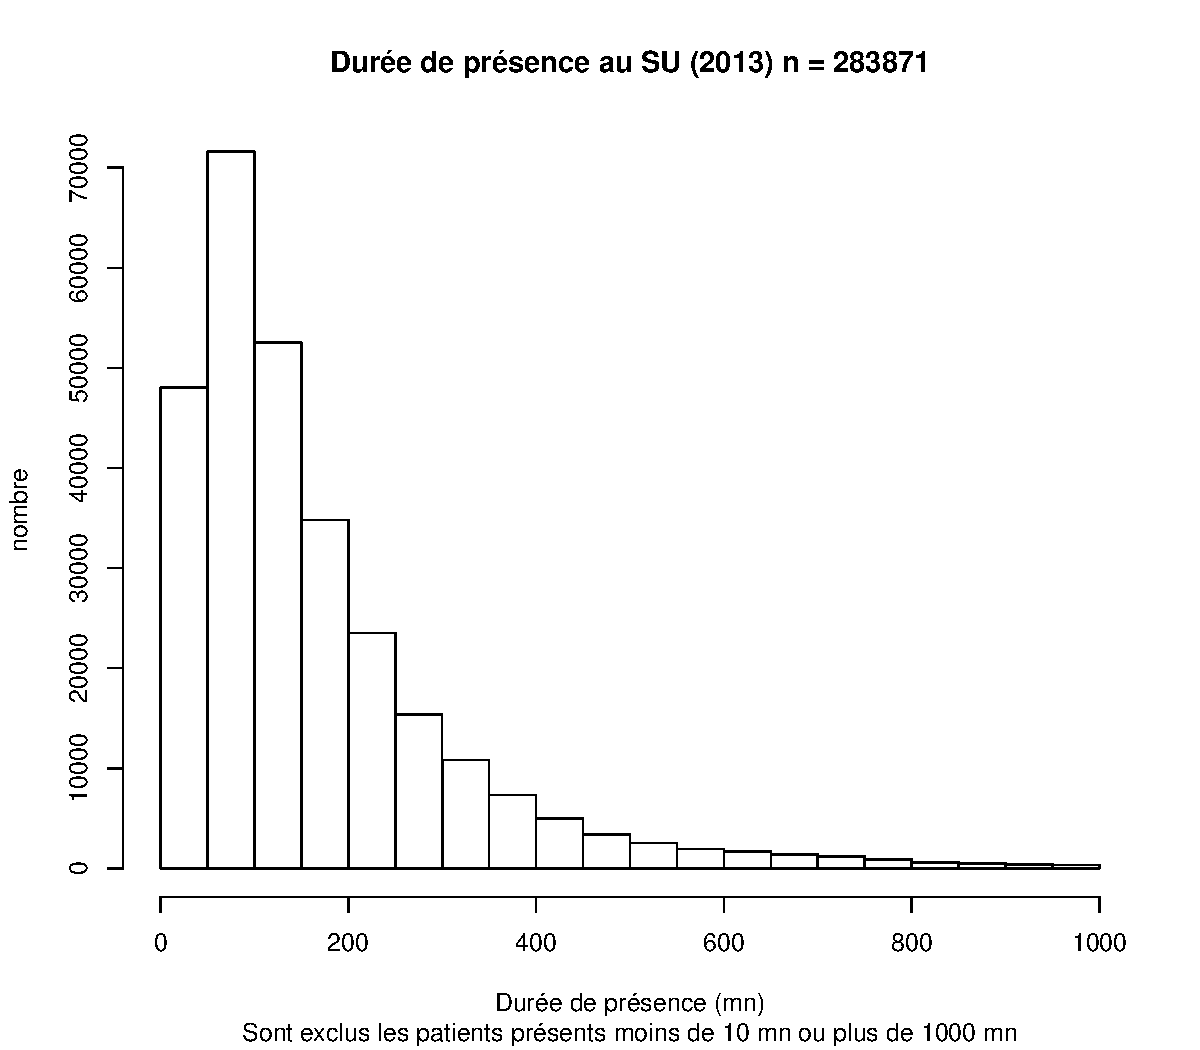
\includegraphics[width=\maxwidth]{figure/passages_clean_hist} 

\end{knitrout}

 \caption{Durée de passage aux urgences}
\end{figure}

\subsection{Moyenne des durées de passages par jour}




\begin{figure}[ht!]
 \centering
\begin{knitrout}
\definecolor{shadecolor}{rgb}{0.969, 0.969, 0.969}\color{fgcolor}
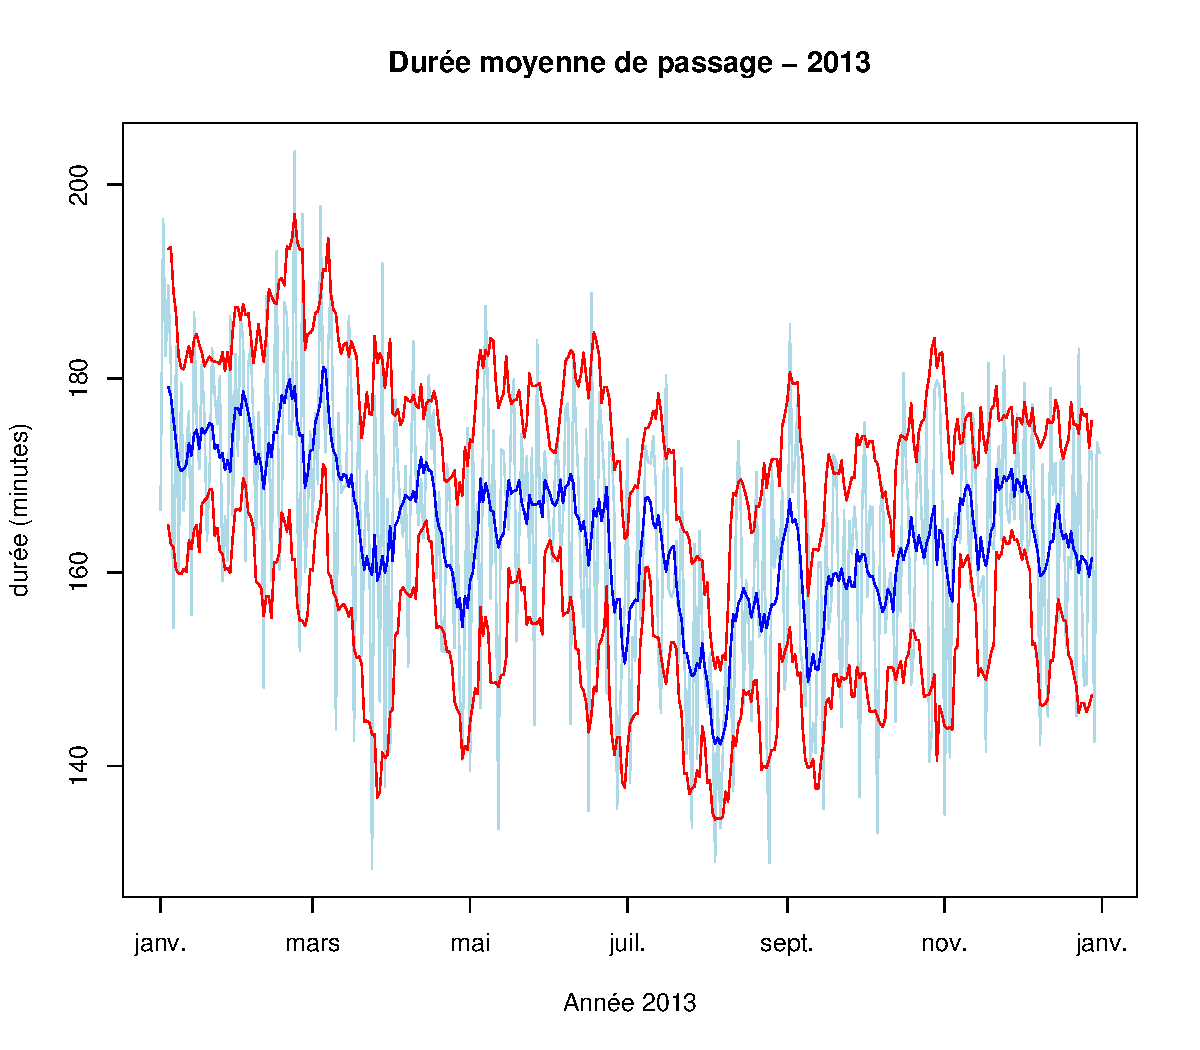
\includegraphics[width=\maxwidth]{figure/graphe_duree_moyenne_passage} 

\end{knitrout}

 \caption{Durée moyenne de passage aux urgences en 2013}
\end{figure}



\subsection{Cas particulier de Selestat}

\begin{knitrout}
\definecolor{shadecolor}{rgb}{0.969, 0.969, 0.969}\color{fgcolor}\begin{kframe}


{\ttfamily\noindent\color{warningcolor}{\#\# Warning: All formats failed to parse. No formats found.}}\begin{verbatim}
##    Min. 1st Qu.  Median    Mean 3rd Qu.    Max.    NA's 
##       1      86     137     162     216     974     627
\end{verbatim}
\end{kframe}
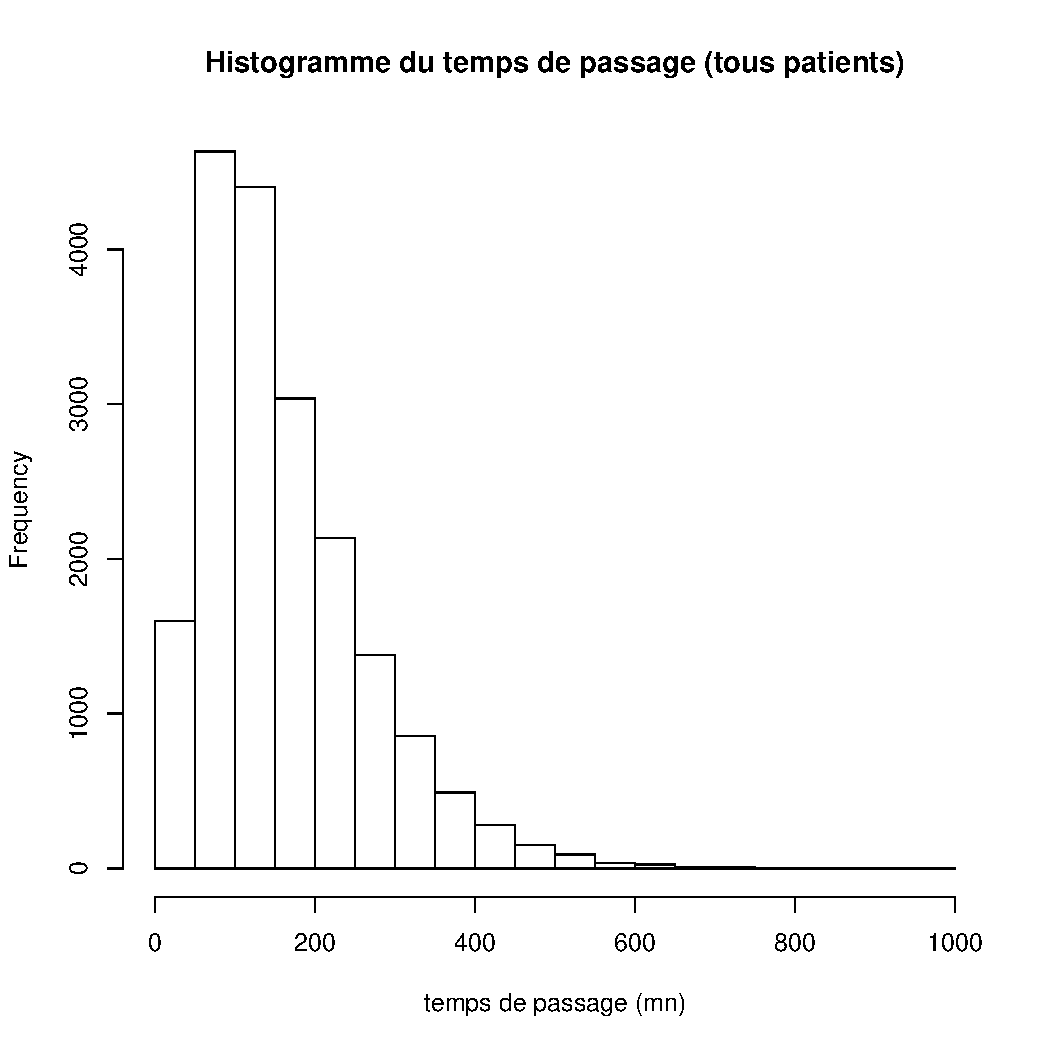
\includegraphics[width=\maxwidth]{figure/passage} 

\end{knitrout}


% RPU_2013_analyse à partir de la ligne 382

\section*{Selon l'heure}

Une période de 24 heures est habituellement divisée de la manière suivante:
\begin{enumerate}
  \item \emph{journée} de 8 heures à 20 heures
  \item \emph{soirée} de 20 heures à minuit
  \item  \emph{nuit profonde} de 0 heures à 8 heures
\end{enumerate}




\begin{knitrout}
\definecolor{shadecolor}{rgb}{0.969, 0.969, 0.969}\color{fgcolor}\begin{kframe}
\begin{verbatim}
## nuit profonde       journée        soirée          NA's 
##         38975        221056         35492          6244
\end{verbatim}
\end{kframe}
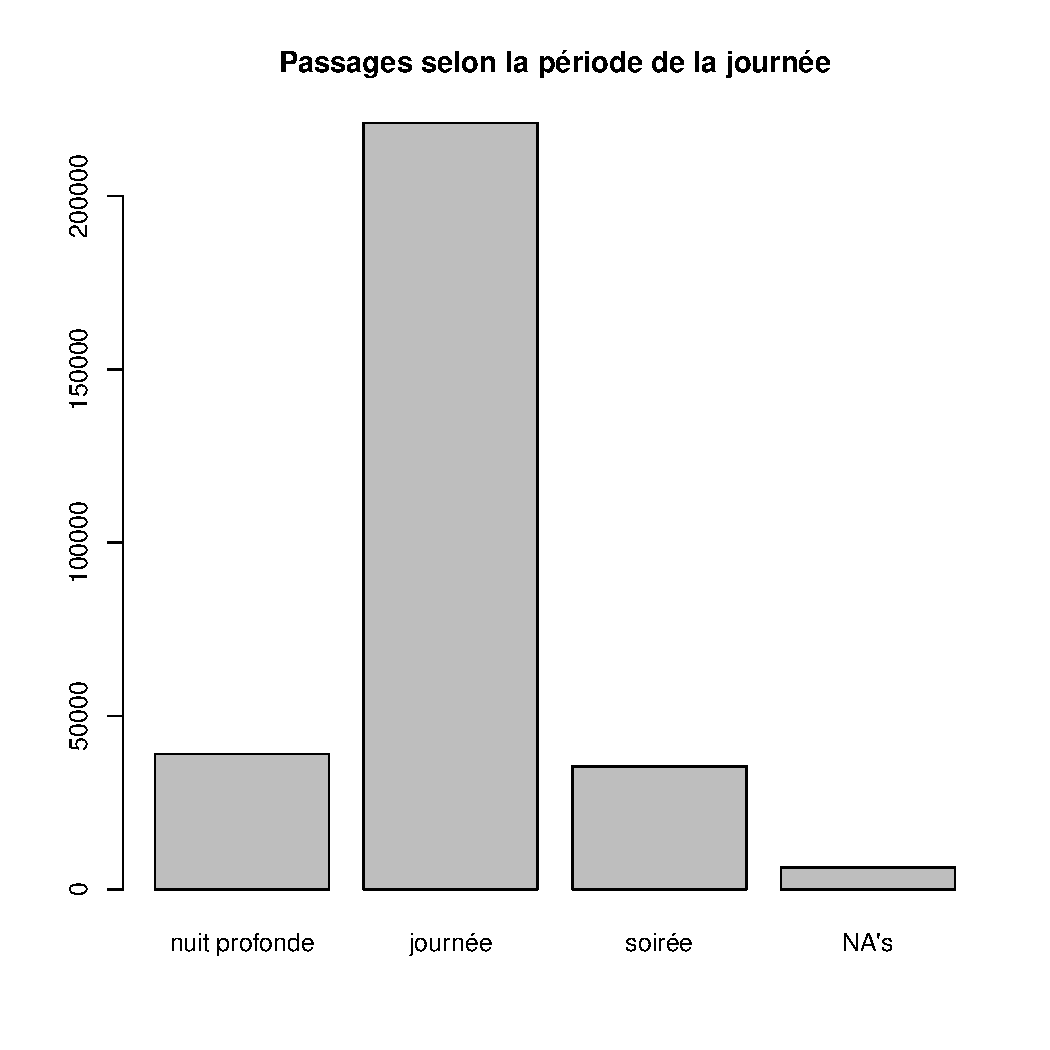
\includegraphics[width=\maxwidth]{figure/duree_heure1} 
\begin{kframe}\begin{verbatim}
## nuit profonde       journée        soirée 
##         173.2         161.1         163.1
\end{verbatim}
\end{kframe}
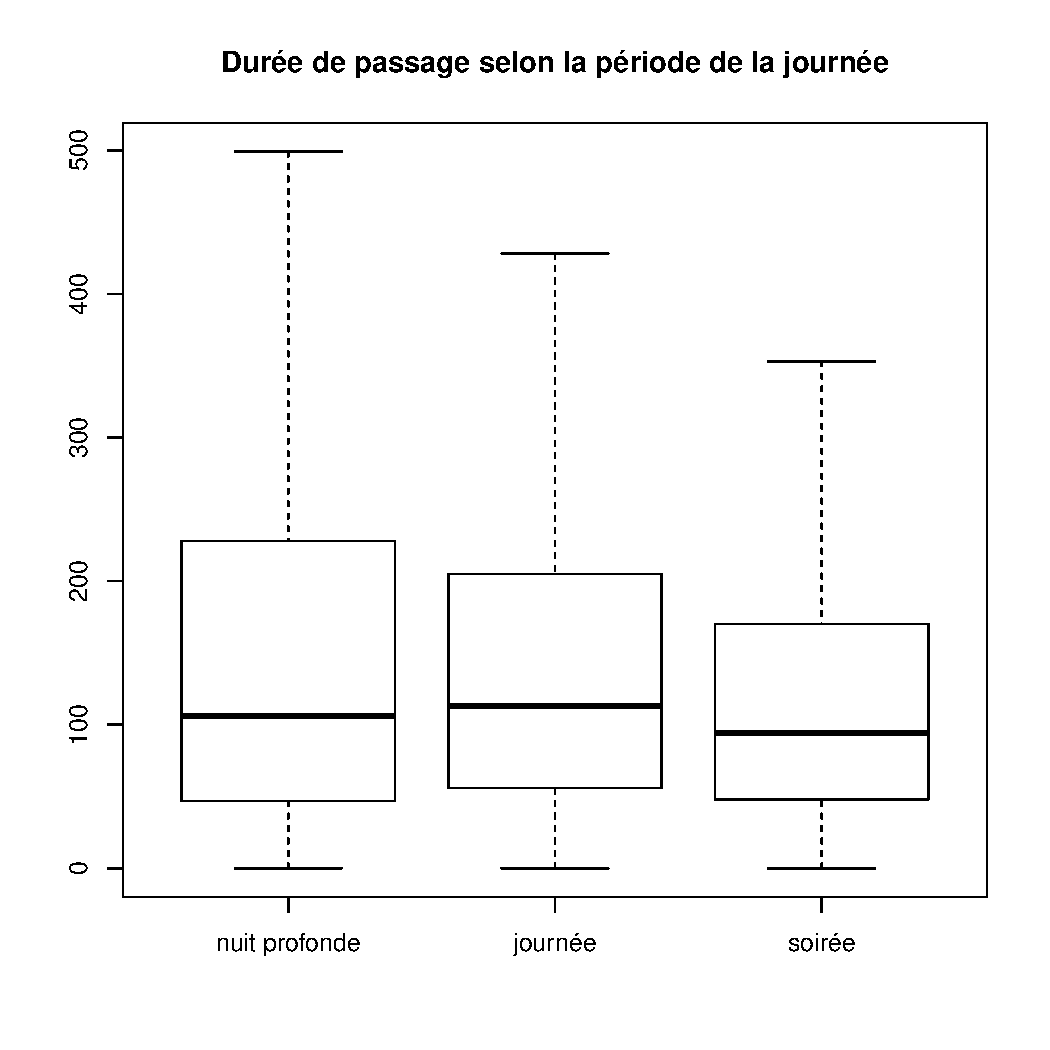
\includegraphics[width=\maxwidth]{figure/duree_heure2} 
\begin{kframe}\begin{verbatim}
## nuit profonde       journée        soirée 
##         183.2         160.9         159.8
\end{verbatim}
\end{kframe}
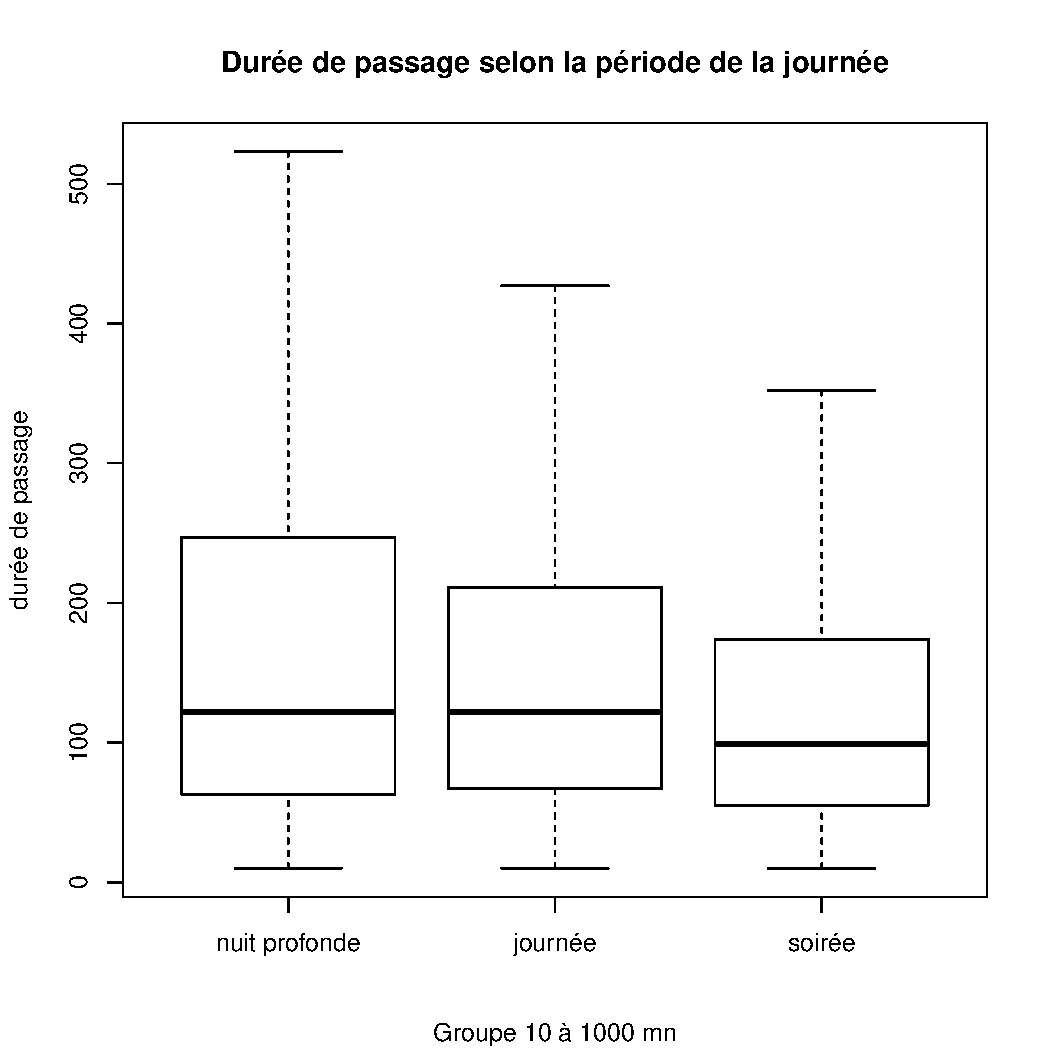
\includegraphics[width=\maxwidth]{figure/duree_heure3} 

\end{knitrout}


\section*{Selon l'âge}

Le temps de passage augmente avec l'age.
\begin{knitrout}
\definecolor{shadecolor}{rgb}{0.969, 0.969, 0.969}\color{fgcolor}\begin{kframe}
\begin{verbatim}
## 15 ans et moins     16 à 74 ans  75 ans et plus 
##            4711           11399            2392
## 15 ans et moins     16 à 74 ans  75 ans et plus 
##           118.5           163.0           244.8
\end{verbatim}
\end{kframe}
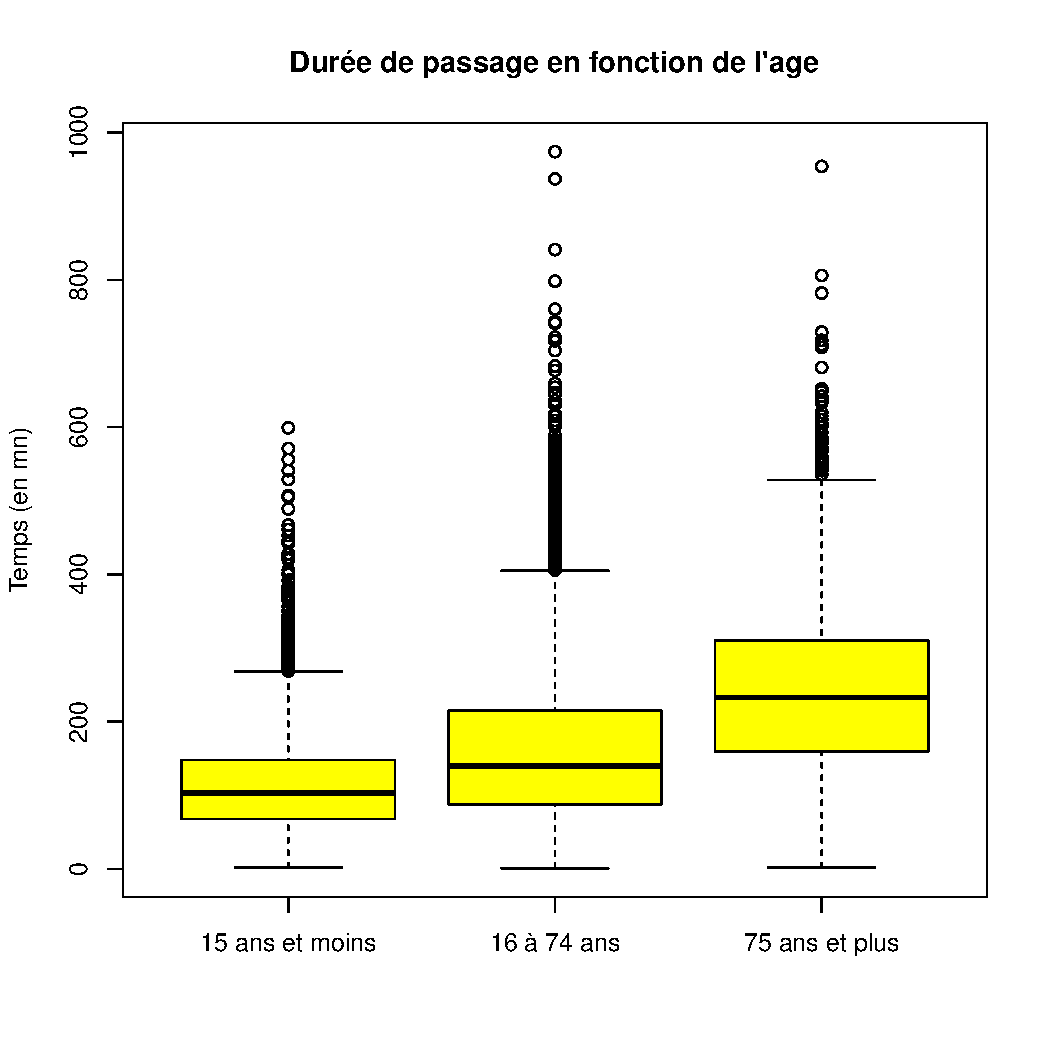
\includegraphics[width=\maxwidth]{figure/duree_age1} 
\begin{kframe}\begin{verbatim}
## 15 ans et moins     16 à 74 ans  75 ans et plus            NA's 
##           65621          191925           44211              10
## 15 ans et moins     16 à 74 ans  75 ans et plus 
##           113.3           169.1           220.3
\end{verbatim}
\end{kframe}
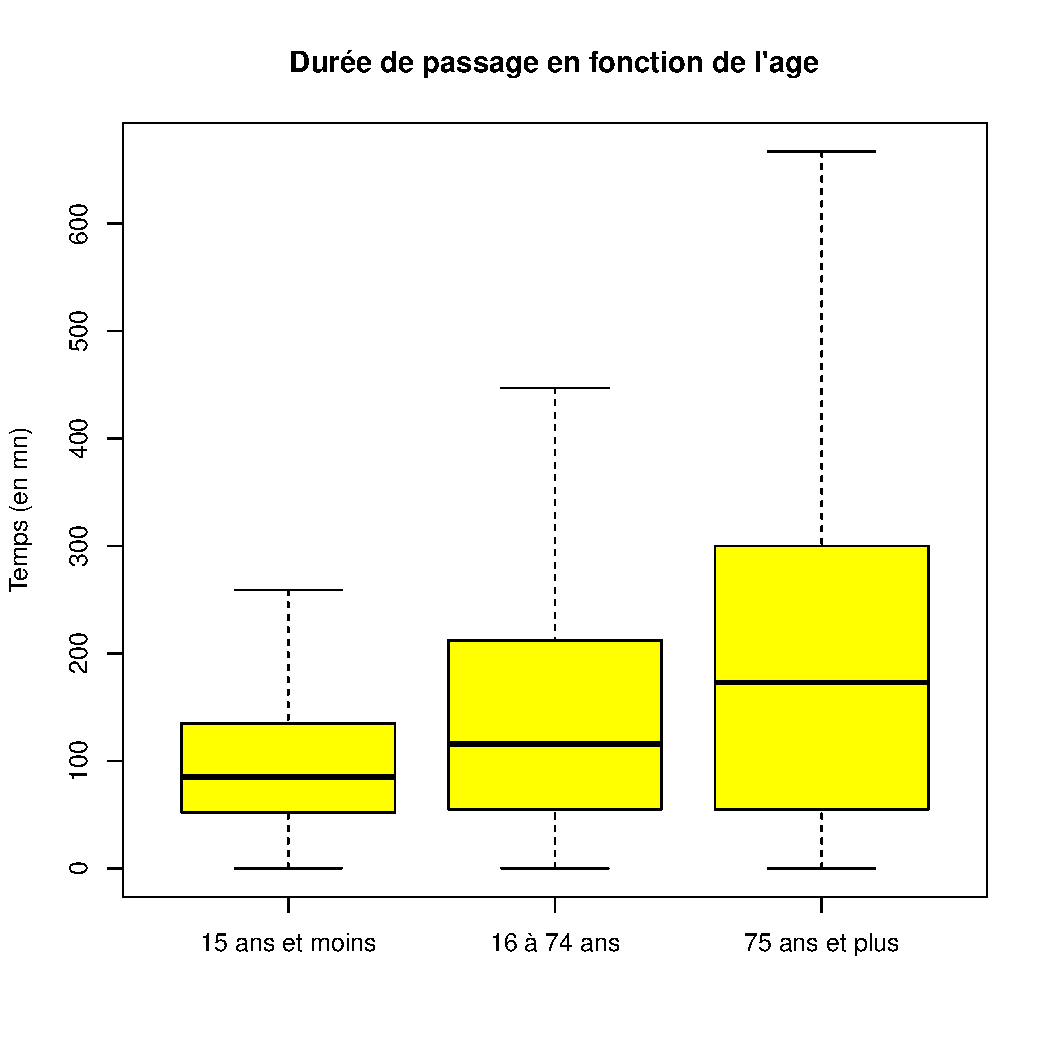
\includegraphics[width=\maxwidth]{figure/duree_age2} 

\end{knitrout}


\section*{Selon le jour de la semaine}
\begin{knitrout}
\definecolor{shadecolor}{rgb}{0.969, 0.969, 0.969}\color{fgcolor}\begin{kframe}
\begin{alltt}
\hlkwd{tapply}\hlstd{(sel}\hlopt{$}\hlstd{p,} \hlkwd{wday}\hlstd{(e,} \hlkwc{label} \hlstd{=} \hlnum{TRUE}\hlstd{), mean,} \hlkwc{na.rm} \hlstd{=} \hlnum{TRUE}\hlstd{)}
\end{alltt}
\begin{verbatim}
##   Sun   Mon  Tues   Wed Thurs   Fri   Sat 
## 142.9 174.8 167.4 159.9 165.3 158.5 165.3
\end{verbatim}
\begin{alltt}
\hlcom{# selon le jour et la période}
\hlstd{t} \hlkwb{<-} \hlkwd{table}\hlstd{(periode,} \hlkwd{wday}\hlstd{(e,} \hlkwc{label} \hlstd{=} \hlnum{TRUE}\hlstd{))}
\end{alltt}


{\ttfamily\noindent\bfseries\color{errorcolor}{\#\# Error: all arguments must have the same length}}\begin{alltt}
\hlstd{t}
\end{alltt}
\begin{verbatim}
## [1] 274140
\end{verbatim}
\begin{alltt}
\hlcom{# tout le groupe}
\hlkwd{tapply}\hlstd{(d1}\hlopt{$}\hlstd{presence,} \hlkwd{wday}\hlstd{(e,} \hlkwc{label} \hlstd{=} \hlnum{TRUE}\hlstd{), mean,} \hlkwc{na.rm} \hlstd{=} \hlnum{TRUE}\hlstd{)}
\end{alltt}


{\ttfamily\noindent\bfseries\color{errorcolor}{\#\# Error: arguments must have same length}}\begin{alltt}
\hlkwd{boxplot}\hlstd{(d1}\hlopt{$}\hlstd{presence} \hlopt{~} \hlkwd{wday}\hlstd{(e,} \hlkwc{label} \hlstd{=} \hlnum{TRUE}\hlstd{),} \hlkwc{outline} \hlstd{= F,} \hlkwc{ylab} \hlstd{=} \hlstr{"durée de présence moyenne (mn)"}\hlstd{,}
    \hlkwc{main} \hlstd{=} \hlstr{"Durée de présence moyenne selon le jour de la semaine"}\hlstd{)}
\end{alltt}


{\ttfamily\noindent\bfseries\color{errorcolor}{\#\# Error: variable lengths differ (found for 'wday(e, label = TRUE)')}}\end{kframe}
\end{knitrout}


\subsection*{Pourcentage de passages en moins de 4 heures par établissement}




A Sélestat, 80.33\% des patients quittent les urgences en moins de quatre heures.

Pour l'ensemble des patients d'Alsace, 80.41\% quittent les urgences en moins de quatre heures.


\section*{Selon l'orientation}
\begin{knitrout}
\definecolor{shadecolor}{rgb}{0.969, 0.969, 0.969}\color{fgcolor}\begin{kframe}
\begin{verbatim}
##  CHIR FUGUE   HDT    HO   MED  OBST   PSA   REA   REO    SC  SCAM    SI 
## 186.9 114.5    NA    NA 226.4 164.1 177.3 196.9    NA 280.0 158.3 193.2 
##  UHCD 
## 197.8
##   DOM   MCO   SLD 
## 147.3 215.1 208.5
##   CHIR  FUGUE    HDT     HO    MED   OBST    PSA    REA    REO     SC 
## 244.30 230.51 224.23 244.68 266.30 234.69 172.79 209.31  86.14 166.03 
##   SCAM     SI   UHCD 
## 269.20 254.31  89.58
##   DOM   HAD   HMS   MCO   PSY   SLD   SSR 
## 156.8 131.8 506.6 182.5 323.6 238.1 325.4
\end{verbatim}
\end{kframe}
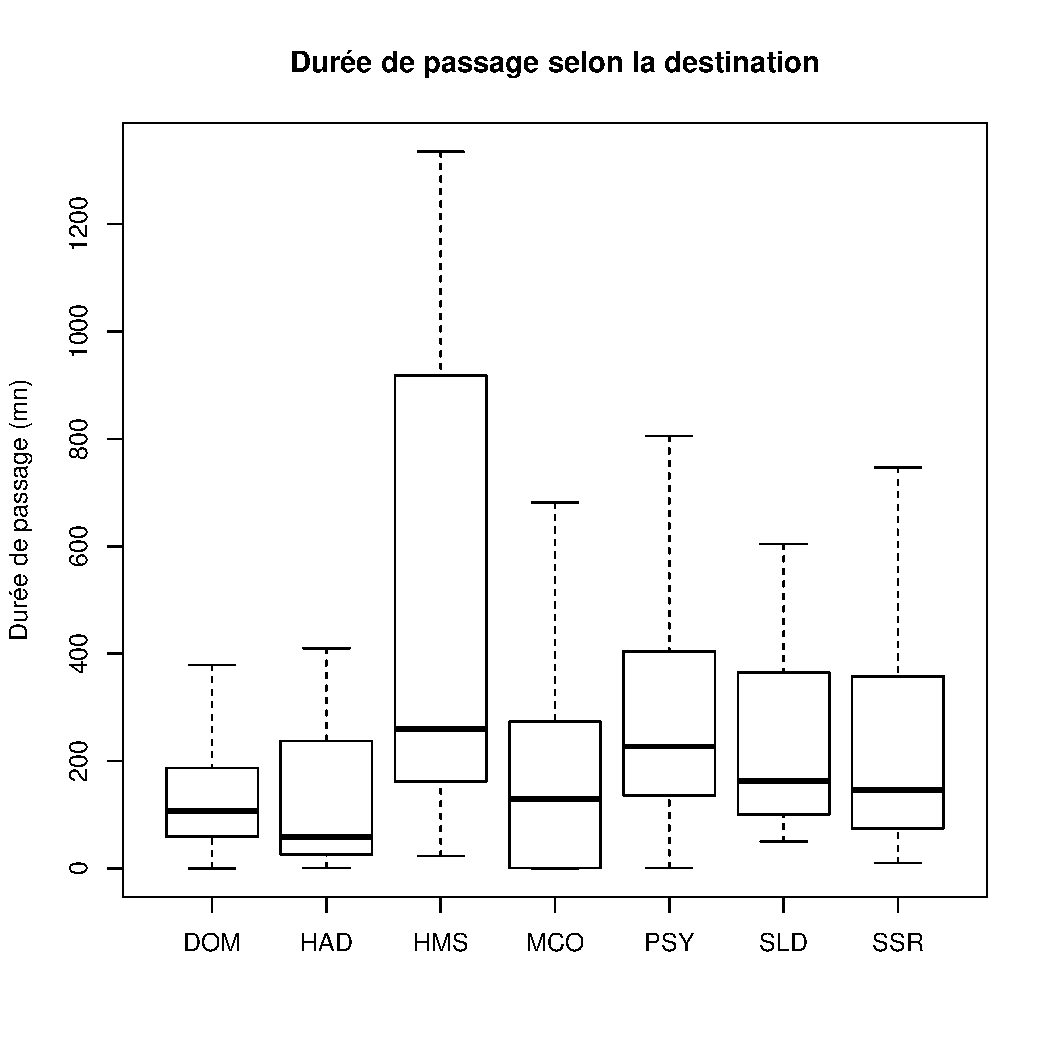
\includegraphics[width=\maxwidth]{figure/duree_orientation} 

\end{knitrout}



\section*{Selon la gravité}
\begin{knitrout}
\definecolor{shadecolor}{rgb}{0.969, 0.969, 0.969}\color{fgcolor}\begin{kframe}
\begin{verbatim}
##     1     2     3     4     5     D     P 
## 106.1 152.1 220.4 213.8 220.0  42.5 151.1
##     1     2     3     4     5     D     P 
## 120.5 159.8 229.0 219.3 176.1 196.8 223.7
\end{verbatim}
\end{kframe}
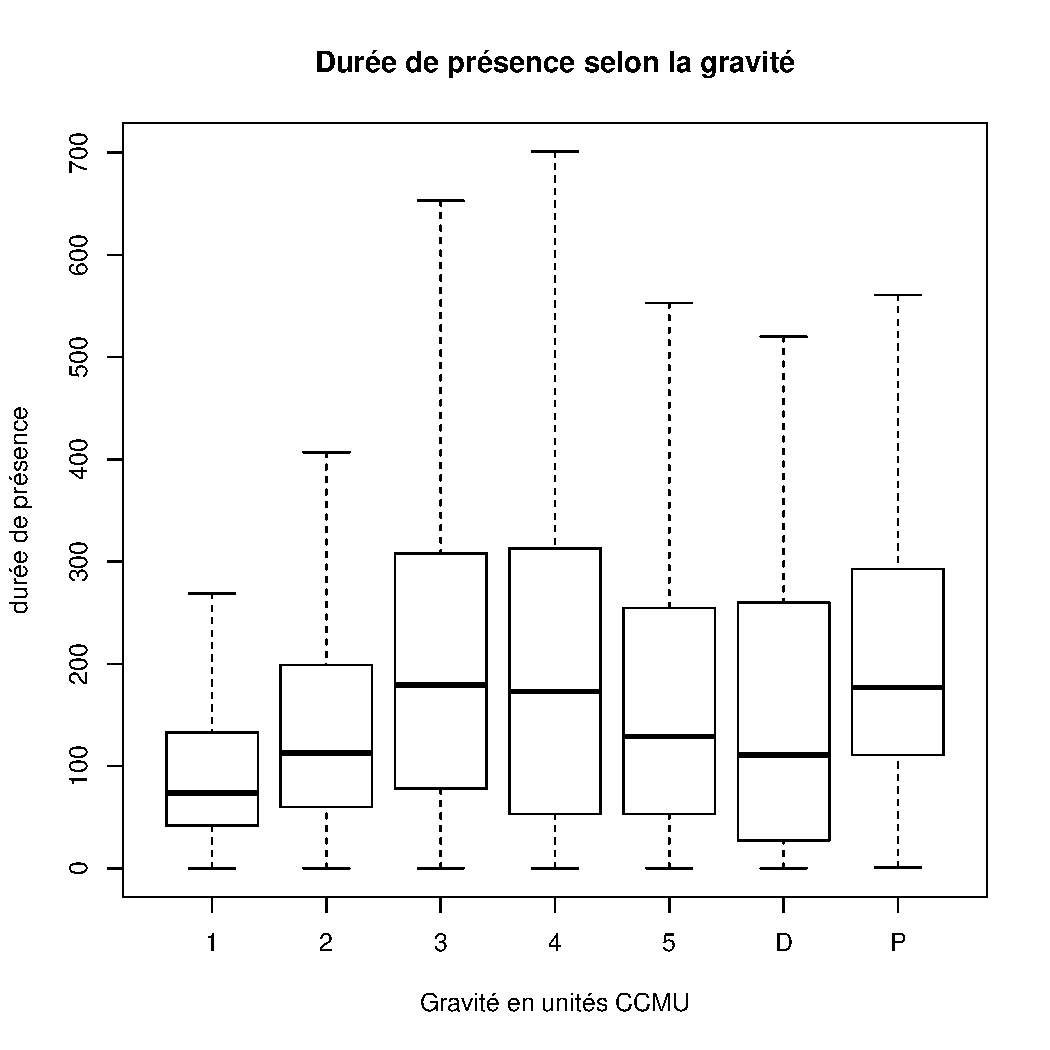
\includegraphics[width=\maxwidth]{figure/duree_gravite} 

\end{knitrout}


\section*{Selon la structure}
\subsection{CH Sélestat}
\begin{knitrout}
\definecolor{shadecolor}{rgb}{0.969, 0.969, 0.969}\color{fgcolor}\begin{kframe}
\begin{verbatim}
##    Min. 1st Qu.  Median    Mean 3rd Qu.    Max.    NA's 
##       1      86     137     162     216     974     627
\end{verbatim}
\end{kframe}
\end{knitrout}



\newpage
\chapter{Codage diagnostique}

%




Les motifs de recours aux urgences sont exprimés en fonction de la classification CIM10 \cite{10}.
\index{motif de recours}
\footnote{Classification Internationale des Maladies, 10ème révision (La CIM10 comporte environ 36000 maladies).}.
\url{http://apps.who.int/classifications/icd10/browse/2008/fr}
Le fichier comporte \np{198659} diagnostics principaux différents.
répartis en 4609 classes de diagnostics.
La comparaison entre le nombre de RPU reçus et le nombre de diagnostics renseignés permet d'établir l'exhaustivité des CIM10 à 65.83\% \index{exhaustivité!CIM10}


\section{Cim10}

Ventilation des diagnostics principaux en fonction des 22 chapitres de la CIM10. Le tableau qui suit indique pour chaque chapitre, le nombre total de cas rapportés, le pourcentage par rapport à l'ensemble, et le pourcentage de cas déduction faite de la traumatologie. En effet celleci représente environ la moitié des cas et il parait intéressant de séparer les pathologies traumatiques des non traumatiques.





%round(prop.table(tr)*100,digits=2)

\begin{longtable}{|c|c|m{4cm}|c|c|c|}
 \hline
 Chapitre & Bloc & Titre & N & \% total  & \% non trauma \\
 \hline
 
I & A00–B99 & Certaines maladies infectieuses et parasitaires & 9384 & 4.72 & 11.05 \\
 II&C00–D48&Tumeurs&938&0.47&1.11\\
 
III&D50–D89&Maladies du sang et des organes hématopoïétiques et certains troubles du système immunitaire&437&0.22&0.51\\

IV&E00–E90&Maladies endocriniennes, nutritionnelles et métaboliques&2237&1.13&2.64\\

V&F00–F99&Troubles mentaux et du comportement&10773&5.42&12.69\\

VI&G00–G99&Maladies du système nerveux&5972&3.01&7.04\\

VII & H00–H59 & Maladies de l'oeil et de ses annexes & 6287 & 3.16&7.41\\

VIII&H60–H95&Maladies de l'oreille et de l'apophyse mastoïde&4437&2.23&5.23\\

IX&I00–I99&Maladies de l'appareil circulatoire&12171&6.13&14.34\\

X&J00–J99&Maladies de l'appareil respiratoire&21341&10.74&25.14\\

XI&K00–K93&Maladies de l'appareil digestif&16016&8.06&18.87\\

XII&L00–L99&Maladies de la peau et du tissu cellulaire souscutané&6060&3.05&7.14\\

XIII&M00–M99&Maladies du système ostéoarticulaire, des muscles et du tissu conjonctif&18320&9.22&21.58\\

XIV&N00–N99&Maladies de l'appareil génitourinaire&10269&5.17&12.1\\

XV&O00–O99&Grossesse, accouchement et puerpéralité&331&0.17&0.39\\

XVI&P00–P96&Certaines affections dont l'origine se situe dans la période périnatale&353&0.18&0.42\\

% XVII&Q00–Q99&Malformations congénitales et anomalies chromosomiques&cong&round(cong*100/total,digits=2)&round(cong*100/(total-traumato),digits=2)\\

XVIII&R00–R99&Symptômes, signes et résultats anormaux d'examens cliniques et de laboratoire, non classés ailleurs&46771&23.54&55.1\\

XIX&S00–T98&Lésions traumatiques, empoisonnements et certaines autres conséquences de causes externes&113774&57.27& \\

XX&V01–Y98&Causes externes de morbidité et de mortalité& 5535&2.79&6.52\\

XXI&Z00–Z99&Facteurs influant sur l'état de santé et motifs de recours aux services de santé&8832&4.45&4.45\\

XXII&U00–U99&Codes d'utilisation particulière & 0&0&0\\

  \hline
\end{longtable}



\begin{knitrout}
\definecolor{shadecolor}{rgb}{0.969, 0.969, 0.969}\color{fgcolor}
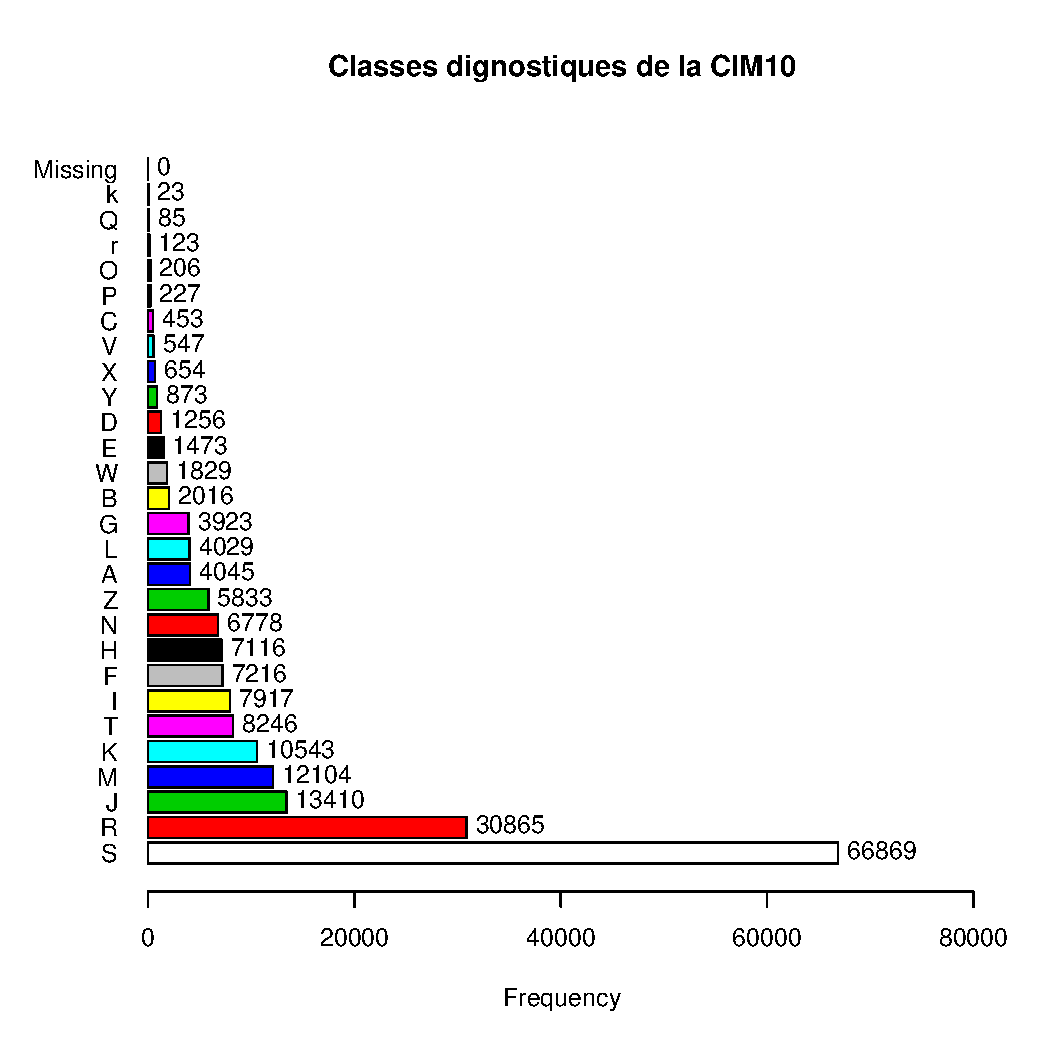
\includegraphics[width=\maxwidth]{figure/class_cim10} 
\begin{kframe}\begin{verbatim}
## a :  
##         Frequency Percent Cum. percent
## S           66869    33.7         33.7
## R           30865    15.5         49.2
## J           13410     6.8         55.9
## M           12104     6.1         62.0
## K           10543     5.3         67.3
## T            8246     4.2         71.5
## I            7917     4.0         75.5
## F            7216     3.6         79.1
## H            7116     3.6         82.7
## N            6778     3.4         86.1
## Z            5833     2.9         89.0
## A            4045     2.0         91.1
## L            4029     2.0         93.1
## G            3923     2.0         95.1
## B            2016     1.0         96.1
## W            1829     0.9         97.0
## E            1473     0.7         97.8
## D            1256     0.6         98.4
## Y             873     0.4         98.8
## X             654     0.3         99.2
## V             547     0.3         99.4
## C             453     0.2         99.7
## P             227     0.1         99.8
## O             206     0.1         99.9
## r             123     0.1         99.9
## Q              85     0.0        100.0
## k              23     0.0        100.0
##   Total    198659   100.0        100.0
\end{verbatim}
\end{kframe}
\end{knitrout}


%%%%%%%%%%%%%%%%%%%%%%%%%%%%%%%%%%%%%%
\section{Etude des AVC}
\index{AVC}
%%%%%%%%%%%%%%%%%%%%%%%%%%%%%%%%%%%%%

Les AVC sont définis par la nomenclature I60 à I64, G45 Accidents ischémiques cérébraux transitoires (sauf G45.4 amnésie transitoire) et syndromes apparentés et G46 Syndromes vasculaires cérébraux au cours de maladies cérébrovasculaires

La prévention et la prise en charge des accidents vasculaires cérébraux  Annexes 
juin 2009

Annexe : Liste exhaustive des codes CIM10 d’AVC

\begin{longtable}{|l|l|}
 \hline
 Code & libellé\\
 \hline
 G450 & Syndrome vertébrobasilaire \\
 G451 & Syndrome carotidien (hémisphérique) \\
 G452 & Accident ischémique transitoire de territoires artériels précérébraux multiples et bilatéraux \\
 G453 & Amaurose fugace \\
 G454 & Amnésie globale transitoire : NON RETENU \\
 G458 & Autres accidents ischémiques cérébraux transitoires et syndromes apparentés \\
 G459 & Accident ischémique cérébral transitoire, sans précision \\
 I600 & Hémorragie sousarachnoïdienne de labifurcation et du siphon carotidien \\
 I601 & Hémorragie sousarachnoïdienne de l'artère cérébrale moyenne \\
 I602 & Hémorragie sousarachnoïdienne de l'artère communicante antérieure \\
 I603 & Hémorragie sousarachnoïdienne del'artère communicante postérieure \\
 I604 & Hémorragie sousarachnoïdienne de l'artère basilaire \\
 I605 & Hémorragie sousarachnoïdienne de l'artère vertébrale \\
 I606 & Hémorragie sousarachnoïdienne d'autres artères intracrâniennes \\
 I607 & Hémorragie sousarachnoïdienne d'une artère intracrânienne, sans précision \\
 I608 & Autres hémorragies sousarachnoïdiennes \\
 I609 & Hémorragie sousarachnoïdienne, sans précision \\
 I610 & Hémorragie intracérébrale hémisphérique, souscorticale \\
 I611 & Hémorragie intracérébrale hémisphérique, corticale \\
 I612 & Hémorragie intracérébrale hémisphérique, non précisée \\
 I613 & Hémorragie intracérébrale du tronc cérébral \\
 I614 & Hémorragie intracérébrale cérébelleuse \\
 I615 & Hémorragie intracérébrale intraventriculaire \\
 I616 & Hémorragie intracérébrale,localisations multiples \\
 I618 & Autres hémorragies intracérébrales \\
 I619 & Hémorragie intracérébrale, sans précision \\
 I620 & Hémorragie sousdurale (aiguë) (non traumatique) \\
 I621 & Hémorragie extradurale non traumatique \\
 I629 & Hémorragie intracrânienne (non traumatique), sans précision \\
 I630 & Infarctus cérébral dû à une thrombose des artères précérébrales \\
 I631 & Infarctus cérébral dû à une embolie des artères précérébrales \\
 I632 & Infarctus cérébral dû à une occlusion ou sténose des artères précérébrales,de mécanisme non précisé \\
 I633 & Infarctus cérébral dû à une thrombose des artères cérébrales \\
 I634 & Infarctus cérébral dû à une embolie des artères cérébrales \\
 I635 & Infarctus cérébral dû à une occlusion ou sténose des artères cérébrales, demécanisme non précisé \\
 I636 & Infarctus cérébral dû à une thrombose veineuse cérébrale, non pyogène \\
 I638 & Autres infarctus cérébraux \\
 I639 & Infarctus cérébral, sans précision \\
 I64 & Accident vasculaire cérébral, non précisé comme étant hémorragique ou par infarctus \\
 G460 & Syndrome de l'artère cérébrale moyenne (I66.0) (1) \\
 G461 & Syndrome de l'artère cérébrale antérieure (I66.1) (1) \\
 G462 & Syndrome de l'artère cérébrale postérieure (I66.2) (1) \\
 G463 & Syndromes vasculaires du tronc cérébral (I60I67) (1) \\
 G464 & Syndrome cérébelleux vasculaire (I60I67) (1) \\
 G465 & Syndrome lacunaire moteur pur (I60I67) (1) \\
 G466 & Syndrome lacunaire sensitif pur (I60I67) (1) \\
 G467 & Autres syndromes lacunaires (I60I67) (1) \\
 G468 & Autres syndromes vasculaires cérébraux au cours de maladies cérébrovasculaires (I60I67) (1) \\
  \hline
\end{longtable}

\begin{knitrout}
\definecolor{shadecolor}{rgb}{0.969, 0.969, 0.969}\color{fgcolor}\begin{kframe}
\begin{alltt}
\hlcom{# Création d'un dataframe DP}
\hlstd{dpr} \hlkwb{<-} \hlstd{d1[}\hlopt{!}\hlkwd{is.na}\hlstd{(d1}\hlopt{$}\hlstd{DP),} \hlkwd{c}\hlstd{(}\hlstr{"DP"}\hlstd{,} \hlstr{"CODE_POSTAL"}\hlstd{,} \hlstr{"ENTREE"}\hlstd{,} \hlstr{"FINESS"}\hlstd{,} \hlstr{"GRAVITE"}\hlstd{,}
    \hlstr{"ORIENTATION"}\hlstd{,} \hlstr{"MODE_SORTIE"}\hlstd{,} \hlstr{"AGE"}\hlstd{,} \hlstr{"SEXE"}\hlstd{,} \hlstr{"TRANSPORT"}\hlstd{)]}
\hlcom{# correction d'erreurs:}
\hlstd{dpr}\hlopt{$}\hlstd{DP[}\hlnum{37807}\hlstd{]} \hlkwb{<-} \hlstr{"N10"}
\hlstd{dpr}\hlopt{$}\hlstd{DP[}\hlnum{47689}\hlstd{]} \hlkwb{<-} \hlstr{"R06.0"}
\hlstd{dpr}\hlopt{$}\hlstd{DP[}\hlnum{68023}\hlstd{]} \hlkwb{<-} \hlstr{"C61"}
\hlstd{dpr}\hlopt{$}\hlstd{DP[}\hlnum{73924}\hlstd{]} \hlkwb{<-} \hlstr{"N10"}
\hlcom{# un peu de ménage:}
\hlstd{dpr}\hlopt{$}\hlstd{DP} \hlkwb{<-} \hlkwd{gsub}\hlstd{(}\hlstr{"."}\hlstd{,} \hlstr{""}\hlstd{,} \hlkwd{as.character}\hlstd{(dpr}\hlopt{$}\hlstd{DP),} \hlkwc{fixed} \hlstd{=} \hlnum{TRUE}\hlstd{)}
\hlstd{dpr}\hlopt{$}\hlstd{DP} \hlkwb{<-} \hlkwd{gsub}\hlstd{(}\hlstr{"+"}\hlstd{,} \hlstr{""}\hlstd{,} \hlkwd{as.character}\hlstd{(dpr}\hlopt{$}\hlstd{DP),} \hlkwc{fixed} \hlstd{=} \hlnum{TRUE}\hlstd{)}
\hlcom{# extraction d'un DF avc:}
\hlstd{AVC} \hlkwb{<-} \hlstd{dpr[}\hlkwd{substr}\hlstd{(dpr}\hlopt{$}\hlstd{DP,} \hlnum{1}\hlstd{,} \hlnum{3}\hlstd{)} \hlopt{>=} \hlstr{"I60"} \hlopt{&} \hlkwd{substr}\hlstd{(dpr}\hlopt{$}\hlstd{DP,} \hlnum{1}\hlstd{,} \hlnum{3}\hlstd{)} \hlopt{<} \hlstr{"I65"} \hlopt{|} \hlkwd{substr}\hlstd{(dpr}\hlopt{$}\hlstd{DP,}
    \hlnum{1}\hlstd{,} \hlnum{3}\hlstd{)} \hlopt{==} \hlstr{"G46"} \hlopt{|} \hlkwd{substr}\hlstd{(dpr}\hlopt{$}\hlstd{DP,} \hlnum{1}\hlstd{,} \hlnum{3}\hlstd{)} \hlopt{==} \hlstr{"G45"}\hlstd{, ]}
\end{alltt}
\end{kframe}
\end{knitrout}


\subsection*{Horaire des AVC}
\index{AVC!heure}

Horaire des AVC, à comparer avec:
\begin{itemize}
  \item les crises d'épilepsie
  \item la pression athmosphérique
\end{itemize}

\begin{knitrout}
\definecolor{shadecolor}{rgb}{0.969, 0.969, 0.969}\color{fgcolor}
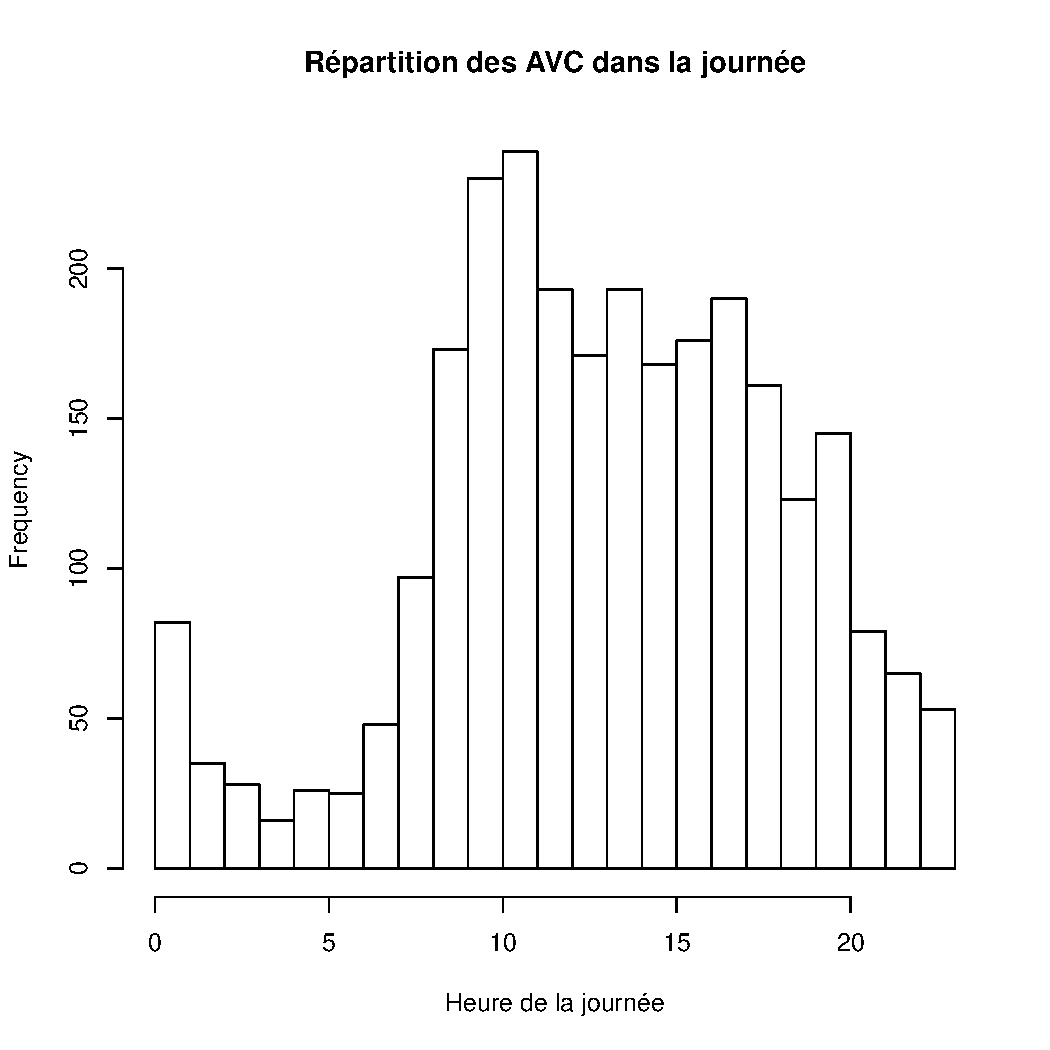
\includegraphics[width=\maxwidth]{figure/heure_avc1} 

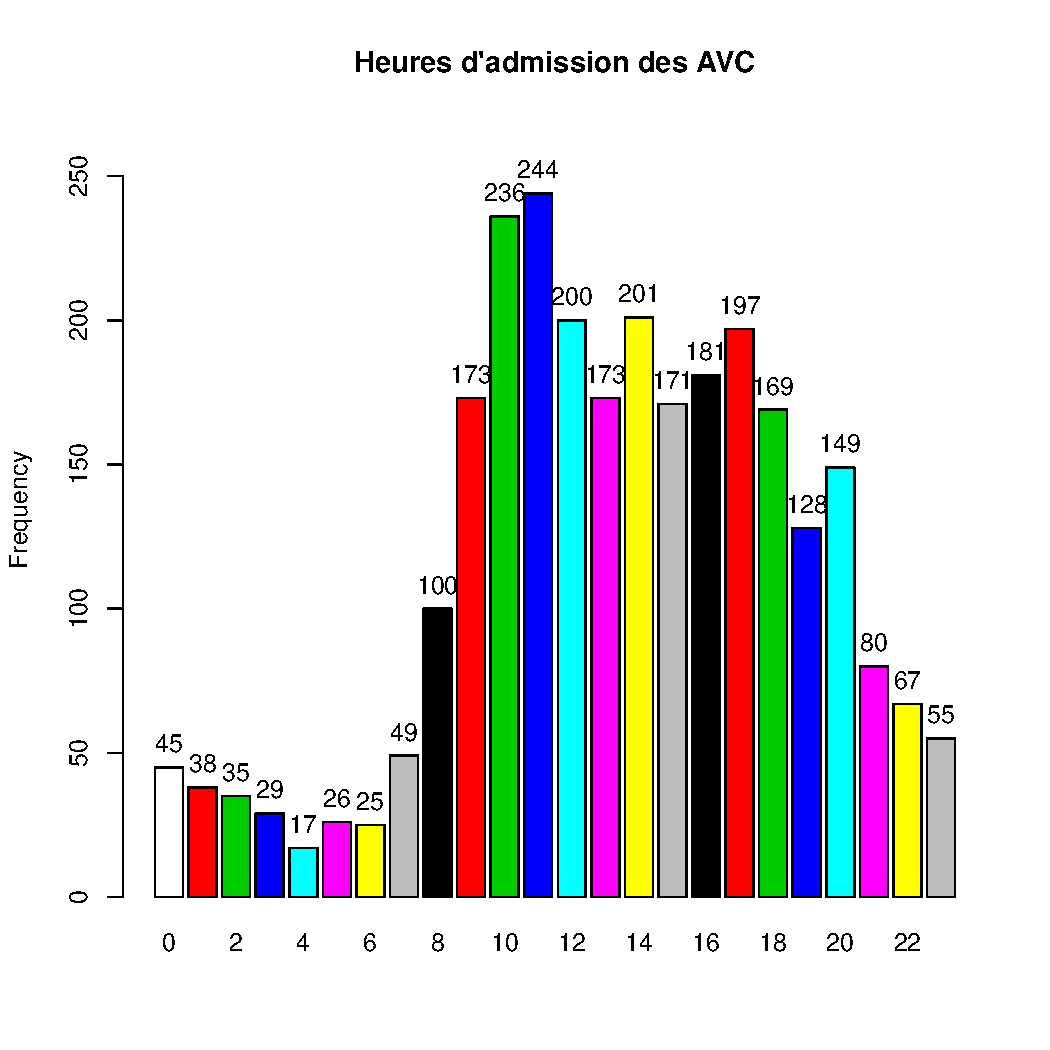
\includegraphics[width=\maxwidth]{figure/heure_avc2} 
\begin{kframe}\begin{verbatim}
## h :  
##         Frequency Percent Cum. percent
## 0              44     1.8          1.8
## 1              34     1.4          3.1
## 2              33     1.3          4.5
## 3              28     1.1          5.6
## 4              16     0.6          6.2
## 5              24     1.0          7.2
## 6              24     1.0          8.2
## 7              42     1.7          9.8
## 8              90     3.6         13.5
## 9             155     6.2         19.7
## 10            210     8.4         28.1
## 11            212     8.5         36.6
## 12            173     6.9         43.6
## 13            157     6.3         49.9
## 14            178     7.1         57.0
## 15            148     5.9         63.0
## 16            163     6.5         69.5
## 17            175     7.0         76.5
## 18            147     5.9         82.4
## 19            117     4.7         87.1
## 20            138     5.5         92.7
## 21             72     2.9         95.6
## 22             60     2.4         98.0
## 23             50     2.0        100.0
##   Total      2490   100.0        100.0
\end{verbatim}
\end{kframe}
\end{knitrout}


\subsection*{Selon le jour de la semaine}
\index{AVC!age}

\begin{knitrout}
\definecolor{shadecolor}{rgb}{0.969, 0.969, 0.969}\color{fgcolor}\begin{kframe}
\begin{verbatim}
## w
## Dim Lun Mar Mer Jeu Ven Sam 
## 290 397 403 369 362 360 309
## w
##   Dim   Lun   Mar   Mer   Jeu   Ven   Sam 
## 11.65 15.94 16.18 14.82 14.54 14.46 12.41
\end{verbatim}
\end{kframe}
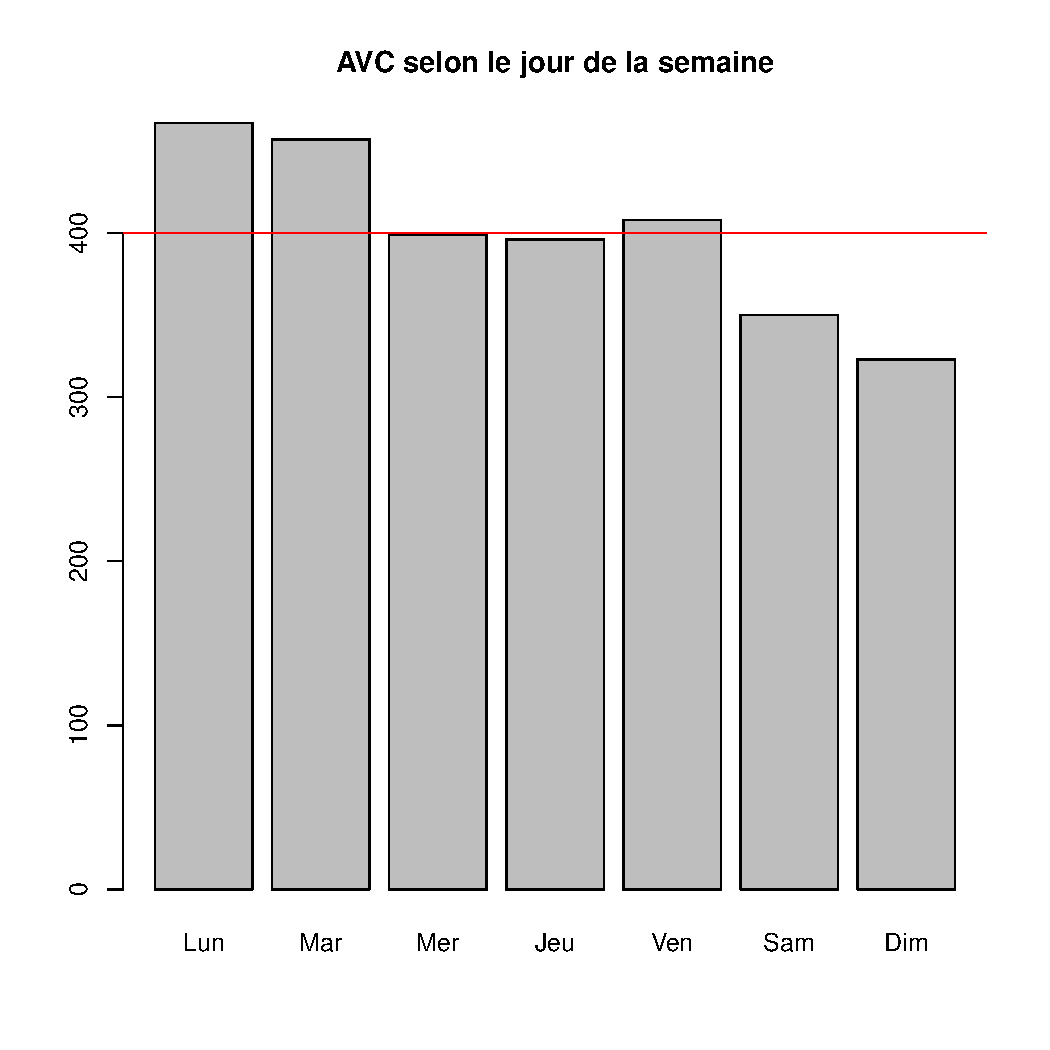
\includegraphics[width=\maxwidth]{figure/avc_jour_semaine} 

\end{knitrout}

Proportion théorique = 14.28\% par jour de la semaine.

\subsection*{AVC et age}
\index{AVC!age}
\begin{knitrout}
\definecolor{shadecolor}{rgb}{0.969, 0.969, 0.969}\color{fgcolor}\begin{kframe}
\begin{verbatim}
##    Min. 1st Qu.  Median    Mean 3rd Qu.    Max. 
##     1.0    61.0    75.0    71.1    83.0   112.0
\end{verbatim}
\end{kframe}
\end{knitrout}

Le rapport de 2009 donne age moyen = 70.5 et age médian = 75 ans.

\subsection*{AVC et sexe}
\index{AVC!sexe}
\begin{knitrout}
\definecolor{shadecolor}{rgb}{0.969, 0.969, 0.969}\color{fgcolor}\begin{kframe}
\begin{verbatim}
##    F    I    M 
## 1299    0 1191
\end{verbatim}
\end{kframe}
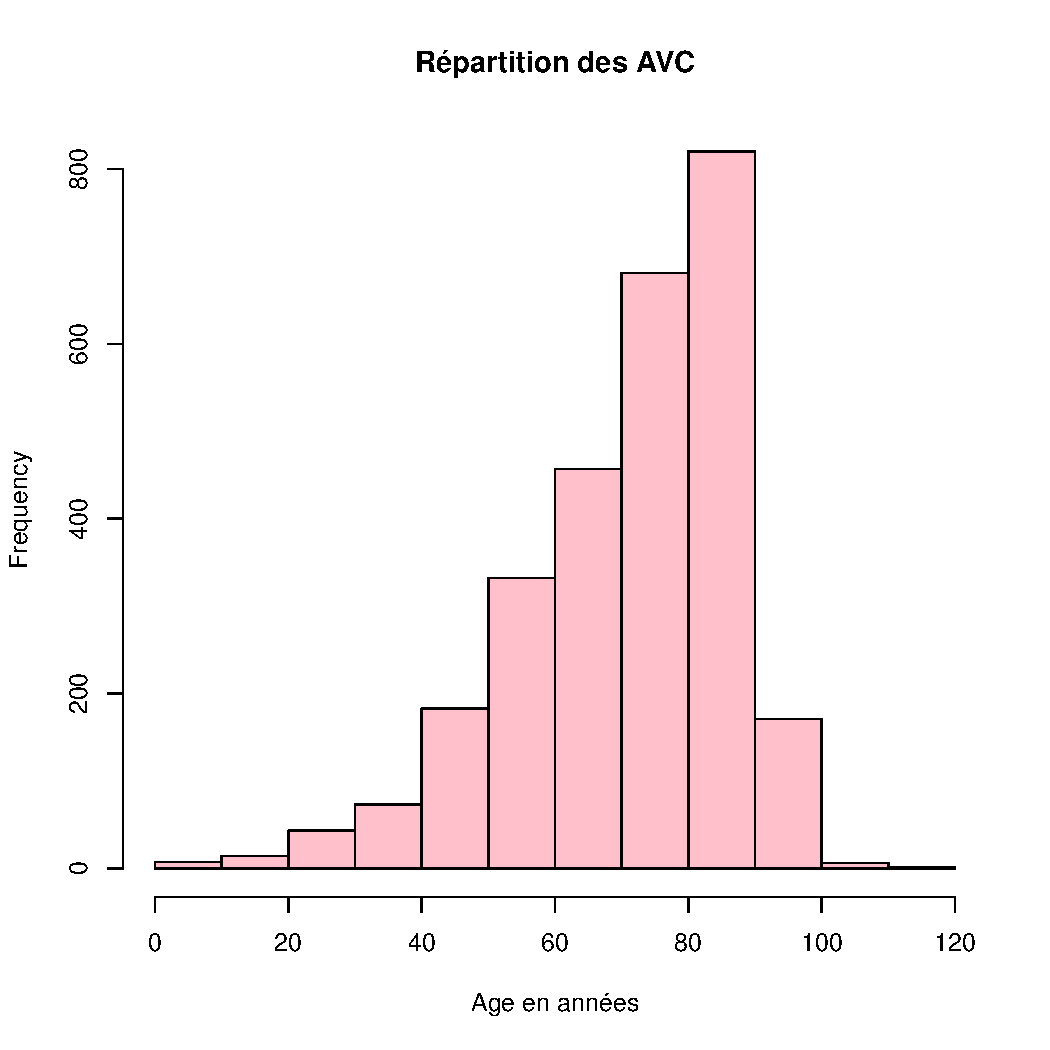
\includegraphics[width=\maxwidth]{figure/avc_sexe1} 

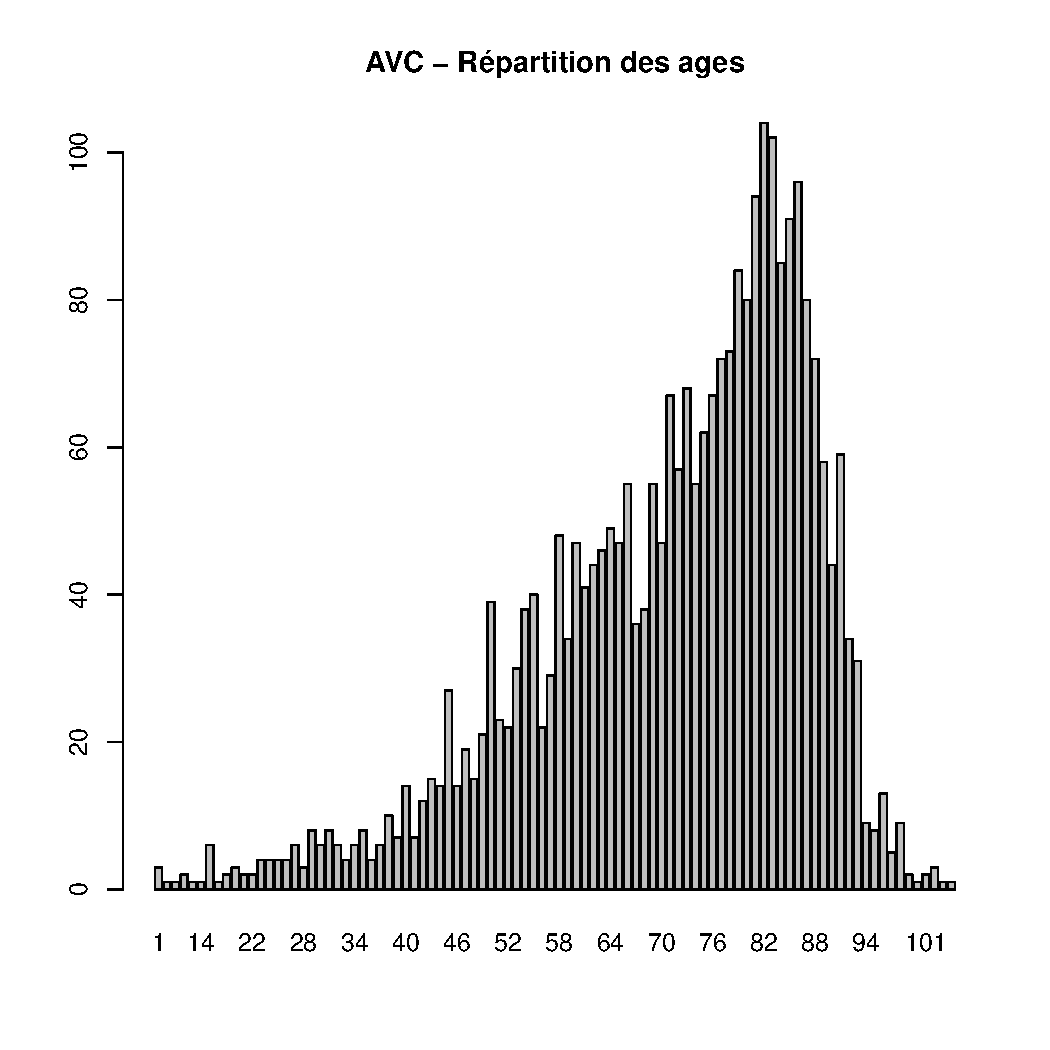
\includegraphics[width=\maxwidth]{figure/avc_sexe2} 

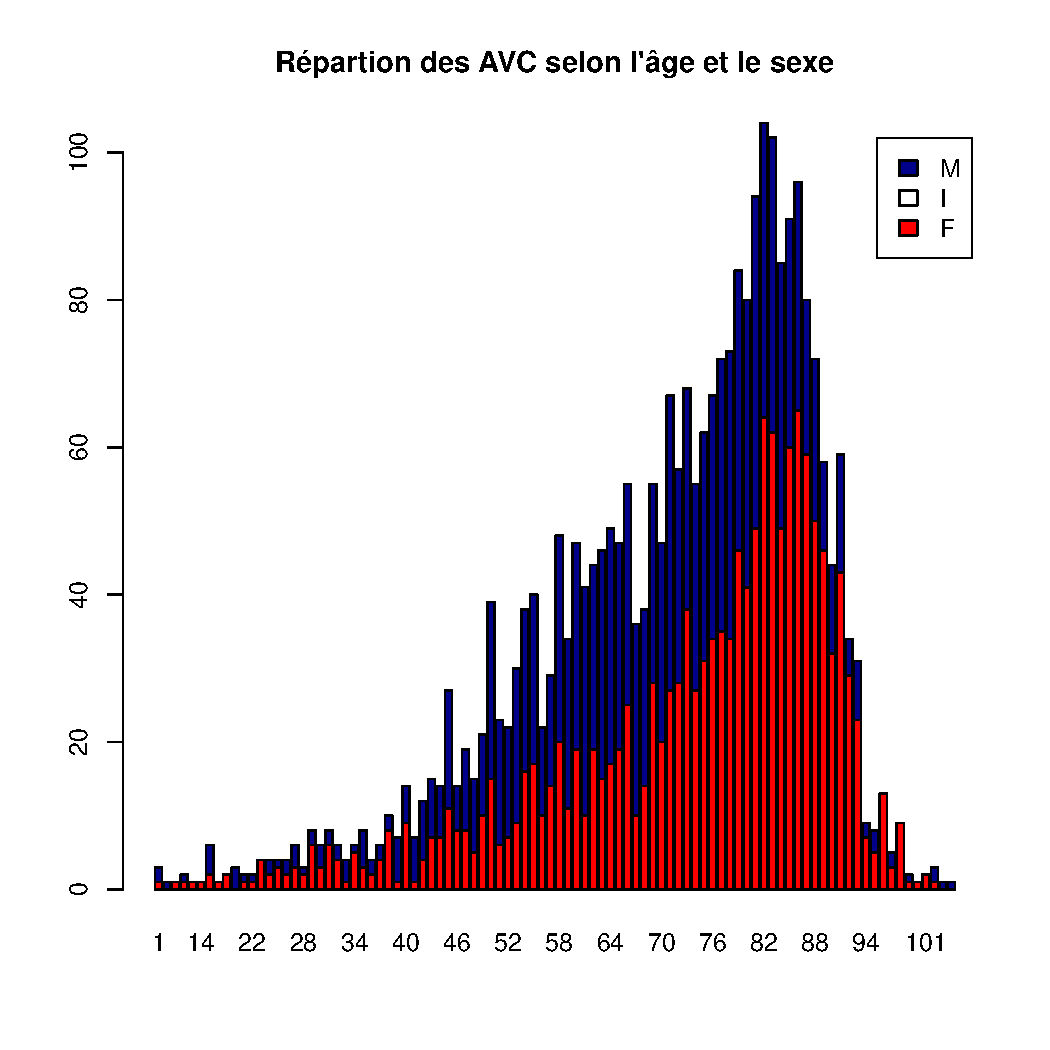
\includegraphics[width=\maxwidth]{figure/avc_sexe3} 

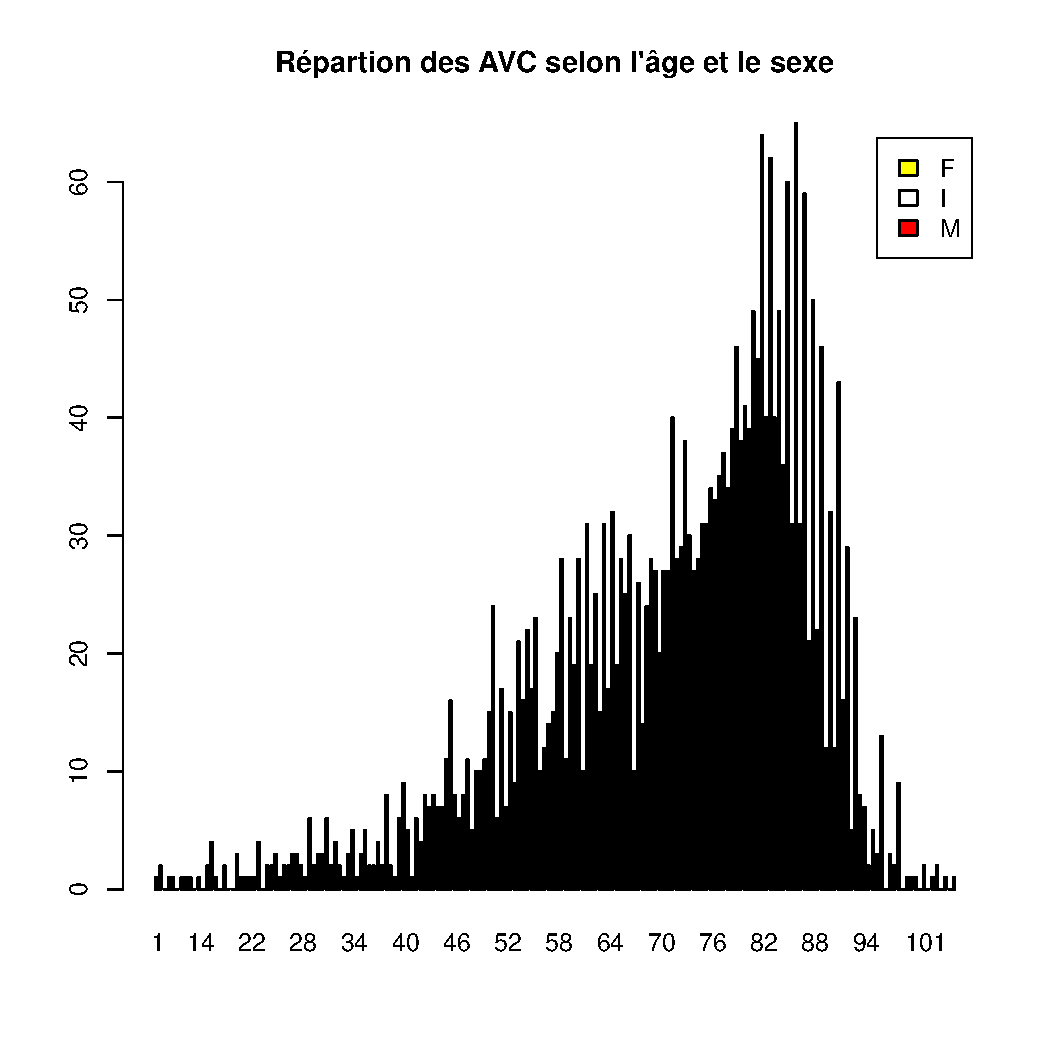
\includegraphics[width=\maxwidth]{figure/avc_sexe4} 

\end{knitrout}


%%%%%%%%%%%%%%%%%%%%%%%%%%%%%%%%%%%%%%%%%%%%%%%%%%%
\section{Accidents ischiémiques transitoires (AIT)}
\index{AIT}
%%%%%%%%%%%%%%%%%%%%%%%%%%%%%%%%%%%%%%%%%%%%%%%%%%%

Recommandations pour la sélection des données PMSI MCO concernant l’AVC (Juin 2009)

\begin{longtable}{|l|l|}
 \hline
 Code & libellé\\
 \hline
G450 & Syndrome vertébro-basilaire \\
G451 & Syndrome carotidien (hémisphérique) \\
G452 & Accident ischémique transitoire de territoires artériels précérébraux multiples et bilatéraux \\
G453  & Amaurose fugace \\
G458  & Autres accidents ischémiques cérébraux transitoires et syndromes apparentés \\
G459  & Accident ischémique cérébral transitoire, sans précision \\  
  \hline
\end{longtable}

Le thésaurus SFMU (2013) \cite{9} recommande d'utiliser G45.9 (ou G459) pour tout diagnostic d'AIT.
\index{AIT!thésaurus}

\begin{knitrout}
\definecolor{shadecolor}{rgb}{0.969, 0.969, 0.969}\color{fgcolor}
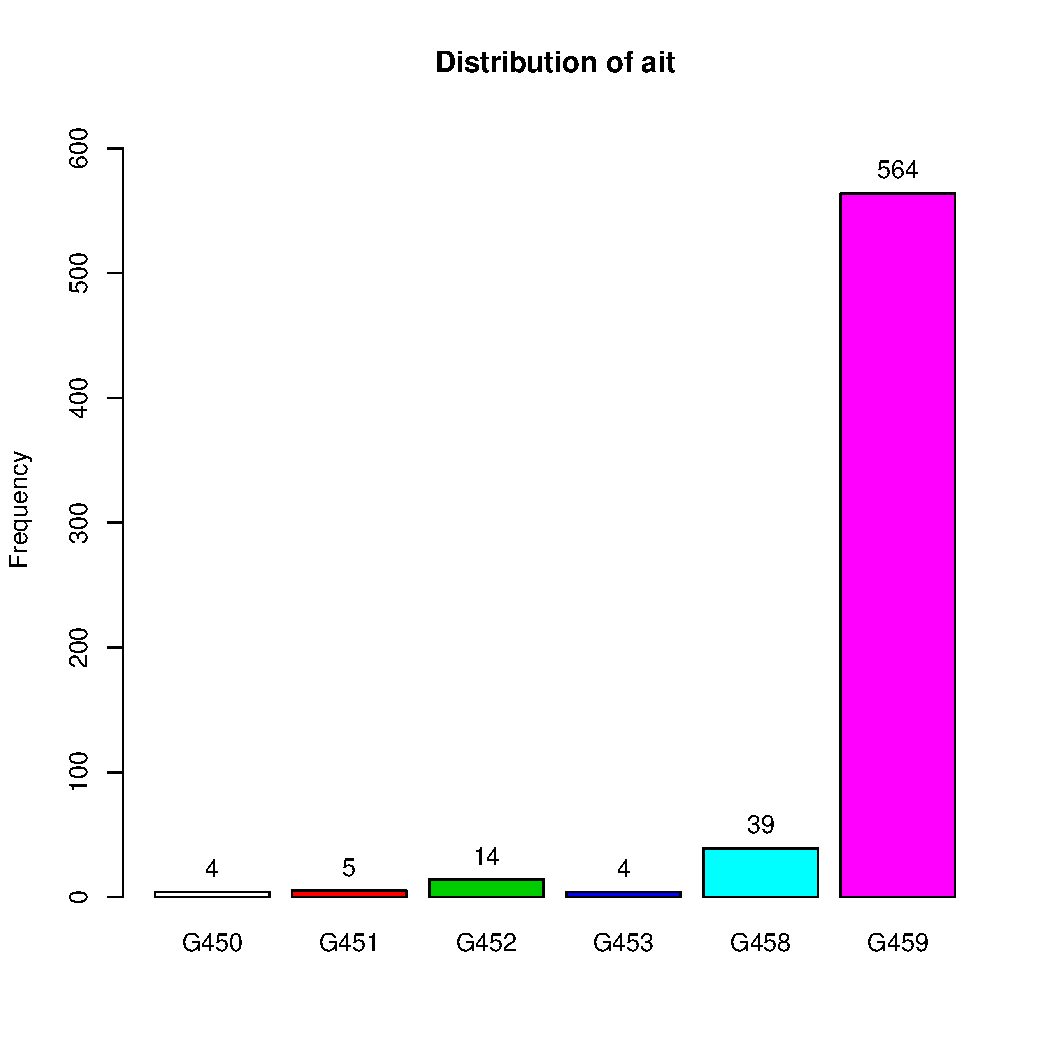
\includegraphics[width=\maxwidth]{figure/ait} 
\begin{kframe}\begin{verbatim}
## ait :  
##         Frequency Percent Cum. percent
## G450            4     0.6          0.6
## G451            5     0.8          1.4
## G452           14     2.2          3.7
## G453            4     0.6          4.3
## G458           39     6.2         10.5
## G459          564    89.5        100.0
##   Total       630   100.0        100.0
\end{verbatim}
\end{kframe}
\end{knitrout}


%%%%%%%%%%%%%%%%%%%%%%%%%%%%%
\section{Pneumonies}
\index{pneumonies}
%%%%%%%%%%%%%%%%%%%%%%%%%%%%

\begin{knitrout}
\definecolor{shadecolor}{rgb}{0.969, 0.969, 0.969}\color{fgcolor}\begin{kframe}


{\ttfamily\noindent\color{warningcolor}{\#\# Warning: impossible d'ouvrir le fichier '../mes\_fonctions.R' : Aucun fichier ou dossier de ce type}}

{\ttfamily\noindent\bfseries\color{errorcolor}{\#\# Error: impossible d'ouvrir la connexion}}\begin{verbatim}
## [1] "Pneumonies et AGE"
##    Min. 1st Qu.  Median    Mean 3rd Qu.    Max. 
##       0      62      77      71      85      98
\end{verbatim}
\end{kframe}
\end{knitrout}


Les pneumopaties bactériennes sans précision sont cotées J15.9 Dans la CIM10.
722 diagnostics de ce type ont été portés au SAU en 2013.

Les pneumonies bactériennes concernent les adultes agés des deux sexes. L'age moyen est de 71 ans et la moitié de ces patients ont 77 ans et plus.

\begin{knitrout}
\definecolor{shadecolor}{rgb}{0.969, 0.969, 0.969}\color{fgcolor}
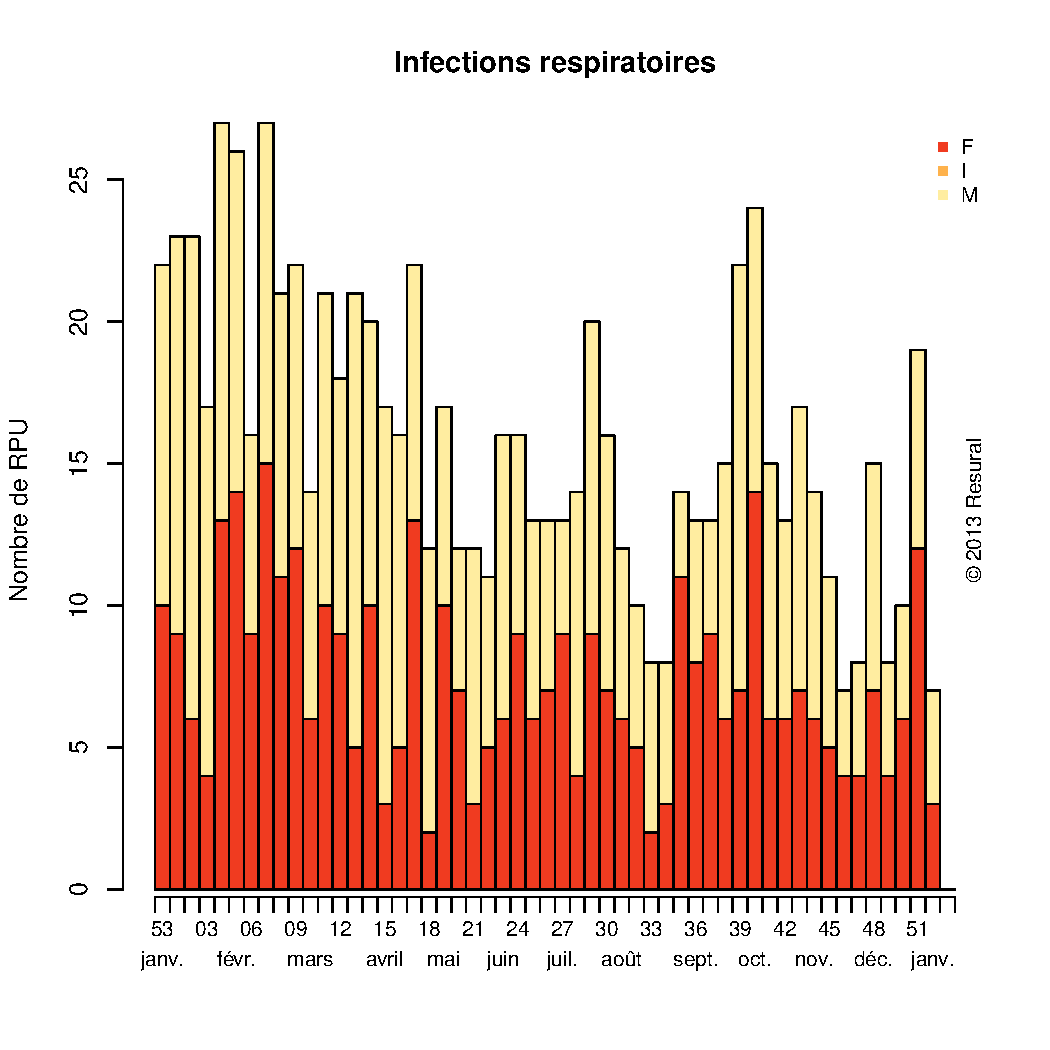
\includegraphics[width=\maxwidth]{figure/pneumo} 

\end{knitrout}


En fonction de la gravité (CCMU):
\begin{knitrout}
\definecolor{shadecolor}{rgb}{0.969, 0.969, 0.969}\color{fgcolor}\begin{kframe}
\begin{verbatim}
##    1    2    3    4    5    D    P NA's 
##   15  319  321   51    6    0    0   10
\end{verbatim}
\end{kframe}
\end{knitrout}


En fonction de la destination:
\begin{knitrout}
\definecolor{shadecolor}{rgb}{0.969, 0.969, 0.969}\color{fgcolor}\begin{kframe}
\begin{verbatim}
## integer(0)
\end{verbatim}
\end{kframe}
\end{knitrout}


En fonction de l'orientation:
\begin{knitrout}
\definecolor{shadecolor}{rgb}{0.969, 0.969, 0.969}\color{fgcolor}\begin{kframe}
\begin{verbatim}
##  CHIR FUGUE   HDT    HO   MED  OBST   PSA   REA   REO    SC  SCAM    SI 
##    10     0     0     0   220     0     0     9     0     5     0     2 
##  UHCD  NA's 
##   227   249
\end{verbatim}
\end{kframe}
\end{knitrout}


Deux patients porteurs de problèmes respiratoires sont orienté en chirurgie : erreur ou manque de place en médecine ?

%%%%%%%%%%%%%%%%%%%%%%%%%%%
\section{Syndrome grippal}
\index{syndrome grippal}
%%%%%%%%%%%%%%%%%%%%%%%%%%%

\begin{knitrout}
\definecolor{shadecolor}{rgb}{0.969, 0.969, 0.969}\color{fgcolor}
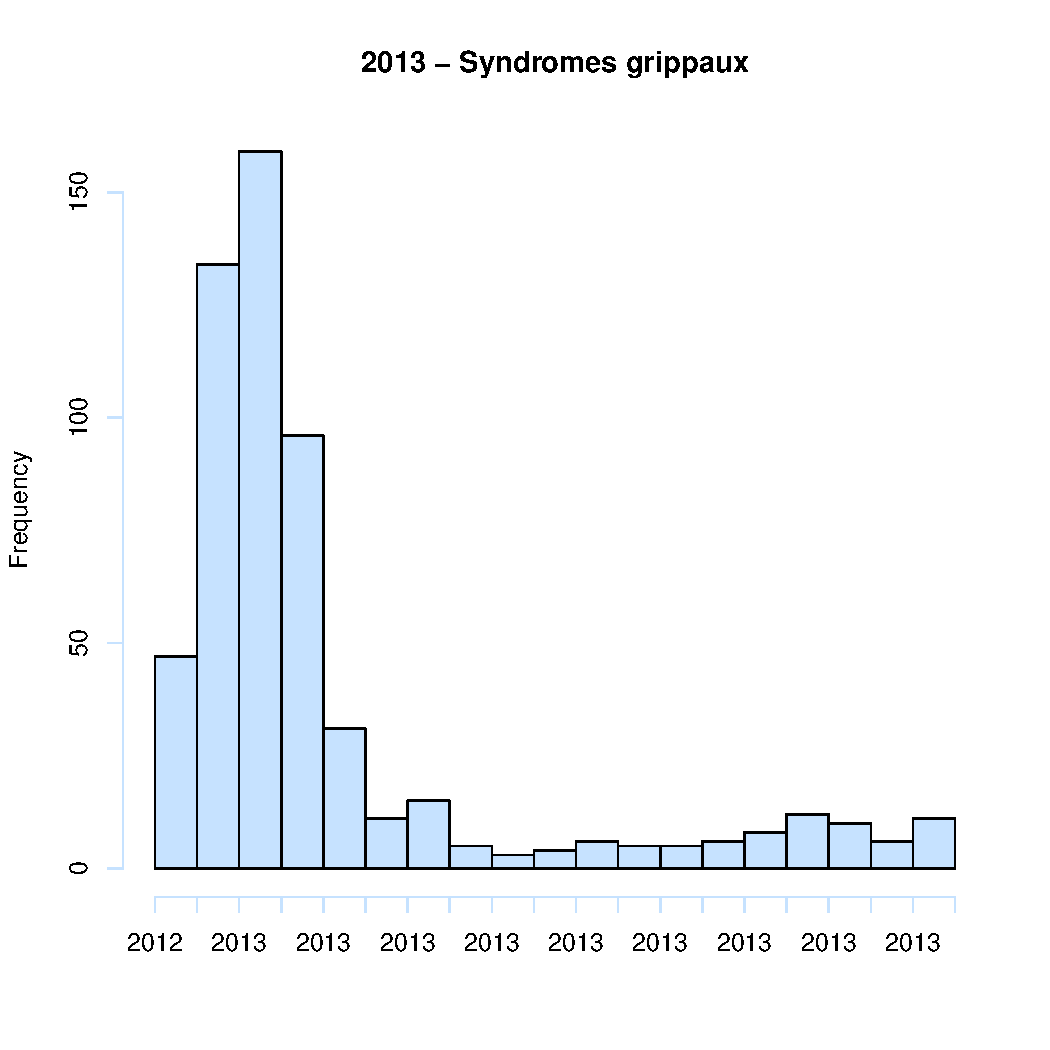
\includegraphics[width=\maxwidth]{figure/grippe} 

\end{knitrout}


%%%%%%%%%%%%%%%%%%%%%%%%%%%%%%%
\section{Asthme}
\index{Asthme}
%%%%%%%%%%%%%%%%%%%%%%%%%%%%%%%

Classification selon la CIM10:
\begin{itemize}
  \item J45.0 Asthme à prédominance allergique
  \item J45.1 Asthme non allergique
  \item J45.8 Asthme associé 
  \item J45.9 Asthme, sans précision
  \item J46   Etat de mal asthmatique
\end{itemize}

% latex table generated in R 3.0.2 by xtable 1.7-1 package
% Sat Dec 21 11:32:39 2013
\begin{table}[ht]
\centering
\begin{tabular}{rr}
  \hline
 & V1 \\ 
  \hline
J450 & 108 \\ 
  J451 & 171 \\ 
  J458 &   5 \\ 
  J459 & 872 \\ 
  J46 &  48 \\ 
   \hline
\end{tabular}
\end{table}

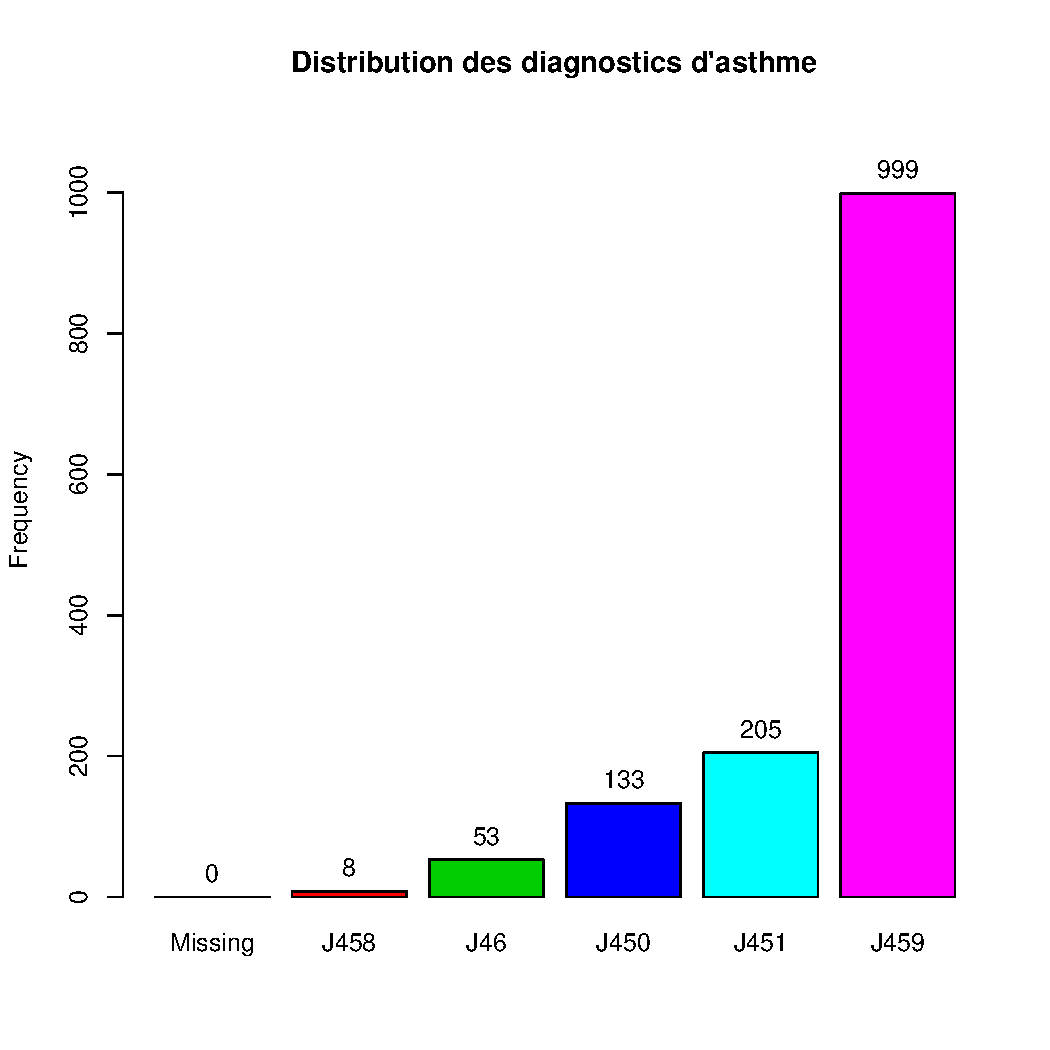
\includegraphics[width=\maxwidth]{figure/asthme} 
% latex table generated in R 3.0.2 by xtable 1.7-1 package
% Sat Dec 21 11:32:39 2013
\begin{table}[ht]
\centering
\begin{tabular}{rrrr}
  \hline
 & Fréquence & Pourcentage & Pourcentage Cumul. \\ 
  \hline
J458 & 5.00 & 0.40 & 0.40 \\ 
  J46 & 48.00 & 4.00 & 4.40 \\ 
  J450 & 108.00 & 9.00 & 13.40 \\ 
  J451 & 171.00 & 14.20 & 27.60 \\ 
  J459 & 872.00 & 72.40 & 100.00 \\ 
    Total & 1204.00 & 100.00 & 100.00 \\ 
   \hline
\end{tabular}
\caption[Répartition des diagnostics d'asthme]{Répartition des diagnostics d'asthme chez les patients ayant consulté un  SU, en région Alsace en 2013} 
\label{tab:asthme}
\end{table}



On note \np{1204} cas d'asthme en 2013.


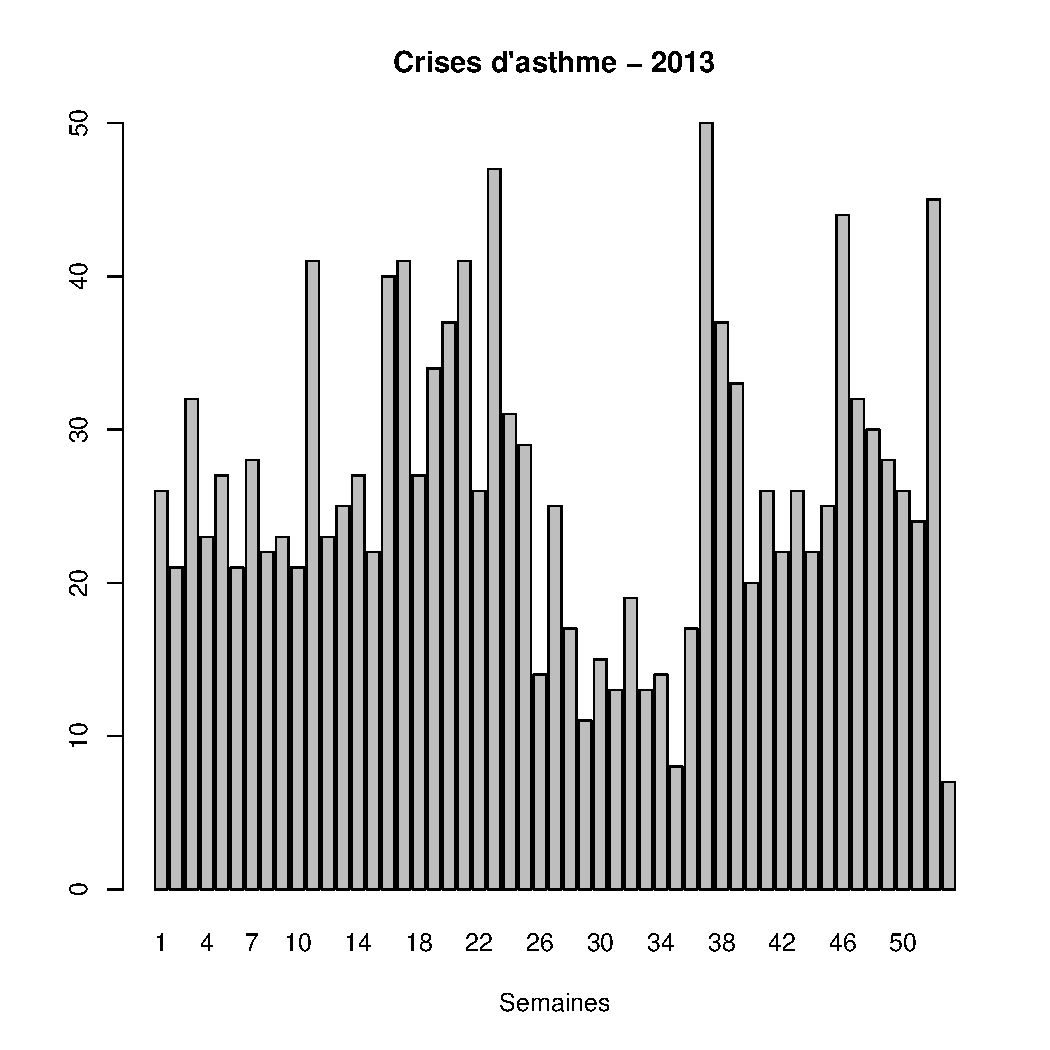
\includegraphics[width=\maxwidth]{figure/asthme21} 

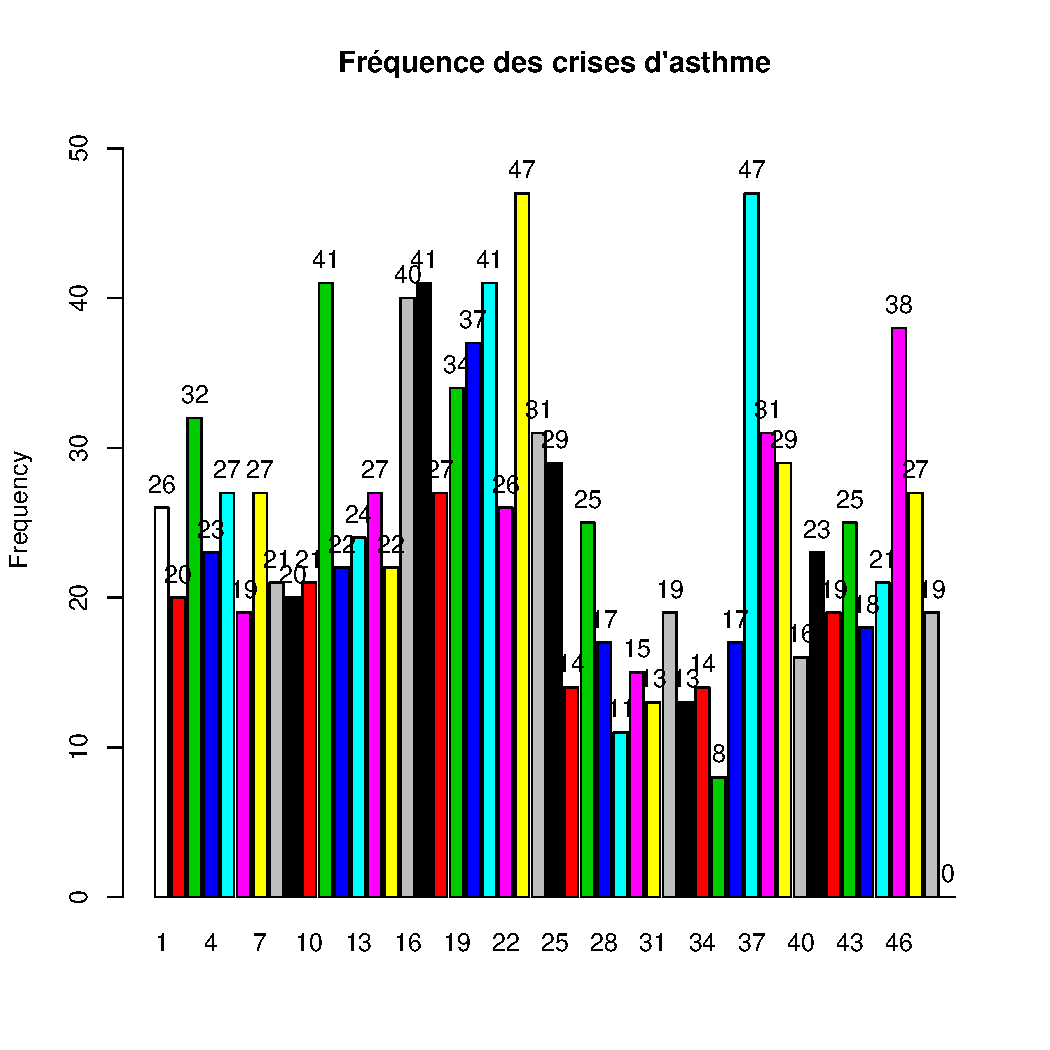
\includegraphics[width=\maxwidth]{figure/asthme22} 
% latex table generated in R 3.0.2 by xtable 1.7-1 package
% Sat Dec 21 11:32:39 2013
\begin{table}[ht]
\centering
\begin{tabular}{rrrr}
  \hline
 & Fréquence & Pourcentage & Pourcentage cumul. \\ 
  \hline
1 & 26.00 & 2.20 & 2.20 \\ 
  2 & 20.00 & 1.70 & 3.80 \\ 
  3 & 32.00 & 2.70 & 6.50 \\ 
  4 & 23.00 & 1.90 & 8.40 \\ 
  5 & 27.00 & 2.20 & 10.60 \\ 
  6 & 19.00 & 1.60 & 12.20 \\ 
  7 & 27.00 & 2.20 & 14.50 \\ 
  8 & 21.00 & 1.70 & 16.20 \\ 
  9 & 20.00 & 1.70 & 17.90 \\ 
  10 & 21.00 & 1.70 & 19.60 \\ 
  11 & 41.00 & 3.40 & 23.00 \\ 
  12 & 22.00 & 1.80 & 24.80 \\ 
  13 & 24.00 & 2.00 & 26.80 \\ 
  14 & 27.00 & 2.20 & 29.10 \\ 
  15 & 22.00 & 1.80 & 30.90 \\ 
  16 & 40.00 & 3.30 & 34.20 \\ 
  17 & 41.00 & 3.40 & 37.60 \\ 
  18 & 27.00 & 2.20 & 39.90 \\ 
  19 & 34.00 & 2.80 & 42.70 \\ 
  20 & 37.00 & 3.10 & 45.80 \\ 
  21 & 41.00 & 3.40 & 49.20 \\ 
  22 & 26.00 & 2.20 & 51.30 \\ 
  23 & 47.00 & 3.90 & 55.20 \\ 
  24 & 31.00 & 2.60 & 57.80 \\ 
  25 & 29.00 & 2.40 & 60.20 \\ 
  26 & 14.00 & 1.20 & 61.40 \\ 
  27 & 25.00 & 2.10 & 63.50 \\ 
  28 & 17.00 & 1.40 & 64.90 \\ 
  29 & 11.00 & 0.90 & 65.80 \\ 
  30 & 15.00 & 1.20 & 67.00 \\ 
  31 & 13.00 & 1.10 & 68.10 \\ 
  32 & 19.00 & 1.60 & 69.70 \\ 
  33 & 13.00 & 1.10 & 70.80 \\ 
  34 & 14.00 & 1.20 & 71.90 \\ 
  35 & 8.00 & 0.70 & 72.60 \\ 
  36 & 17.00 & 1.40 & 74.00 \\ 
  37 & 47.00 & 3.90 & 77.90 \\ 
  38 & 31.00 & 2.60 & 80.50 \\ 
  39 & 29.00 & 2.40 & 82.90 \\ 
  40 & 16.00 & 1.30 & 84.20 \\ 
  41 & 23.00 & 1.90 & 86.10 \\ 
  42 & 19.00 & 1.60 & 87.70 \\ 
  43 & 25.00 & 2.10 & 89.80 \\ 
  44 & 18.00 & 1.50 & 91.30 \\ 
  45 & 21.00 & 1.70 & 93.00 \\ 
  46 & 38.00 & 3.20 & 96.20 \\ 
  47 & 27.00 & 2.20 & 98.40 \\ 
  48 & 19.00 & 1.60 & 100.00 \\ 
    Total & 1204.00 & 100.00 & 100.00 \\ 
   \hline
\end{tabular}
\caption[Fréquence des crises d'asthme]{Fréquence des crises d'asthme par semaine en 2013} 
\label{tab:freq_asthme}
\end{table}




La population des patients consultant pour une crise d'astme est jeune (voir table \ref{tab:age_asthme} page \pageref{tab:age_asthme}).

% latex table generated in R 3.0.2 by xtable 1.7-1 package
% Sat Dec 21 11:32:39 2013
\begin{table}[ht]
\centering
\begin{tabular}{rrrrrrr}
  \hline
 & moyenne & écart-type & médiane & min & max & n \\ 
  \hline
1 & 23.40 & 24.06 & 14.00 & 0.00 & 97.00 & 1204.00 \\ 
   \hline
\end{tabular}
\caption[Asthme et age]{Age de la population consultant pour crise d'asthme} 
\label{tab:age_asthme}
\end{table}
% latex table generated in R 3.0.2 by xtable 1.7-1 package
% Sat Dec 21 11:32:39 2013
\begin{table}[ht]
\centering
\begin{tabular}{rrrrrrrrr}
  \hline
 & 1 & 2 & 3 & 4 & 5 & D & P & NA's \\ 
  \hline
1 & 135 & 749 & 282 &  20 &   4 &   0 &   0 &  14 \\ 
   \hline
\end{tabular}
\caption[Asthme et CCMU]{Gravité de la crise d'asthme en fonction de la CCMU} 
\label{tab:ccmu_asthme}
\end{table}



Les crises sont de gravité moyenne avec une prédominance de CCMU 2 et 3 (voir table \ref{tab:ccmu_asthme} page \pageref{tab:ccmu_asthme}).
Cependant le taux d'hospitalisation est important: 38.72 \%.
\np{79} patients ont été orientés vers un service "chaud" (Réanimation, sins intensifs ou continus) soit 19.41 \% des patients hospitalisés pour asthme.

Le bulletin épidémiologique (Le point épidémiologique du 24 octobre 2013 - Surveillance épidémiologique de la Cire Lorraine-Alsace) clôt la surveillance de l’asthme. Pour l’association SOS Médecins de Strasbourg, l’activité liée à l’asthme a été particulièrement marqué de mi-avril (semaine 16) à fin mai(semaine 22) puis en semaine 40. Concernant l’association de Mulhouse, seule une forte augmentation en semaine 39 a été observée depuis début avril.

%%%%%%%%%%%%%%%%%%%%%%%%%%%%
\section{Bronchiolite}
\index{Bronchiolite}
%%%%%%%%%%%%%%%%%%%%%%%%%%%%

CIM10: Bronchiolite aiguë

Inclus:
    avec bronchospasme
\begin{itemize}
  \item J21.0 Bronchiolite aiguë due au virus respiratoire syncytial [VRS]
  \item J21.8 Bronchiolite aiguë due à d'autres micro-organismes précisés
  \item J21.9 Bronchiolite aiguë, sans précision
\end{itemize}

\begin{knitrout}
\definecolor{shadecolor}{rgb}{0.969, 0.969, 0.969}\color{fgcolor}\begin{kframe}
\begin{alltt}
\hlstd{bron} \hlkwb{<-} \hlstd{dpr[}\hlkwd{substr}\hlstd{(dpr}\hlopt{$}\hlstd{DP,} \hlnum{1}\hlstd{,} \hlnum{3}\hlstd{)} \hlopt{==} \hlstr{"J21"}\hlstd{, ]}
\hlstd{m} \hlkwb{<-} \hlkwd{month}\hlstd{(bron}\hlopt{$}\hlstd{ENTREE,} \hlkwc{label} \hlstd{= T)}
\hlkwd{barplot}\hlstd{(}\hlkwd{table}\hlstd{(m),} \hlkwc{main} \hlstd{=} \hlstr{"Bronchiolites - 2013"}\hlstd{,} \hlkwc{xlab} \hlstd{=} \hlstr{"Mois"}\hlstd{)}
\end{alltt}
\end{kframe}
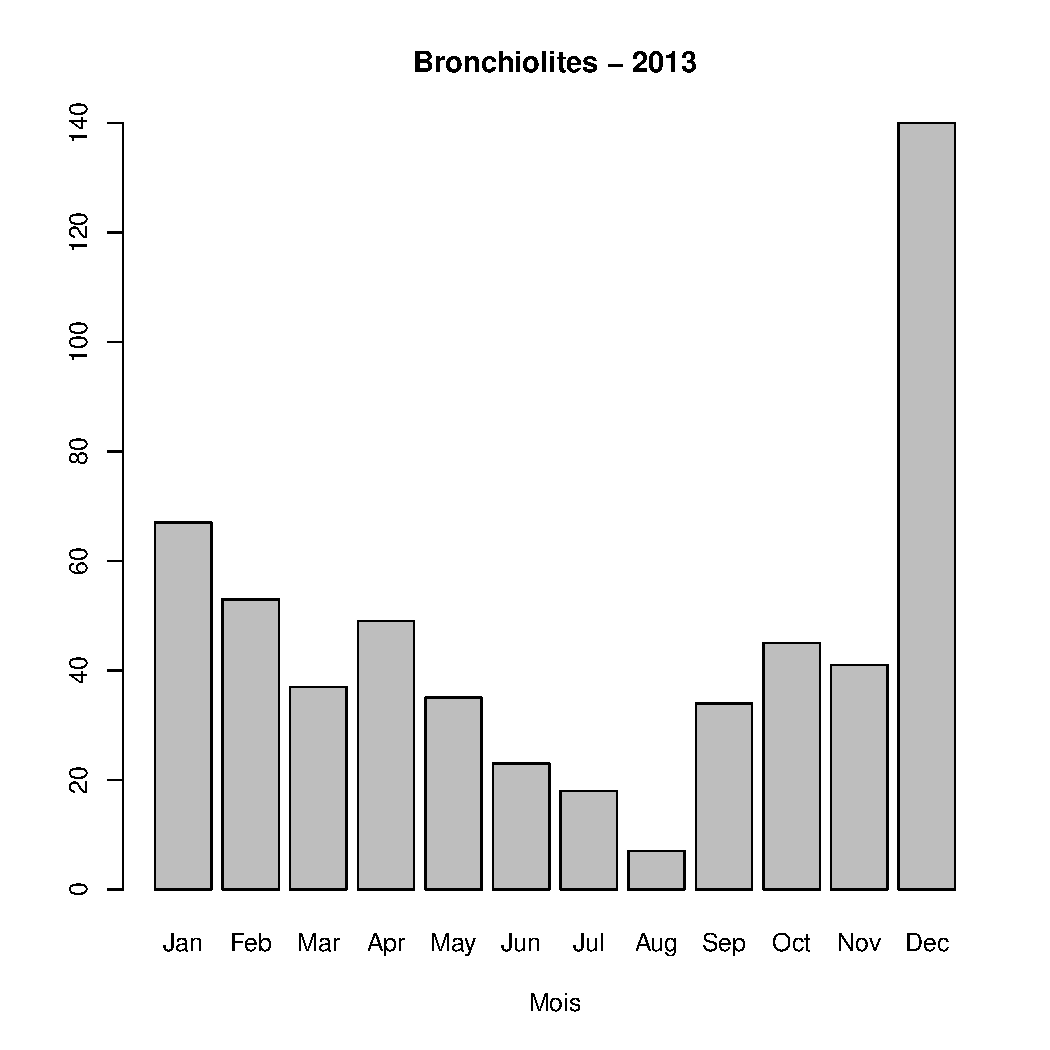
\includegraphics[width=\maxwidth]{figure/bron1} 
\begin{kframe}\begin{alltt}
\hlstd{s} \hlkwb{<-} \hlkwd{week}\hlstd{(bron}\hlopt{$}\hlstd{ENTREE)}
\hlkwd{barplot}\hlstd{(}\hlkwd{table}\hlstd{(s),} \hlkwc{main} \hlstd{=} \hlstr{"Bronchiolites - 2013"}\hlstd{,} \hlkwc{xlab} \hlstd{=} \hlstr{"Semaines"}\hlstd{)}
\end{alltt}
\end{kframe}
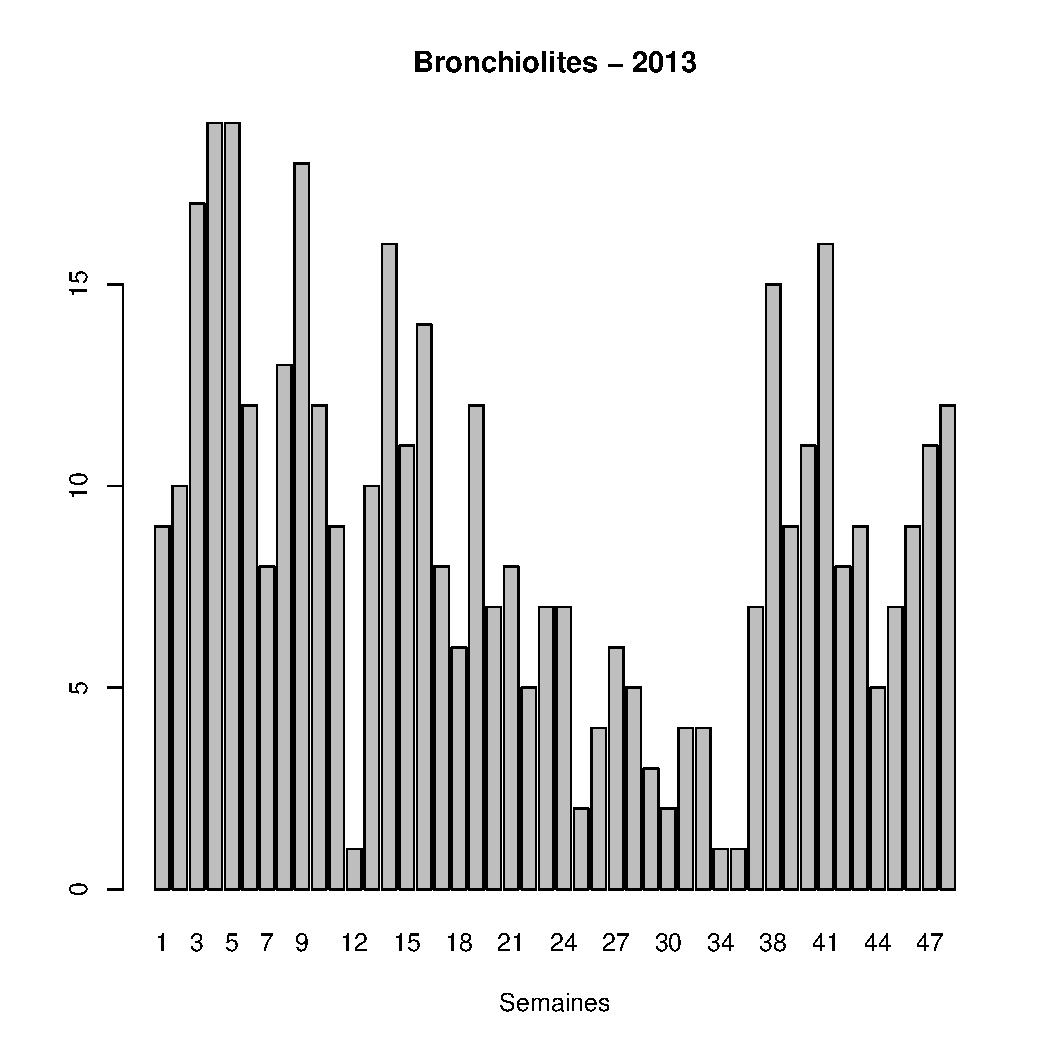
\includegraphics[width=\maxwidth]{figure/bron2} 
\begin{kframe}\begin{alltt}
\hlkwd{summary}\hlstd{(bron)}
\end{alltt}
\begin{verbatim}
##       DP             CODE_POSTAL     ENTREE              FINESS   
##  Length:409         68200  : 81   Length:409         Mul    :334  
##  Class :character   68100  : 59   Class :character   Sel    : 24  
##  Mode  :character   68270  : 21   Mode  :character   Col    : 20  
##                     68300  : 12                      Wis    : 14  
##                     67160  : 10                      3Fr    : 10  
##                     68130  : 10                      Geb    :  2  
##                     (Other):216                      (Other):  5  
##     GRAVITE     ORIENTATION     MODE_SORTIE       AGE        SEXE   
##  2      :220   SC     : 91   NA       :  0   Min.   : 0.00   F:175  
##  3      :132   MED    : 88   Mutation :185   1st Qu.: 0.00   I:  0  
##  1      : 46   REA    :  4   Transfert:  0   Median : 0.00   M:234  
##  4      :  5   UHCD   :  3   Domicile :190   Mean   : 1.15          
##  5      :  3   SCAM   :  1   Décès    :  0   3rd Qu.: 0.00          
##  (Other):  0   (Other):  0   NA's     : 34   Max.   :93.00          
##  NA's   :  3   NA's   :222                                          
##  TRANSPORT  
##  AMBU :  9  
##  FO   :  0  
##  HELI :  0  
##  PERSO:358  
##  SMUR :  0  
##  VSAB :  3  
##  NA's : 39
\end{verbatim}
\end{kframe}
\end{knitrout}


Surreprésentation de Mul  
taux hospitalisation: 50\%


%%%%%%%%%%%%%%%%%%%%%%%%%%%%
\section{Intoxication au CO}
\index{Intoxication au CO}
%%%%%%%%%%%%%%%%%%%%%%%%%%%%

CIM10 = T58

\begin{knitrout}
\definecolor{shadecolor}{rgb}{0.969, 0.969, 0.969}\color{fgcolor}\begin{kframe}
\begin{alltt}
\hlstd{co} \hlkwb{<-} \hlstd{dpr[}\hlkwd{substr}\hlstd{(dpr}\hlopt{$}\hlstd{DP,} \hlnum{1}\hlstd{,} \hlnum{3}\hlstd{)} \hlopt{==} \hlstr{"T58"}\hlstd{, ]}
\hlstd{m} \hlkwb{<-} \hlkwd{month}\hlstd{(co}\hlopt{$}\hlstd{ENTREE,} \hlkwc{label} \hlstd{= T)}
\hlkwd{table}\hlstd{(m)}
\end{alltt}
\begin{verbatim}
## m
## Jan Feb Mar Apr May Jun Jul Aug Sep Oct Nov Dec 
##   5  12  11   0   6   9   0   1   0   1  13   0
\end{verbatim}
\begin{alltt}
\hlkwd{barplot}\hlstd{(}\hlkwd{table}\hlstd{(m),} \hlkwc{main} \hlstd{=} \hlstr{"Intoxication au CO - 2013"}\hlstd{,} \hlkwc{xlab} \hlstd{=} \hlstr{"Mois"}\hlstd{)}
\end{alltt}
\end{kframe}
\includegraphics[width=\maxwidth]{figure/co} 

\end{knitrout}



%%%%%%%%%%%%%%%%%%%%%%%%%%%%
\section{Malaises}
\index{malaise}
%%%%%%%%%%%%%%%%%%%%%%%%%%%%

\begin{knitrout}
\definecolor{shadecolor}{rgb}{0.969, 0.969, 0.969}\color{fgcolor}
\includegraphics[width=\maxwidth]{figure/malaises} 

\end{knitrout}


malaise selon INVS (canicule):

\begin{knitrout}
\definecolor{shadecolor}{rgb}{0.969, 0.969, 0.969}\color{fgcolor}
\includegraphics[width=\maxwidth]{figure/malaises_invs1} 

\includegraphics[width=\maxwidth]{figure/malaises_invs2} 

\end{knitrout}


%%%%%%%%%%%%%%%%%%%%%%%%%%%%%%%
\section{Marqueurs de canicule}
\index{Canicule@marqueurs}
%%%%%%%%%%%%%%%%%%%%%%%%%%%%%%%

Données hospitalières : nombre quotidien de passages dans des services d'urgence hospitaliers pour un diagnostic de malaise (codes Cim10 R42, R53 et R55), d'hyperthermie et autres effets directs de la chaleur (codes Cim10 T67 et X30), de déshydratation (code Cim10 E86) et d'hyponatrémie (code Cim10 E871)

- X30  Exposition à une chaleur naturelle excessive
- E86  Déplétion du volume du plasma ou du liquide extracellulaire, Déshydratation sauf choc hypovolémique

\begin{knitrout}
\definecolor{shadecolor}{rgb}{0.969, 0.969, 0.969}\color{fgcolor}
\includegraphics[width=\maxwidth]{figure/canicule1} 

\includegraphics[width=\maxwidth]{figure/canicule2} 
\begin{kframe}\begin{verbatim}
## canicule$DP : 
##         Frequency Percent Cum. percent
## T670           57    73.1         73.1
## T671            8    10.3         83.3
## T672            3     3.8         87.2
## T676            2     2.6         89.7
## T677            6     7.7         97.4
## T678            1     1.3         98.7
## T679            1     1.3        100.0
##   Total        78   100.0        100.0
\end{verbatim}
\end{kframe}
\includegraphics[width=\maxwidth]{figure/canicule3} 

\end{knitrout}


%%%%%%%%%%%%%%%%%%%%%%%%%%%%%%%
\section{Gastro-entérites}
\index{Gastroentérites}
%%%%%%%%%%%%%%%%%%%%%%%%%%%%%%%

CIM10 A09 : Diarrhée et gastro-entérite d'origine présumée infectieuse

Inclus: Catarrhe intestinale (Colite,Entérite, Gastro-entérite,SAI hémorragique,septique), Diarrhée (SAI,dysentérique,épidémique), Maladie diarrhéique infectieuse SAI.
Sont exclues: diarrhée non infectieuse (K52.9), néonatale (P78.3), maladies dues à des bactéries, des protozoaires, des virus et d'autres agents infectieux précisés (A00-A08)  

\begin{knitrout}
\definecolor{shadecolor}{rgb}{0.969, 0.969, 0.969}\color{fgcolor}\begin{kframe}
\begin{alltt}
\hlstd{ge} \hlkwb{<-} \hlstd{dpr[}\hlkwd{substr}\hlstd{(dpr}\hlopt{$}\hlstd{DP,} \hlnum{1}\hlstd{,} \hlnum{3}\hlstd{)} \hlopt{==} \hlstr{"A09"}\hlstd{, ]}
\hlkwd{summary}\hlstd{(ge)}
\end{alltt}
\begin{verbatim}
##       DP             CODE_POSTAL      ENTREE              FINESS    
##  Length:2267        68200  : 269   Length:2267        Mul    :1175  
##  Class :character   68100  : 266   Class :character   Col    : 331  
##  Mode  :character   68300  : 145   Mode  :character   3Fr    : 209  
##                     68000  : 131                      Wis    : 147  
##                     68500  :  68                      Geb    : 125  
##                     67160  :  61                      Sel    :  89  
##                     (Other):1327                      (Other): 191  
##     GRAVITE      ORIENTATION      MODE_SORTIE        AGE      SEXE    
##  2      :1547   MED    : 216   NA       :   0   Min.   :  0   F:1126  
##  1      : 471   UHCD   : 124   Mutation : 390   1st Qu.:  1   I:   0  
##  3      : 216   SC     :  28   Transfert:   3   Median :  5   M:1141  
##  4      :  14   CHIR   :   4   Domicile :1652   Mean   : 18           
##  5      :   0   HO     :   1   Décès    :   0   3rd Qu.: 27           
##  (Other):   0   (Other):   4   NA's     : 222   Max.   :100           
##  NA's   :  19   NA's   :1890                                          
##  TRANSPORT   
##  AMBU : 214  
##  FO   :   0  
##  HELI :   0  
##  PERSO:1771  
##  SMUR :  10  
##  VSAB :  57  
##  NA's : 215
\end{verbatim}
\begin{alltt}
\hlkwd{table}\hlstd{(ge}\hlopt{$}\hlstd{FINESS, ge}\hlopt{$}\hlstd{DP)}
\end{alltt}
\begin{verbatim}
##      
##        A09 A090 A099
##   3Fr    0   43  166
##   Alk    0    7   11
##   Col  272   42   17
##   Dia    0    0    0
##   Geb    0   25  100
##   Hag    0   38   17
##   Hus    0   44   30
##   Mul 1175    0    0
##   Odi    0   12   32
##   Sel    0   39   50
##   Wis    0   71   76
##   Sav    0    0    0
\end{verbatim}
\begin{alltt}
\hlkwd{hist}\hlstd{(ge}\hlopt{$}\hlstd{AGE,} \hlkwc{main} \hlstd{=} \hlstr{"Gasto-entérites - 2013"}\hlstd{,} \hlkwc{xlab} \hlstd{=} \hlstr{"Age (années)"}\hlstd{,} \hlkwc{ylab} \hlstd{=} \hlstr{"nombre"}\hlstd{,}
    \hlkwc{col} \hlstd{=} \hlstr{"gray90"}\hlstd{)}
\end{alltt}
\end{kframe}
\includegraphics[width=\maxwidth]{figure/ge1} 
\begin{kframe}\begin{alltt}
\hlkwd{boxplot}\hlstd{(ge}\hlopt{$}\hlstd{AGE,} \hlkwc{col} \hlstd{=} \hlstr{"yellow"}\hlstd{,} \hlkwc{main} \hlstd{=} \hlstr{"Gastro-entérite"}\hlstd{,} \hlkwc{ylab} \hlstd{=} \hlstr{"age (années)"}\hlstd{)}
\end{alltt}
\end{kframe}
\includegraphics[width=\maxwidth]{figure/ge2} 
\begin{kframe}\begin{alltt}
\hlstd{m} \hlkwb{<-} \hlkwd{month}\hlstd{(ge}\hlopt{$}\hlstd{ENTREE,} \hlkwc{label} \hlstd{= T)}
\hlstd{x} \hlkwb{<-} \hlkwd{barplot}\hlstd{(}\hlkwd{table}\hlstd{(m),} \hlkwc{main} \hlstd{=} \hlstr{"Gestro-entérites - 2013"}\hlstd{,} \hlkwc{xlab} \hlstd{=} \hlstr{"Mois"}\hlstd{)}
\hlkwd{lines}\hlstd{(}\hlkwc{x} \hlstd{= x,} \hlkwc{y} \hlstd{=} \hlkwd{table}\hlstd{(m),} \hlkwc{col} \hlstd{=} \hlstr{"red"}\hlstd{)}
\end{alltt}
\end{kframe}
\includegraphics[width=\maxwidth]{figure/ge3} 

\end{knitrout}



NOTE TECHNIQUE: tracer une ligne joignant les sommets des barres du barplot. On utilise lines avec les valeurs suivantes:
- x = abcisse des colonnes. Elles sont contenues dans l'objet barplot. On peut les recueillir eplicitement par la fonction *str* (str(x)).
- y = ordonnées des barres, récupérées avec la fonction *table* qui agglomère les données par mois
Voir aussi: http://www.ats.ucla.edu/stat/r/faq/barplotplus.htm

calculs à la manière de l'INVS

nombre de diagnostics de GE / nb total de diagnostics par semaine:
\begin{knitrout}
\definecolor{shadecolor}{rgb}{0.969, 0.969, 0.969}\color{fgcolor}\begin{kframe}
\begin{alltt}
\hlstd{mge} \hlkwb{<-} \hlkwd{month}\hlstd{(ge}\hlopt{$}\hlstd{ENTREE,} \hlkwc{label} \hlstd{= T)}
\hlstd{mtot} \hlkwb{<-} \hlkwd{month}\hlstd{(dpr}\hlopt{$}\hlstd{ENTREE,} \hlkwc{label} \hlstd{= T)}
\hlkwd{summary}\hlstd{(mtot)}
\end{alltt}
\begin{verbatim}
##   Jan   Feb   Mar   Apr   May   Jun   Jul   Aug   Sep   Oct   Nov   Dec 
## 17364 17156 18396 20302 19207 20772 20387 17993 15842 16146 15094     0
\end{verbatim}
\begin{alltt}
\hlkwd{summary}\hlstd{(mge)}
\end{alltt}
\begin{verbatim}
## Jan Feb Mar Apr May Jun Jul Aug Sep Oct Nov Dec 
## 294 236 251 282 181 168 173 214 162 162 144   0
\end{verbatim}
\begin{alltt}
\hlstd{a} \hlkwb{<-} \hlkwd{round}\hlstd{(}\hlkwd{summary}\hlstd{(mge)} \hlopt{*} \hlnum{100}\hlopt{/}\hlkwd{summary}\hlstd{(mtot),} \hlnum{2}\hlstd{)}
\hlstd{a}
\end{alltt}
\begin{verbatim}
##  Jan  Feb  Mar  Apr  May  Jun  Jul  Aug  Sep  Oct  Nov  Dec 
## 1.69 1.38 1.36 1.39 0.94 0.81 0.85 1.19 1.02 1.00 0.95  NaN
\end{verbatim}
\begin{alltt}
\hlkwd{barplot}\hlstd{(a)}
\end{alltt}
\end{kframe}
\includegraphics[width=\maxwidth]{figure/invs} 

\end{knitrout}



dpt: tous les cas de traumato (S00 à T98)

dpnp:tous les cas de médecine  

\begin{knitrout}
\definecolor{shadecolor}{rgb}{0.969, 0.969, 0.969}\color{fgcolor}\begin{kframe}
\begin{alltt}
\hlstd{dpt} \hlkwb{<-} \hlstd{dpr[}\hlkwd{substr}\hlstd{(dpr}\hlopt{$}\hlstd{DP,} \hlnum{1}\hlstd{,} \hlnum{3}\hlstd{)} \hlopt{>=} \hlstr{"S00"} \hlopt{&} \hlkwd{substr}\hlstd{(dpr}\hlopt{$}\hlstd{DP,} \hlnum{1}\hlstd{,} \hlnum{3}\hlstd{)} \hlopt{<} \hlstr{"T99"}\hlstd{, ]}
\hlstd{dpnt} \hlkwb{<-} \hlstd{dpr[}\hlkwd{substr}\hlstd{(dpr}\hlopt{$}\hlstd{DP,} \hlnum{1}\hlstd{,} \hlnum{3}\hlstd{)} \hlopt{<} \hlstr{"S00"} \hlopt{|} \hlkwd{substr}\hlstd{(dpr}\hlopt{$}\hlstd{DP,} \hlnum{1}\hlstd{,} \hlnum{3}\hlstd{)} \hlopt{>} \hlstr{"T98"}\hlstd{, ]}
\hlstd{mnt} \hlkwb{<-} \hlkwd{month}\hlstd{(dpnt}\hlopt{$}\hlstd{ENTREE,} \hlkwc{label} \hlstd{= T)}
\hlstd{a} \hlkwb{<-} \hlkwd{round}\hlstd{(}\hlkwd{summary}\hlstd{(mge)} \hlopt{*} \hlnum{100}\hlopt{/}\hlkwd{summary}\hlstd{(mnt),} \hlnum{2}\hlstd{)}
\hlstd{a}
\end{alltt}
\begin{verbatim}
##  Jan  Feb  Mar  Apr  May  Jun  Jul  Aug  Sep  Oct  Nov  Dec 
## 2.65 2.07 2.17 2.20 1.59 1.38 1.40 1.92 1.66 1.59 1.48  NaN
\end{verbatim}
\end{kframe}
\end{knitrout}


 


\newpage
\chapter{Modalités de sortie}

% sortie.Rnw

\section{Mode de sortie}
\index{Mode de sortie}

Le RPU connaît trois mode de sortie des urgences:
\begin{enumerate}
  \item le décès: le patient est déclaré décédé aux urgences.
  \item le retour à domicile ou ce qui en tient lieu (y compris la voie publique)
  \item l'hospitalisation (mutation ou transfert)
  \begin{itemize}
  \item mutation: le patient est hospitalisé dans une autre unité médicale de la même entité juridique sauf pour les établissements privés visés aux alinéas d et e de l'article L162-22-6 du code de la sécurité sociale.
  \item transfert: le patient est hospitalisé dans une autre  entité juridique sauf pour les établissements privés visés aux alinéas d et e de l'article L162-22-6 du code de la sécurité sociale.
\end{itemize}
\end{enumerate}

% Mode de SORTIE.png: 669x437 pixel, 72dpi, 23.60x15.42 cm, bb=0 0 669 437
 \begin{figure}[h]
 \centering
 \includegraphics[width=9cm,height=7cm,bb=0 0 669 437]{figure/Mode de SORTIE.png}
 \caption{Modes de sortie}
\end{figure}

% latex table generated in R 3.0.2 by xtable 1.7-1 package
% Sat Dec 21 11:32:42 2013
\begin{table}[ht]
\centering
\begin{tabular}{|l|r|r|}
  \hline
 & n & \% \\ 
  \hline
Décès & 2 & 0.00 \\ 
  Domicile & 193831 & 64.23 \\ 
  Mutation & 59601 & 19.75 \\ 
  $<$NA$>$ & 43837 & 14.53 \\ 
  Transfert & 4496 & 1.49 \\ 
   \hline
\end{tabular}
\caption[Mode de sortie des urgences]{Mode de sortie des urgences. <NA> est le nombre de non réponses à cet item} 
\label{tab.sortie}
\end{table}



\section{Mode de sortie selon la structure}

Les données par établissement sont résumées dans le tableau \ref{tab.sortie_etab} page \pageref{tab.sortie_etab}

% latex table generated in R 3.0.2 by xtable 1.7-1 package
% Sat Dec 21 11:32:42 2013
\begin{table}[ht]
\centering
\begin{tabular}{|l|r|r|r|r|r|r|}
  \hline
 & Décès & Domicile & Mutation & $<$NA$>$ & Transfert & Sum \\ 
  \hline
3Fr & 0.00 & 91.07 & 1.48 & 7.33 & 0.12 & 100.00 \\ 
  Alk & 0.00 & 80.61 & 15.27 & 1.66 & 2.46 & 100.00 \\ 
  Col & 0.00 & 73.12 & 23.03 & 1.98 & 1.87 & 100.00 \\ 
  Dia & 0.00 & 82.36 & 9.77 & 7.29 & 0.58 & 100.00 \\ 
  Geb & 0.00 & 48.89 & 1.98 & 47.88 & 1.24 & 99.99 \\ 
  Hag & 0.00 & 56.63 & 23.87 & 14.92 & 4.57 & 99.99 \\ 
  Hus & 0.00 & 2.29 & 54.74 & 42.97 & 0.00 & 100.00 \\ 
  Mul & 0.00 & 61.95 & 14.22 & 23.58 & 0.25 & 100.00 \\ 
  Odi & 0.00 & 93.75 & 0.00 & 1.86 & 4.39 & 100.00 \\ 
  Sel & 0.01 & 79.02 & 20.96 & 0.01 & 0.00 & 100.00 \\ 
  Wis & 0.00 & 75.88 & 22.21 & 0.66 & 1.25 & 100.00 \\ 
  Sav & 0.00 & 69.38 & 19.35 & 10.18 & 1.09 & 100.00 \\ 
   \hline
\end{tabular}
\caption[Mode de sortie selon l'établissement]{Mode de sortie des urgences selon l'établissement (en pourcentage). <NA> est le nombre de non réponses à cet item} 
\label{tab.sortie_etab}
\end{table}




\section{Orientation}
\index{orientation}

Le mode de sortie est affiné par la rubrique ORIENTATION avec la ventilation suivante:

\begin{itemize}
  \item NA:    Pas d'informations
  \item MCO:		Hospitalisation conventionnelle
  \item SSR:		Soins de suite et de réadaptation
  \item SLD:		Soins de longue durée
  \item PSY: 		Psychiatrie
  \item HAD:		Hospitalisation à domicile
  \item HMS:		Hébergement médico-social
\end{itemize}

On notera que le retour à domicile proprement dit ne figure pas parmi les items et cette modalité est implicite. On peut supposer que les NA's correspondent à cette modalité. Cependant une ambiguité demeure car les non réponses sont aussi représentées par ce symbole.

\begin{knitrout}
\definecolor{shadecolor}{rgb}{0.969, 0.969, 0.969}\color{fgcolor}\begin{kframe}
\begin{alltt}
\hlcom{# drop.levels permet d'éliminer le level 0 qui est nul}
\hlstd{a} \hlkwb{<-} \hlkwd{drop.levels}\hlstd{(d1}\hlopt{$}\hlstd{ORIENTATION)}
\hlkwd{summary}\hlstd{(a)}
\end{alltt}
\begin{verbatim}
##   CHIR  FUGUE    HDT     HO    MED   OBST    PSA    REA    REO     SC 
##   6683    238    115     25  15427     88   2779    924   1317   1272 
##   SCAM     SI   UHCD   NA's 
##    465   1266  29625 241543
\end{verbatim}
\begin{alltt}
\hlkwd{table}\hlstd{(a,} \hlkwc{useNA} \hlstd{=} \hlstr{"always"}\hlstd{)}
\end{alltt}
\begin{verbatim}
## a
##   CHIR  FUGUE    HDT     HO    MED   OBST    PSA    REA    REO     SC 
##   6683    238    115     25  15427     88   2779    924   1317   1272 
##   SCAM     SI   UHCD   <NA> 
##    465   1266  29625 241543
\end{verbatim}
\begin{alltt}
\hlkwd{table}\hlstd{(d1}\hlopt{$}\hlstd{DESTINATION, d1}\hlopt{$}\hlstd{GRAVITE)}
\end{alltt}
\begin{verbatim}
##      
##            1      2      3      4      5      D      P
##   DOM  32246 158186  10524    637    141     25    547
##   HAD      0      4      0      0      0      0      0
##   HMS      3     15      2      0      0      0      0
##   MCO   2130  24639  24473   2504    644      9    114
##   PSY     56    256    144     12      9      0    569
##   SLD      1      9      3      2      0      0      0
##   SSR      1     65     29      2      0      0      0
\end{verbatim}
\end{kframe}
\end{knitrout}


\section{Destination}
\index{destination}
% latex table generated in R 3.0.2 by xtable 1.7-1 package
% Sat Dec 21 11:32:42 2013
\begin{table}[ht]
\centering
\begin{tabular}{rr}
  \hline
 & \% \\ 
  \hline
DOM & 78.81 \\ 
  HAD & 0.00 \\ 
  HMS & 0.01 \\ 
  MCO & 20.78 \\ 
  PSY & 0.36 \\ 
  SLD & 0.01 \\ 
  SSR & 0.03 \\ 
   \hline
\end{tabular}
\caption{Destination des patients non rentrés à domicile après leur passage aux urgences} 
\label{tab.dest.hosp}
\end{table}
% latex table generated in R 3.0.2 by xtable 1.7-1 package
% Sat Dec 21 11:32:42 2013
\begin{table}[ht]
\centering
\begin{tabular}{rr}
  \hline
 & \% \\ 
  \hline
DOM & 78.81 \\ 
  HAD & 0.00 \\ 
  HMS & 0.01 \\ 
  MCO & 20.79 \\ 
  PSY & 0.36 \\ 
  SLD & 0.01 \\ 
  SSR & 0.03 \\ 
   \hline
\end{tabular}
\caption{Devenir des patients à la sortie des urgences. DOM représentent ceux qui sont repartis vers leur domicile ou ce qui en tient lieu (sous l'hypothèse que toutes les non réponses correspondent à un retour à domicile).} 
\label{tab.dest}
\end{table}



\section{Incohérences}
\ref{sortie:erreurs}
On isole le groupe "mode de sortie = domicile) et on relève les résultats de l'item "orientation":
\begin{knitrout}
\definecolor{shadecolor}{rgb}{0.969, 0.969, 0.969}\color{fgcolor}\begin{kframe}
\begin{alltt}
\hlstd{a} \hlkwb{<-} \hlstd{d1[d1}\hlopt{$}\hlstd{MODE_SORTIE} \hlopt{==} \hlstr{"Domicile"}\hlstd{, ]}
\hlkwd{summary}\hlstd{(}\hlkwd{as.factor}\hlstd{(a}\hlopt{$}\hlstd{ORIENTATION))}
\end{alltt}
\begin{verbatim}
##   CHIR  FUGUE    HDT     HO    MED   OBST    PSA    REA    REO     SC 
##    112    237     13      2     62      1   2732     10   1283      6 
##   SCAM     SI   UHCD   NA's 
##    465     24    255 232466
\end{verbatim}
\begin{alltt}
\hlstd{t} \hlkwb{<-} \hlkwd{table}\hlstd{(}\hlkwd{as.factor}\hlstd{(a}\hlopt{$}\hlstd{ORIENTATION))}
\hlkwd{round}\hlstd{(}\hlkwd{prop.table}\hlstd{(t)} \hlopt{*} \hlnum{100}\hlstd{,} \hlnum{2}\hlstd{)}
\end{alltt}
\begin{verbatim}
## 
##  CHIR FUGUE   HDT    HO   MED  OBST   PSA   REA   REO    SC  SCAM    SI 
##  2.15  4.56  0.25  0.04  1.19  0.02 52.52  0.19 24.66  0.12  8.94  0.46 
##  UHCD 
##  4.90
\end{verbatim}
\begin{alltt}
\hlkwd{tab1}\hlstd{(}\hlkwd{as.factor}\hlstd{(a}\hlopt{$}\hlstd{ORIENTATION),} \hlkwc{sort.group} \hlstd{=} \hlstr{"decreasing"}\hlstd{,} \hlkwc{horiz} \hlstd{=} \hlnum{TRUE}\hlstd{,} \hlkwc{cex.names} \hlstd{=} \hlnum{0.8}\hlstd{,}
    \hlkwc{xlab} \hlstd{=} \hlstr{""}\hlstd{,} \hlkwc{main} \hlstd{=} \hlstr{"Orientation des patients non hospitalisés"}\hlstd{,} \hlkwc{missing} \hlstd{= F)}
\end{alltt}
\end{kframe}
\includegraphics[width=\maxwidth]{figure/fausses_sorties} 
\begin{kframe}\begin{verbatim}
## as.factor(a$ORIENTATION) : 
##         Frequency   %(NA+)   %(NA-)
## NA's       232466     97.8      0.0
## PSA          2732      1.1     52.5
## REO          1283      0.5     24.7
## SCAM          465      0.2      8.9
## UHCD          255      0.1      4.9
## FUGUE         237      0.1      4.6
## CHIR          112      0.0      2.2
## MED            62      0.0      1.2
## SI             24      0.0      0.5
## HDT            13      0.0      0.2
## REA            10      0.0      0.2
## SC              6      0.0      0.1
## HO              2      0.0      0.0
## OBST            1      0.0      0.0
##   Total    237668    100.0    100.0
\end{verbatim}
\end{kframe}
\end{knitrout}

Certaines orientations sont incompatibles avec une non hospitalisation:
\begin{itemize}
  \item HO
  \item Obstétrique
  \item Soins continus, soins intensifs et réanimation
  \item UHCD, médecine et chirurgie
  
\end{itemize}




\newpage
\chapter{Modalités d'orientation}

% orientation.Rnw

\index{orientation}

Le mode d'orientation au sens du RPU est une rubrique un peu fourre-tout regrouppant des hospitalisations comme des sorties "anormales" de la filère de soins (fugues, sotie contre avis, etc.).


\newpage
\chapter{Courbes d'activité régionale}

% activite_su.Rnw
% Courbe d'activité régionale
\index{Activité régionale}
 
%note\footnote{activite_su_Rnw}

\section{Variation du nombre total de passages journaliers}
\index{Passages@journaliers}


\includegraphics[width=\maxwidth]{figure/passages_totaux1} 
\begin{kframe}

{\ttfamily\noindent\bfseries\color{errorcolor}{\#\# Error: impossible de trouver la fonction "{}xsummary"{}}}\end{kframe}
\includegraphics[width=\maxwidth]{figure/passages_totaux2} 

\includegraphics[width=\maxwidth]{figure/passages_totaux3} 




\section{Variation du pourcentage journalier de retour à domicile}
\index{Retour à domicile}

Le nombre de retours à domicile est obtenu à partir de la rubrique MODE\_SORTIE. Il s'agit en fait des patients qui n'ont pas été hospitalisés. Sont également comptabilisé dans cette rubrique les sorties atypiques.

Les variation du retour journalier à domicile sont calculés de la manière suivante:
\begin{description}
  \item[numérateur] somme quotidienne où MODE\_SORTIE == Domicile
  \item[dénominateur] somme quotidienne des ENTREE (correspond à q)
\end{description}

\begin{kframe}


{\ttfamily\noindent\bfseries\color{errorcolor}{\#\# Error: impossible de trouver la fonction "{}xsummary"{}}}\end{kframe}
\includegraphics[width=\maxwidth]{figure/retour_dom} 



On refait le calcul de q en tenant compte des non réponses:

\includegraphics[width=\maxwidth]{figure/retour_dom2} 



Si on considère que tout ce qui n'est pas un retour à domicile constitue une hospitalisation, on peut tracer un graphique, miroir du précédent. La ligne bleue représente la moyenne lissée sur sept jours. On notera le taux d'hospitalisation élévé du début de l'année, correspondant à une période de forte tension. Les fluctuations de ce paramètre (comme le retour à domicile) est une piste intéressante dans le cadre de la recherche d'indicateurs d'hôpital en tension, cependant les seuils d'alerte (triggers) restent à déterminer.

\begin{kframe}


{\ttfamily\noindent\bfseries\color{errorcolor}{\#\# Error: impossible de trouver la fonction "{}xsummary"{}}}\end{kframe}
\includegraphics[width=\maxwidth]{figure/hospit} 




Le taux de réponse pour cet item est de

\includegraphics[width=\maxwidth]{figure/retour_dom3} 


\index{exhaustivité@mode de sortie}


%===================================================================== PARTIE 3
\part{Activité par service d'urgence}

\newpage

\chapter{SU Wissembourg}

% Su_Wissembourg.Rnw

\index{SU Wissembourg}
\index{CH de Wissembourg!SU}




% \pm dessine le symboe plus ou moins
% a["age_min"] donne une date que R n'arrive pas à utiliser. On utilise a[1,2] à la place

\begin{tabular}{|l|c|}
\hline 
\multicolumn{2}{|c|}{SU de Wissembourg}\tabularnewline
\hline 
\hline 
RPU déclarés & \np{11613} \tabularnewline
\hline 
Date de début & 2013-01-01 01:11:00 \tabularnewline
\hline 
Date de fin & 2013-11-30 23:58:00 \tabularnewline
\hline 
Age moyen & 42.6 ans \pm $26.95$ \tabularnewline
\hline 
RPU pédiatriques & \np{2954} (25.44 \%) \tabularnewline
\hline 
RPU gériatriques & \np{1993} (17.16 \%) \tabularnewline
\hline 
Durée de passage moyenne & 134 minutes\tabularnewline
\hline 
Durée de passage médiane & 93 minutes\tabularnewline
\hline 
Passages de moins de 4 heures & \np{10155} (87 \%) \tabularnewline
\hline 
Durée de passage si hospitalisation & 220 minutes\tabularnewline
\hline 
Durée de passage si retour à domicile & 106 minutes\tabularnewline
\hline 
Passages en soirée & 14.91 \% \tabularnewline
\hline 
Passages en nuit profonde & 7.17 \% \tabularnewline
\hline 
Passages le week-end & \np{4015} (34.57 \%) \tabularnewline
\hline 

CCMU 1 & \np{758} (6.53 \%) \tabularnewline
\hline
CCMU 4 \& 5 & \np{162} (1.395 \%) \tabularnewline
\hline

\end{tabular}

\begin{knitrout}
\definecolor{shadecolor}{rgb}{0.969, 0.969, 0.969}\color{fgcolor}
\includegraphics[width=\maxwidth]{figure/graphe_wis} 

\end{knitrout}



\chapter{SU Haguenau}

% Su_Haguenau

\index{SU Hagenau}
\index{CH de Haguenau!SU}




% \pm dessine le symboe plus ou moins
% a["age_min"] donne une date que R n'arrive pas à utiliser. On utilise a[1,2] à la place

\begin{tabular}{|l|c|}
\hline 
\multicolumn{2}{|c|}{SU de Haguenau}\tabularnewline
\hline 
\hline 
RPU déclarés & \np{31834} \tabularnewline
\hline 
Date de début & 2013-01-01 00:10:00 \tabularnewline
\hline 
Date de fin & 2013-11-30 23:48:00 \tabularnewline
\hline 
Age moyen & 48.1 ans \pm $NA$ \tabularnewline
\hline 
RPU pédiatriques & \np{4900} (15.39 \%) \tabularnewline
\hline 
RPU gériatriques & \np{6748} (21.2 \%) \tabularnewline
\hline 
Durée de passage moyenne & 355 minutes\tabularnewline
\hline 
Durée de passage médiane & 238 minutes\tabularnewline
\hline 
Passages de moins de 4 heures & \np{18539} (58 \%) \tabularnewline
\hline 
Durée de passage si hospitalisation & 399 minutes\tabularnewline
\hline 
Durée de passage si retour à domicile & 340 minutes\tabularnewline
\hline 
Passages en soirée & 18.72 \% \tabularnewline
\hline 
Passages en nuit profonde & 11.87 \% \tabularnewline
\hline 
Passages le week-end & \np{11383} (35.76 \%) \tabularnewline
\hline 

CCMU 1 & \np{2632} (8.27 \%) \tabularnewline
\hline
CCMU 4 \& 5 & \np{517} (1.624 \%) \tabularnewline
\hline

\end{tabular}

\begin{knitrout}
\definecolor{shadecolor}{rgb}{0.969, 0.969, 0.969}\color{fgcolor}
\includegraphics[width=\maxwidth]{figure/graphe_hag} 

\end{knitrout}



\chapter{SU Saverne}

% Su_Saverne.Rnw

\index{SU Saverne}
\index{CH de Saverne!SU}




% \pm dessine le symboe plus ou moins
% a["age_min"] donne une date que R n'arrive pas à utiliser. On utilise a[1,2] à la place

\begin{tabular}{|l|c|}
\hline 
\multicolumn{2}{|c|}{SU de Saverne}\tabularnewline
\hline 
\hline 
RPU déclarés & \np{9915} \tabularnewline
\hline 
Date de début & 2013-07-23 00:17:00 \tabularnewline
\hline 
Date de fin & 2013-11-30 23:22:00 \tabularnewline
\hline 
Age moyen & 35.9 ans \pm $28.08$ \tabularnewline
\hline 
RPU pédiatriques & \np{3629} (36.6 \%) \tabularnewline
\hline 
RPU gériatriques & \np{1340} (13.51 \%) \tabularnewline
\hline 
Durée de passage moyenne & 149 minutes\tabularnewline
\hline 
Durée de passage médiane & 110 minutes\tabularnewline
\hline 
Passages de moins de 4 heures & \np{8459} (85 \%) \tabularnewline
\hline 
Durée de passage si hospitalisation & 222 minutes\tabularnewline
\hline 
Durée de passage si retour à domicile & 120 minutes\tabularnewline
\hline 
Passages en soirée & 14.13 \% \tabularnewline
\hline 
Passages en nuit profonde & 7.05 \% \tabularnewline
\hline 
Passages le week-end & \np{3074} (31 \%) \tabularnewline
\hline 

CCMU 1 & \np{254} (2.56 \%) \tabularnewline
\hline
CCMU 4 \& 5 & \np{52} (0.524 \%) \tabularnewline
\hline

\end{tabular}

\begin{knitrout}
\definecolor{shadecolor}{rgb}{0.969, 0.969, 0.969}\color{fgcolor}
\includegraphics[width=\maxwidth]{figure/graphe_sav} 

\end{knitrout}




\chapter{SU Sainte Odile}

% SuSteOdile.Rnw

\index{SU SuSteOdile}
\index{Ste Odile!SU}




% \pm dessine le symboe plus ou moins
% a["age_min"] donne une date que R n'arrive pas à utiliser. On utilise a[1,2] à la place

\begin{tabular}{|l|c|}
\hline 
\multicolumn{2}{|c|}{SU Sainte Odile}\tabularnewline
\hline 
\hline 
RPU déclarés & \np{23747} \tabularnewline
\hline 
Date de début & 2013-01-01 00:09:00 \tabularnewline
\hline 
Date de fin & 2013-11-30 23:22:00 \tabularnewline
\hline 
Age moyen & 34.3 ans \pm $NA$ \tabularnewline
\hline 
RPU pédiatriques & \np{6843} (28.82 \%) \tabularnewline
\hline 
RPU gériatriques & \np{1217} (5.12 \%) \tabularnewline
\hline 
Durée de passage moyenne & 95 minutes\tabularnewline
\hline 
Durée de passage médiane & 76 minutes\tabularnewline
\hline 
Passages de moins de 4 heures & \np{23080} (97 \%) \tabularnewline
\hline 
Durée de passage si hospitalisation & 105 minutes\tabularnewline
\hline 
Durée de passage si retour à domicile & 94.6 minutes\tabularnewline
\hline 
Passages en soirée & 17.99 \% \tabularnewline
\hline 
Passages en nuit profonde & 5.63 \% \tabularnewline
\hline 
Passages le week-end & \np{8432} (35.51 \%) \tabularnewline
\hline 

CCMU 1 & \np{1004} (4.23 \%) \tabularnewline
\hline
CCMU 4 \& 5 & \np{7} (0.029 \%) \tabularnewline
\hline

\end{tabular}

\begin{knitrout}
\definecolor{shadecolor}{rgb}{0.969, 0.969, 0.969}\color{fgcolor}
\includegraphics[width=\maxwidth]{figure/graphe_odi} 

\end{knitrout}



\chapter{SU des Hôpitaux universitaires}

% SuHus.Rnw
% Activité des SU des HUS

\index{SU des HUS}
\index{HUS!SU}
\index{Hôpitaux Universitaires de Strasbourg!SU}

Les Hôpitaux universitaires de Strasbourg ont une offre étendue en matière d'urgences et seuleument certaines activités génèrent des RPU.
On compte:
\begin{enumerate}
  \item SU adulte du NHC
  \item SU adulte de HTP
  \item SU pédiatrique de HTP
  \item SU SOS mains (CCOM)
  \item SU Gynéco-obstétrique à HTP
\end{enumerate}
Auxquels il faut rajouter les services assurant un accueil des urgences 24h/24h et qui ne transitent pas par les SU. Ce sont les correspondants privilégiés du SAMU 67 et des transporteurs sanitaires (ASSU, VSAV, SMUR):
\begin{enumerate}
  \item Réanimations médicales de HTP et NHC
  \item Réanimations chirurgicales de HTP et NHC
  \item Réanimation pédiatrique polyvalente de HTP
  \item Unité neuro-vasculaire (HTP)
  \item SI cardio-vasculaire (NHC)
\end{enumerate}

\section{Activité globale}




Entre le 2013-01-01 00:11:00 et le 2013-11-30 23:57:00, \np{33907} RPU ont été transmis, alors que \np{91652} dossiers ont été déclarés au serveur régional. 
1, 1, 1, 1



\chapter{SU Sainte Anne}

% steAnne.Rnw
\index{SU Sainte Anne}
\index{Sainte Anne!SU }

\begin{knitrout}
\definecolor{shadecolor}{rgb}{0.969, 0.969, 0.969}\color{fgcolor}\begin{kframe}
\begin{verbatim}
## [1] NA
##  [1] "date"         "finess"       "service"      "inf1an"      
##  [5] "entre1_75ans" "sup75ans"     "total"        "hospitalises"
##  [9] "UHCD"         "tranferts"    "hosp"         "tx_hosp"
##   hospitalises  
##  Min.   :0.000  
##  1st Qu.:0.125  
##  Median :0.181  
##  Mean   :0.175  
##  3rd Qu.:0.218  
##  Max.   :0.345
\end{verbatim}
\end{kframe}
\end{knitrout}


Le SU Sainte Anne a reçu en 2013 un total de \np{12139} consultants, soit en moyenne 40 par jour.

% latex table generated in R 3.0.2 by xtable 1.7-1 package
% Sat Dec 21 11:32:50 2013
\begin{table}[ht]
\centering
\begin{tabular}{rrrrrrrr}
  \hline
 & inf1an & entre1\_75ans & sup75ans & total & hospitalises & UHCD & tranferts \\ 
  \hline
s & 211.00 & 10611.00 & 1317.00 & 12139.00 & 4.00 & 1925.00 & 174.00 \\ 
  p & 1.74 & 87.41 & 10.85 & 100.00 & 0.03 & 15.86 & 1.43 \\ 
   \hline
\end{tabular}
\end{table}



\subsection{Taux moyen de passages}

\begin{knitrout}
\definecolor{shadecolor}{rgb}{0.969, 0.969, 0.969}\color{fgcolor}\begin{kframe}
\begin{verbatim}
##            inf1an entre1_75ans sup75ans total hospitalises UHCD tranferts
## 2013-01-01      2           27        1    30            0    5         0
## 2013-01-02      0           30        6    36            0    7         0
## 2013-01-03      2           26        5    33            0    9         0
## 2013-01-04      1           25        6    32            0    8         1
## 2013-01-05      1           28        4    33            0    7         1
## 2013-01-06      0           28        3    31            0    4         0
\end{verbatim}
\end{kframe}
\includegraphics[width=\maxwidth]{figure/stAnne_tx_moyen_passages1} 
\begin{kframe}

{\ttfamily\noindent\bfseries\color{errorcolor}{\#\# Error: Can't plot lines for multivariate zoo object}}\end{kframe}
\includegraphics[width=\maxwidth]{figure/stAnne_tx_moyen_passages2} 
\begin{kframe}\begin{verbatim}
##            inf1an entre1_75ans sup75ans total hospitalises UHCD tranferts
## 2013-01-01      2           27        1    30            0    5         0
## 2013-01-02      0           30        6    36            0    7         0
## 2013-01-03      2           26        5    33            0    9         0
## 2013-01-04      1           25        6    32            0    8         1
## 2013-01-05      1           28        4    33            0    7         1
## 2013-01-06      0           28        3    31            0    4         0
\end{verbatim}
\end{kframe}
\includegraphics[width=\maxwidth]{figure/stAnne_tx_moyen_passages3} 

\end{knitrout}


\subsection{Taux d'hospitalisation}

Le taux moyen d'hospitalisation \footnote{L'hospitalisation est la somme des mutations, transferts et UHCD.} est de NA\% par jour.

\begin{knitrout}
\definecolor{shadecolor}{rgb}{0.969, 0.969, 0.969}\color{fgcolor}\begin{kframe}
\begin{verbatim}
## 2013-01-01 2013-01-02 2013-01-03 2013-01-04 2013-01-05 2013-01-06 
##     0.1667     0.1944     0.2727     0.2812     0.2424     0.1290
\end{verbatim}
\end{kframe}
\includegraphics[width=\maxwidth]{figure/hospit_stAnne} 

\end{knitrout}


\subsection{Total des passages}

\begin{knitrout}
\definecolor{shadecolor}{rgb}{0.969, 0.969, 0.969}\color{fgcolor}\begin{kframe}
\begin{verbatim}
## [1] 12139
##    Min. 1st Qu.  Median    Mean 3rd Qu.    Max. 
##    22.0    34.0    40.0    39.9    45.0    69.0
## [1] 7.961
\end{verbatim}
\end{kframe}
\includegraphics[width=\maxwidth]{figure/stAnne_tot_passages1} 

\includegraphics[width=\maxwidth]{figure/stAnne_tot_passages2} 

\end{knitrout}


\subsection{Passages de 1 à 75 ans}

\begin{knitrout}
\definecolor{shadecolor}{rgb}{0.969, 0.969, 0.969}\color{fgcolor}\begin{kframe}
\begin{verbatim}
## [1] 10611
##    Min. 1st Qu.  Median    Mean 3rd Qu.    Max. 
##    18.0    30.0    34.0    34.9    40.0    63.0
## [1] 7.41
\end{verbatim}
\end{kframe}
\includegraphics[width=\maxwidth]{figure/stAnne_1_75_passages1} 

\includegraphics[width=\maxwidth]{figure/stAnne_1_75_passages2} 

\end{knitrout}



\subsection{Passages des plus de 75 ans}

\begin{knitrout}
\definecolor{shadecolor}{rgb}{0.969, 0.969, 0.969}\color{fgcolor}\begin{kframe}
\begin{verbatim}
## [1] 1317
##    Min. 1st Qu.  Median    Mean 3rd Qu.    Max. 
##    0.00    3.00    4.00    4.33    6.00   12.00
## [1] 2.283
\end{verbatim}
\end{kframe}
\includegraphics[width=\maxwidth]{figure/stAnne_sup75_passages1} 

\includegraphics[width=\maxwidth]{figure/stAnne_sup75_passages2} 

\end{knitrout}



\chapter{Polyclinique Saint-Luc}

% stluc.Rnw
\index{SU St Luc}

\chapter{SU Sélestat}

% SU_Selestat.Rnw
\index{SU Sélestat}
\index{Sélestat!SU}




% \pm dessine le symboe plus ou moins
% a["age_min"] donne une date que R n'arrive pas à utiliser. On utilise a[1,2] à la place

\begin{tabular}{|l|c|}
\hline 
\multicolumn{2}{|c|}{Centre Hospitalier de Sélestat}\tabularnewline
\hline 
\hline 
RPU déclarés & \np{18502} \tabularnewline
\hline 
Date de début & 2013-01-01 00:04:00 \tabularnewline
\hline 
Date de fin & 2013-08-14 01:52:00 \tabularnewline
\hline 
Age moyen & 37.8 ans \pm $26.54$ \tabularnewline
\hline 
RPU pédiatriques & \np{5813} (31.42 \%) \tabularnewline
\hline 
RPU gériatriques & \np{2392} (12.93 \%) \tabularnewline
\hline 
Durée de passage moyenne & 162 minutes\tabularnewline
\hline 
Durée de passage médiane & 137 minutes\tabularnewline
\hline 
Passages de moins de 4 heures & \np{14986} (81 \%) \tabularnewline
\hline 
Durée de passage si hospitalisation & 215 minutes\tabularnewline
\hline 
Durée de passage si retour à domicile & 147 minutes\tabularnewline
\hline 
Passages en soirée & 16.84 \% \tabularnewline
\hline 
Passages en nuit profonde & 8.94 \% \tabularnewline
\hline 
Passages le week-end & \np{6504} (35.15 \%) \tabularnewline
\hline 

CCMU 1 & \np{1758} (9.5 \%) \tabularnewline
\hline
CCMU 4 \& 5 & \np{377} (2.038 \%) \tabularnewline
\hline

\end{tabular}

\begin{knitrout}
\definecolor{shadecolor}{rgb}{0.969, 0.969, 0.969}\color{fgcolor}
\includegraphics[width=\maxwidth]{figure/graphe_p_sel} 

\end{knitrout}


\chapter{SU Colmar}

% SU_Colmar.Rnw
\index{SU Colmar}
\index{Colmar!SU}




% \pm dessine le symboe plus ou moins
% a["age_min"] donne une date que R n'arrive pas à utiliser. On utilise a[1,2] à la place

\begin{tabular}{|l|c|}
\hline 
\multicolumn{2}{|c|}{Centre Hospitalier de Colmar}\tabularnewline
\hline 
\hline 
RPU déclarés & \np{59503} \tabularnewline
\hline 
Date de début & 2013-01-01 00:19:00 \tabularnewline
\hline 
Date de fin & 2013-11-30 23:29:00 \tabularnewline
\hline 
Age moyen & 35.6 ans \pm $27.57$ \tabularnewline
\hline 
RPU pédiatriques & \np{21824} (36.68 \%) \tabularnewline
\hline 
RPU gériatriques & \np{7120} (11.97 \%) \tabularnewline
\hline 
Durée de passage moyenne & 168 minutes\tabularnewline
\hline 
Durée de passage médiane & 119 minutes\tabularnewline
\hline 
Passages de moins de 4 heures & \np{45839} (77 \%) \tabularnewline
\hline 
Durée de passage si hospitalisation & 245 minutes\tabularnewline
\hline 
Durée de passage si retour à domicile & 143 minutes\tabularnewline
\hline 
Passages en soirée & 15.81 \% \tabularnewline
\hline 
Passages en nuit profonde & 8.28 \% \tabularnewline
\hline 
Passages le week-end & \np{19381} (32.57 \%) \tabularnewline
\hline 

CCMU 1 & \np{19337} (32.5 \%) \tabularnewline
\hline
CCMU 4 \& 5 & \np{698} (1.173 \%) \tabularnewline
\hline

\end{tabular}

\begin{knitrout}
\definecolor{shadecolor}{rgb}{0.969, 0.969, 0.969}\color{fgcolor}
\includegraphics[width=\maxwidth]{figure/graphe_p_col} 

\end{knitrout}


\chapter{SU Guebwiller}

% SU_Guebwiller.Rnw

\index{SU Guebwiller}
\index{Guebwiller!SU}




% \pm dessine le symboe plus ou moins
% a["age_min"] donne une date que R n'arrive pas à utiliser. On utilise a[1,2] à la place

\begin{tabular}{|l|c|}
\hline 
\multicolumn{2}{|c|}{Centre Hospitalier de Guebwiller}\tabularnewline
\hline 
\hline 
RPU déclarés & \np{13900} \tabularnewline
\hline 
Date de début & 2013-01-01 01:00:00 \tabularnewline
\hline 
Date de fin & 2013-11-30 22:20:00 \tabularnewline
\hline 
Age moyen & 37.2 ans \pm $24.5$ \tabularnewline
\hline 
RPU pédiatriques & \np{4198} (30.2 \%) \tabularnewline
\hline 
RPU gériatriques & \np{1413} (10.17 \%) \tabularnewline
\hline 
Durée de passage moyenne & 76.7 minutes\tabularnewline
\hline 
Durée de passage médiane & 50 minutes\tabularnewline
\hline 
Passages de moins de 4 heures & \np{13393} (96 \%) \tabularnewline
\hline 
Durée de passage si hospitalisation & 109 minutes\tabularnewline
\hline 
Durée de passage si retour à domicile & 76 minutes\tabularnewline
\hline 
Passages en soirée & 14.73 \% \tabularnewline
\hline 
Passages en nuit profonde & 6.64 \% \tabularnewline
\hline 
Passages le week-end & \np{4600} (33.09 \%) \tabularnewline
\hline 

CCMU 1 & \np{791} (5.69 \%) \tabularnewline
\hline
CCMU 4 \& 5 & \np{18} (0.129 \%) \tabularnewline
\hline

\end{tabular}

\begin{knitrout}
\definecolor{shadecolor}{rgb}{0.969, 0.969, 0.969}\color{fgcolor}
\includegraphics[width=\maxwidth]{figure/graphe_p_gueb} 

\end{knitrout}



\chapter{SU Thann}

\chapter{SU Altkirch}

% SU_Altkirch.Rnw

\index{SU Altkirch}
\index{Altkirch!SU}




% \pm dessine le symboe plus ou moins
% a["age_min"] donne une date que R n'arrive pas à utiliser. On utilise a[1,2] à la place

\begin{tabular}{|l|c|}
\hline 
\multicolumn{2}{|c|}{Centre Hospitalier d'Altkirch}\tabularnewline
\hline 
\hline 
RPU déclarés & \np{6457} \tabularnewline
\hline 
Date de début & 2013-04-01 08:11:00 \tabularnewline
\hline 
Date de fin & 2013-11-30 17:18:00 \tabularnewline
\hline 
Age moyen & 41 ans \pm $25.52$ \tabularnewline
\hline 
RPU pédiatriques & \np{1660} (25.71 \%) \tabularnewline
\hline 
RPU gériatriques & \np{874} (13.54 \%) \tabularnewline
\hline 
Durée de passage moyenne & 156 minutes\tabularnewline
\hline 
Durée de passage médiane & 110 minutes\tabularnewline
\hline 
Passages de moins de 4 heures & \np{5399} (84 \%) \tabularnewline
\hline 
Durée de passage si hospitalisation & 233 minutes\tabularnewline
\hline 
Durée de passage si retour à domicile & 139 minutes\tabularnewline
\hline 
Passages en soirée & 12.85 \% \tabularnewline
\hline 
Passages en nuit profonde & 8.05 \% \tabularnewline
\hline 
Passages le week-end & \np{1372} (21.25 \%) \tabularnewline
\hline 

CCMU 1 & \np{239} (3.7 \%) \tabularnewline
\hline
CCMU 4 \& 5 & \np{0} (0 \%) \tabularnewline
\hline

\end{tabular}

\begin{knitrout}
\definecolor{shadecolor}{rgb}{0.969, 0.969, 0.969}\color{fgcolor}
\includegraphics[width=\maxwidth]{figure/graphe_p_alk} 

\end{knitrout}



\chapter{SU Emile Muller}

% SU_EMuller.Rnw

\index{SU Emile Muller}
\index{Emile Muller@SU}
\index{SU CH Mulhouse}
\index{CH Mulhouse@SU}

\begin{knitrout}
\definecolor{shadecolor}{rgb}{0.969, 0.969, 0.969}\color{fgcolor}\begin{kframe}


{\ttfamily\noindent\bfseries\color{errorcolor}{\#\# Error: impossible d'ouvrir la connexion}}\end{kframe}
\end{knitrout}


% \pm dessine le symboe plus ou moins
% a["age_min"] donne une date que R n'arrive pas à utiliser. On utilise a[1,2] à la place

\begin{tabular}{|l|c|}
\hline 
\multicolumn{2}{|c|}{Centre Hospitalier Emile Muller (Mulhouse)}\tabularnewline
\hline 
\hline 
RPU déclarés & \np{50982} \tabularnewline
\hline 
Date de début & 2013-01-07 00:04:00 \tabularnewline
\hline 
Date de fin & 2013-11-30 23:50:00 \tabularnewline
\hline 
Age moyen & 35.3 ans \pm $27.86$ \tabularnewline
\hline 
RPU pédiatriques & \np{18152} (35.6 \%) \tabularnewline
\hline 
RPU gériatriques & \np{6259} (12.28 \%) \tabularnewline
\hline 
Durée de passage moyenne & 178 minutes\tabularnewline
\hline 
Durée de passage médiane & 142 minutes\tabularnewline
\hline 
Passages de moins de 4 heures & \np{40465} (79 \%) \tabularnewline
\hline 
Durée de passage si hospitalisation & 244 minutes\tabularnewline
\hline 
Durée de passage si retour à domicile & 163 minutes\tabularnewline
\hline 
Passages en soirée & 18.33 \% \tabularnewline
\hline 
Passages en nuit profonde & 10.2 \% \tabularnewline
\hline 
Passages le week-end & \np{17512} (34.35 \%) \tabularnewline
\hline 

CCMU 1 & \np{4626} (9.07 \%) \tabularnewline
\hline
CCMU 4 \& 5 & \np{1422} (2.789 \%) \tabularnewline
\hline

\end{tabular}

\begin{knitrout}
\definecolor{shadecolor}{rgb}{0.969, 0.969, 0.969}\color{fgcolor}
\includegraphics[width=\maxwidth]{figure/graphe_p_mul} 

\end{knitrout}



\chapter{SU Diaconnat-Fonderie}

% SU_Fonderie.Rnw

\index{SU Diaconnat-Fonderie}
\index{Diaconnat-Fonderie!SU}




% \pm dessine le symboe plus ou moins
% a["age_min"] donne une date que R n'arrive pas à utiliser. On utilise a[1,2] à la place

\begin{tabular}{|l|c|}
\hline 
\multicolumn{2}{|c|}{Clinique Diaconnat-Fonderie (Mulhouse)}\tabularnewline
\hline 
\hline 
RPU déclarés & \np{26976} \tabularnewline
\hline 
Date de début & 2013-01-01 00:57:00 \tabularnewline
\hline 
Date de fin & 2013-11-30 23:59:00 \tabularnewline
\hline 
Age moyen & 41.5 ans \pm $NA$ \tabularnewline
\hline 
RPU pédiatriques & \np{5819} (21.57 \%) \tabularnewline
\hline 
RPU gériatriques & \np{3424} (12.69 \%) \tabularnewline
\hline 
Durée de passage moyenne & 160 minutes\tabularnewline
\hline 
Durée de passage médiane & 134 minutes\tabularnewline
\hline 
Passages de moins de 4 heures & \np{22396} (83 \%) \tabularnewline
\hline 
Durée de passage si hospitalisation & 222 minutes\tabularnewline
\hline 
Durée de passage si retour à domicile & 152 minutes\tabularnewline
\hline 
Passages en soirée & 16.07 \% \tabularnewline
\hline 
Passages en nuit profonde & 8.15 \% \tabularnewline
\hline 
Passages le week-end & \np{8762} (32.48 \%) \tabularnewline
\hline 

CCMU 1 & \np{45} (0.17 \%) \tabularnewline
\hline
CCMU 4 \& 5 & \np{17} (0.063 \%) \tabularnewline
\hline

\end{tabular}

\begin{knitrout}
\definecolor{shadecolor}{rgb}{0.969, 0.969, 0.969}\color{fgcolor}
\includegraphics[width=\maxwidth]{figure/graphe_fonderie} 

\end{knitrout}



\chapter{SU Saint Louis}

% SU_3Frontiere.Rnw

\index{SU des trois frontières}
\index{Clinique des trois frontières!SU}




% \pm dessine le symboe plus ou moins
% a["age_min"] donne une date que R n'arrive pas à utiliser. On utilise a[1,2] à la place

\begin{tabular}{|l|c|}
\hline 
\multicolumn{2}{|c|}{Clinique des 3 frontières (Saint-Louis)}\tabularnewline
\hline 
\hline 
RPU déclarés & \np{14431} \tabularnewline
\hline 
Date de début & 2013-01-01 00:45:00 \tabularnewline
\hline 
Date de fin & 2013-11-30 23:13:00 \tabularnewline
\hline 
Age moyen & 38.7 ans \pm $NA$ \tabularnewline
\hline 
RPU pédiatriques & \np{3563} (24.69 \%) \tabularnewline
\hline 
RPU gériatriques & \np{1462} (10.13 \%) \tabularnewline
\hline 
Durée de passage moyenne & 136 minutes\tabularnewline
\hline 
Durée de passage médiane & 108 minutes\tabularnewline
\hline 
Passages de moins de 4 heures & \np{12952} (90 \%) \tabularnewline
\hline 
Durée de passage si hospitalisation & 125 minutes\tabularnewline
\hline 
Durée de passage si retour à domicile & 131 minutes\tabularnewline
\hline 
Passages en soirée & 16.55 \% \tabularnewline
\hline 
Passages en nuit profonde & 10.4 \% \tabularnewline
\hline 
Passages le week-end & \np{5087} (35.25 \%) \tabularnewline
\hline 

CCMU 1 & \np{1360} (9.42 \%) \tabularnewline
\hline
CCMU 4 \& 5 & \np{11} (0.076 \%) \tabularnewline
\hline

\end{tabular}

\begin{knitrout}
\definecolor{shadecolor}{rgb}{0.969, 0.969, 0.969}\color{fgcolor}
\includegraphics[width=\maxwidth]{figure/graphe_3fr} 

\end{knitrout}



%===================================================================== PARTIE 4
\part{Activité des SAMU d'Alsace}

% A décommenter pour la partie technique uniquement

% \chapter{Test un}
% <<child='test.Rnw'>>=
% @

% \chapter{test deux}
% <<>>=
% str(d1)
% summary(d1)
% @

%\index{test}
%\index{Eclipse@Eclipse!solaire}
%\index{Orbite!périgée@périgée}

%===================================================================== PARTIE 5
\part{Annexes}

\newpage
\appendix
\chapter{Méthodologie}

% methodologie.Rnw

\section*{Taux de passage aux urgences}
\index{Taux de passage aux urgences}
  \begin{displaymath}
    \frac{\text{Nombre de passages déclarés par les SU}}{\text{Population globale d'Alsace}}
  \end{displaymath}

\section*{Taux de recours aux urgences}
\index{Taux de recours aux urgences}
\begin{displaymath}
    \frac{\text{Nombre de passages d' Alsace}}{\text{Population globale d'Alsace}}
  \end{displaymath}
Le Nombre de passages d' Alsace est la somme des passages dans les SU alsacien ET des passages de résidents alsacien dans des SU limitrophes.

\section*{Taux d'intervention régional}
\index{Taux d'intervention régional}
\begin{displaymath}
    \frac{\text{Nombre de patients pris en charge par les SMUR d'Alsace}\linebreak[4] \text{ quelque soit le code postal du lieu d'intervention}}{\text{Population globale d'Alsace}}
  \end{displaymath}

\section*{Taux de recours régional}
\index{Taux de recours régional}
\begin{displaymath}
    \frac{\text{Nombre de patients pris en charge par un SMUR dont l'intervention a lieu sur le territoire régional }}{\text{Population globale d'Alsace}}
  \end{displaymath}

\section*{Rapport de masculinité ou sex-ratio}
\index{sex ratio}
\index{rapport de masculinité}
\begin{displaymath}
    \frac{\text{Nombre d'Hommes}}{\text{Nombre de Femmes}} \times 100
\end{displaymath}

Une valeur supérieure à 1 indique qu'il y a plus d'hommes que de femmes.

\section*{Définition de la semaine}
\index{semaine (définition de la)}
La semaine est définie comme la péride complémentaire du week-end. La semaine s'étend du lundi $08:00$ heures au vendredi $19:59$.

\section*{Définition du Week-end}
\index{week-end (définition)}
L'offre de soins comme la fréquentation des SU n'est pas identique en coiurs de semaine et en fin de semaine. C'est pourquoi est introduite la notion temporelle de week-end.
Le week-end est défini comme la période allant du vendredi soir 20h au lundi matin 07h59.

\section*{Moyenne mobile}
\index{moyenne mobile}
Une moyenne mobile permet de lisser une série de valeurs, permettant de gommer des fluctuations temporelles. La moyenne mobile d'odre $7$ est très utilisée pour analyser les données temporelles. Elle permet notamment d'atténuer les pics de fréquentation des SU le week-end.
\begin{displaymath}
    \frac{\text{somme des passages 7 jours consécutifs}}{7}
\end{displaymath}
Les moyennes mobiles sont généralement présentées sous forme "glissante", c'est à dire sous la forme d'une succession de groupe de sept éléments, décalés d'une journée.

\section*{Pondération annuelle et mensuelle}
Le nombre de jour dans un mois est variable d'un mois à l'autre. Il en va de même pour le nombre de jours d'une année, où du nombre de répétitions d'un jour donné de la semaine.

\section*{Passages pédiatriques}
\index{passages pédiatriques}
Passages ayant donné lieu à la création d'un RPU et dont l'ages est compris entre 0 et 18 ans inclus.

\section*{Passages gériatriques}
\index{passages gériatriques}
Passages ayant donné lieu à la création d'un RPU et dont l'ages est supérieur ou égal à 75 ans.



\newpage
\chapter{Glossaire}

% glossaire.Rnw

\glossary{AIT Accident (Vasculaire) Ischemique Transitoire}



\subsection*{AIT}
\index{AIT}
Accident (Vasculaire) Ischemique Transitoire

\subsection*{ANTARES}
\index{ANTARES}
Adaptation Nationale des Trasmissions Aux Risques Et Secours

\subsection*{AR}
\index{AR}
Ambulance de Réanimation (voir UMH)

\subsection*{ARS}
\index{ARS}
Agence Régionale de Santé

\subsection*{AVC}
\index{Accident Vasculaire Cérébral}

\subsection*{Population}
\index{Population}

\subsection*{Population comptée à part}
\index{Population@Population!comptée à part}
Le concept de population comptée à part est défini par le décret n°2003-485 publié au Journal officiel du 8 juin 2003, relatif au recensement de la population.
La population comptée à part comprend certaines personnes dont la résidence habituelle (au sens du décret) est dans une autre commune mais qui ont conservé une résidence sur le territoire de la commune :
1. Les mineurs dont la résidence familiale est dans une autre commune mais qui résident, du fait de leurs études, dans la commune.
2. Les personnes ayant une résidence familiale sur le territoire de la commune et résidant dans une communauté d'une autre commune, dès lors que la communauté relève de l'une des catégories suivantes :
- services de moyen ou de long séjour des établissements publics ou privés de santé, établissements sociaux de moyen ou de long séjour, maisons de retraite, foyers et résidences sociales ;
- communautés religieuses ;
- casernes ou établissements militaires.
3. Les personnes majeures âgées de moins de 25 ans ayant leur résidence familiale sur le territoire de la commune et qui résident dans une autre commune pour leurs études.
4. Les personnes sans domicile fixe rattachées à la commune au sens de la loi du 3 janvier 1969 et non recensées dans la commune. \cite{8}


\subsection*{Population totale}
\index{Population@Population!totale}r
Le concept de *population totale* est défini par le décret n°2003-485 publié au Journal officiel du 8 juin 2003, relatif au recensement de la population.

La population totale d'une commune est égale à la somme de la population municipale et de la population comptée à part de la commune.
La population totale d'un ensemble de communes est égale à la somme des populations totales des communes qui le composent.
La population totale est une population légale à laquelle de très nombreux textes législatifs ou réglementaires font référence. A la différence de la population municipale, elle n'a pas d'utilisation statistique car elle comprend des doubles comptes dès lors que l'on s'intéresse à un ensemble de plusieurs communes \cite{7}.

\subsection*{Population municipale}
\index{Population@Population!municipale}
Le concept de *population municipale* est défini par le décret n°2003-485 publié au Journal officiel du 8 juin 2003, relatif au recensement de la population.
La population municipale comprend les personnes ayant leur résidence habituelle (au sens du décret) sur le territoire de la commune, dans un logement ou une communauté, les personnes détenues dans les établissements pénitentiaires de la commune, les personnes sans-abri recensées sur le territoire de la commune et les personnes résidant habituellement dans une habitation mobile recensée sur le territoire de la commune.
La population municipale d'un ensemble de communes est égale à la somme des populations municipales des communes qui le composent.
Le concept de \emph{population municipale} correspond désormais à la notion de \emph{population utilisée usuellement en statistique}. En effet, elle ne comporte pas de doubles comptes : chaque personne vivant en France est comptée une fois et une seule. En 1999, c'était le concept de population sans doubles comptes qui correspondait à la notion de population statistique \cite{6}.


\subsection*{Unité urbaine}
\index{Unité urbaine}
La notion d'unité urbaine repose sur la continuité du bâti et le nombre d'habitants. On appelle unité urbaine une commune ou un ensemble de communes présentant une zone de bâti continu (pas de coupure de plus de 200 mètres entre deux constructions) qui compte au moins 2 000 habitants.
Si l'unité urbaine se situe sur une seule commune, elle est dénommée ville isolée. Si l'unité urbaine s'étend sur plusieurs communes, et si chacune de ces communes concentre plus de la moitié de sa population dans la zone de bâti continu, elle est dénommée agglomération multicommunale.
Sont considérées comme rurales les communes qui ne rentrent pas dans la constitution d'une unité urbaine : les communes sans zone de bâti continu de 2000 habitants, et celles dont moins de la moitié de la population municipale est dans une zone de bâti continu (INSEE \cite{4}).

cellule régionale d’appui et de pilotage sanitaire (CRAPS)
service zonal de défense et de sécurité (SZDS)
plateforme de veille et d’urgence sanitaire (PVUS)
cellule zonale d’appui (CZA). Structure de crise de l’ARS de zone, elle est constituée autour du SZDS qui assure une fonction de coordination en collaboration étroite avec la/les CRAPS activée(s) en ARS.
Directeur général de la santé (DGS) ou le Haut fonctionnaire de défense et de sécurité (HFDS)
Centre de crise sanitaire (CCS
Centre opérationnel zonal renforcé (COZ-R) de l’état-major interministériel de zone de défense et de sécurité (EMIZDS).
Système d’information sanitaire des alertes et crises (SISAC) de la DGS.





\newpage
\chapter{RPU}

\newpage
\chapter{A propos de ce document}

% apropos.Rnw

Ce document a été totalement rédigé à l'aide du logiciel R \cite{5} en respectant les recommandations de la \emph{Reproducible Research}. Le but de la recherche reproductible consiste à lier les données expérimentales et leur analyse par des instructions spécifiques de sorte que les résultats peuvent être reproduits, mieux compris et vérifiés.

\subsubsection*{Le logiciel R \footnote{http://www.r-project.org/}}

\index{R (CRAN R)}
R est un langage de programmation et un environnement mathématique utilisés pour le traitement de données et l'analyse statistique. C'est un projet GNU fondé sur le langage S et sur l'environnement développé dans les laboratoires Bell par John Chambers et ses collègues. 
\
R est un logiciel libre distribué selon les termes de la licence GNU GPL et est disponible sous GNU/Linux, FreeBSD, NetBSD, OpenBSD, Mac OS X et Windows. R s'interface directement avec la pluspart des bases de données courantes: BO (Oracle), MySQL, PostgreeSql, etc. Il s'interface aussi avec un certain nombre de système d'information géographique (SIG) et sait lire nativement le format Shapefile utilisé par l'IGN.
\
Le logiciel R est interfacé avec le traitement de texte Latex par l'intermédiaire de la bibliothèque Sweave. Cette association permet de mélanger du texte et des formules mathématiques produisant les résultats et graphiques de ce document. En cas de modification des données, il suffit de recompiler le fichier source pour mettre à jour le document final.


\newpage
\chapter{Bibliographie}
\bibliography{../../rpu}

\newpage
\chapter{Index}
\printindex


\end{document}
